% ============================================================
%  SE315.Q21 — TANK LEGENDS: Backend & Game Server
%  Bao cao mon hoc — Nhom 4
%  Compile: pdfLaTeX (x2)
% ============================================================

\documentclass[12pt,a4paper]{report}

% ── Font: Times New Roman (pdfLaTeX) ─────────────────────────
\usepackage{mathptmx}           % Times New Roman body + math
\usepackage[T5]{fontenc}
\usepackage[utf8]{inputenc}
\usepackage[vietnamese,english]{babel}

% ── Trang: le + kich thuoc A4 ────────────────────────────────
\usepackage[
  top    = 3.5cm,
  bottom = 3.0cm,
  left   = 3.5cm,
  right  = 2.0cm,
  headheight = 14pt
]{geometry}

% ── Float placement ──────────────────────────────────────────
\usepackage{float}          % [H] exact placement
\usepackage{placeins}       % \FloatBarrier

% ── Gian dong 1.5 ────────────────────────────────────────────
\renewcommand{\baselinestretch}{1.5}

% ── Thu tu doan: thut dau dong, khong them khoang cach ───────
\usepackage{indentfirst}
\setlength{\parindent}{1.27cm}
\setlength{\parskip}{0pt}

% ── So trang: chinh giua, phia tren ──────────────────────────
\usepackage{fancyhdr}
\pagestyle{fancy}
\fancyhf{}
\fancyhead[C]{\thepage}
\renewcommand{\headrulewidth}{0pt}
\renewcommand{\footrulewidth}{0pt}

% Trang dau chuong: giu so trang tren
\fancypagestyle{plain}{%
  \fancyhf{}%
  \fancyhead[C]{\thepage}%
  \renewcommand{\headrulewidth}{0pt}%
}

% ── Dinh dang chuong/muc (titlesec) ──────────────────────────
\usepackage{titlesec}

% Ten chuong mac dinh — se doi thanh "PHU LUC" o appendix
\newcommand{\chapprefix}{CHƯƠNG}

% CHUONG X. TEN CHUONG — in hoa, dam, can giua
\titleformat{\chapter}[block]
  {\normalfont\fontsize{13}{15.6}\selectfont\bfseries\centering}
  {\chapprefix\ \thechapter.}
  {0.6em}
  {\MakeUppercase}
\titlespacing*{\chapter}{0pt}{0pt}{18pt}

% X.Y. Ten muc — dam, can trai
\titleformat{\section}
  {\normalfont\fontsize{13}{15.6}\selectfont\bfseries}
  {\thesection.}
  {0.5em}{}
\titlespacing*{\section}{0pt}{12pt}{6pt}

% X.Y.Z. Ten tieu muc — dam, can trai
\titleformat{\subsection}
  {\normalfont\fontsize{13}{15.6}\selectfont\bfseries}
  {\thesubsection.}
  {0.5em}{}
\titlespacing*{\subsection}{0pt}{10pt}{4pt}

% X.Y.Z.W. Ten tieu tieu muc — dam, can trai
\titleformat{\subsubsection}
  {\normalfont\fontsize{13}{15.6}\selectfont\bfseries}
  {\thesubsubsection.}
  {0.5em}{}
\titlespacing*{\subsubsection}{0pt}{8pt}{4pt}

% ── Caption: Bang X.Y. (tren bang), Hinh X.Y. (duoi hinh) ───
\usepackage{caption}
\captionsetup[figure]{name=Hình,labelsep=period,justification=centering,font=normalsize}
\captionsetup[table]{name=Bảng,labelsep=period,justification=centering,font=normalsize,position=above}
\usepackage{chngcntr}
\counterwithin{figure}{chapter}
\counterwithin{table}{chapter}

% Listing caption: Doan ma X.Y.
\usepackage{listings}
\usepackage{lstautogobble}
\AtBeginDocument{\counterwithin{lstlisting}{chapter}}

% ── Muc luc (tocloft) ────────────────────────────────────────
\usepackage{tocloft}
% Chuong: "CHUONG X." in hoa, dam — numwidth du cho "CHUONG 10."
\renewcommand{\cftchappresnum}{CHƯƠNG }
\renewcommand{\cftchapaftersnum}{.}
\setlength{\cftchapnumwidth}{7.2em}   % "CHƯƠNG " ~4em + so ~0.5em + "." ~0.2em + khoang dem
\renewcommand{\cftchapfont}{\bfseries}
\renewcommand{\cftchappagefont}{\bfseries}
% Section: "X.Y." — thu vao tuong ung voi chapter numwidth
\renewcommand{\cftsecaftersnum}{.}
\setlength{\cftsecindent}{0em}
\setlength{\cftsecnumwidth}{2.8em}
% Subsection: "X.Y.Z."
\renewcommand{\cftsubsecaftersnum}{.}
\setlength{\cftsubsecindent}{2.8em}
\setlength{\cftsubsecnumwidth}{3.5em}

% ── Mau sac va do hoa ────────────────────────────────────────
\usepackage[dvipsnames,table]{xcolor}
\usepackage{graphicx}
\usepackage{tikz}
\usetikzlibrary{shapes.geometric,arrows.meta,positioning,fit,
                backgrounds,calc,decorations.pathreplacing,
                shadows,matrix,chains}

% ── Bang bieu ────────────────────────────────────────────────
\usepackage{booktabs,tabularx,longtable,multirow,array,makecell}
\usepackage{ragged2e}
\renewcommand{\arraystretch}{1.3}

% ── Toan hoc ─────────────────────────────────────────────────
\usepackage{amsmath,amssymb}

% ── Code listings ────────────────────────────────────────────
\definecolor{codebg}{HTML}{F5F5F5}
\definecolor{codeframe}{HTML}{CCCCCC}
\definecolor{codegreen}{HTML}{228B22}
\definecolor{codeblue}{HTML}{0000CD}
\definecolor{codeorange}{HTML}{D84315}

\lstset{
  extendedchars  = false,
  keepspaces     = true,
  breaklines     = true,
  breakatwhitespace = true,
  showstringspaces  = false,
  autogobble     = true,
  captionpos     = b,
  backgroundcolor= \color{codebg},
  frame          = single,
  framerule      = 0.5pt,
  rulecolor      = \color{codeframe},
  basicstyle     = \ttfamily\footnotesize,
  keywordstyle   = \color{codeblue}\bfseries,
  stringstyle    = \color{codeorange},
  commentstyle   = \color{codegreen}\itshape,
  numbers        = left,
  numberstyle    = \tiny\color{gray},
  numbersep      = 8pt,
  tabsize        = 4,
  abovecaptionskip = 6pt
}

\lstdefinestyle{cppStyle}  {language=C++}
\lstdefinestyle{javaStyle} {language=Java}
\lstdefinestyle{bashStyle} {language=bash, numbers=none}
\lstdefinestyle{jsonStyle} {language={}, numbers=none,
  morestring=[b]", stringstyle=\color{codeorange}}

% ── Ten tieng Viet cho muc luc, danh muc bang/hinh ──────────
\addto\captionsenglish{%
  \renewcommand{\contentsname}{MỤC LỤC}%
  \renewcommand{\listtablename}{DANH MỤC BẢNG}%
  \renewcommand{\listfigurename}{DANH MỤC HÌNH}%
  \renewcommand{\appendixname}{PHỤ LỤC}%
  \renewcommand{\bibname}{TÀI LIỆU THAM KHẢO}%
}
\addto\captionsvietnamese{%
  \renewcommand{\contentsname}{MỤC LỤC}%
  \renewcommand{\listtablename}{DANH MỤC BẢNG}%
  \renewcommand{\listfigurename}{DANH MỤC HÌNH}%
  \renewcommand{\appendixname}{PHỤ LỤC}%
  \renewcommand{\bibname}{TÀI LIỆU THAM KHẢO}%
}

% ── Co chu tieu de Muc luc / Danh muc bang / Danh muc hinh = 18pt ──
\renewcommand{\cfttoctitlefont}{%
  \hfill\fontsize{18}{21.6}\selectfont\bfseries}
\renewcommand{\cftaftertoctitle}{\hfill}
\renewcommand{\cftlottitlefont}{%
  \hfill\fontsize{18}{21.6}\selectfont\bfseries}
\renewcommand{\cftafterlottitle}{\hfill}
\renewcommand{\cftloftitlefont}{%
  \hfill\fontsize{18}{21.6}\selectfont\bfseries}
\renewcommand{\cftafterloftitle}{\hfill}

% ── Hyperlinks ───────────────────────────────────────────────
\usepackage[
  colorlinks = true,
  linkcolor  = black,
  citecolor  = black,
  urlcolor   = NavyBlue,
  bookmarks  = true,
  pdftitle   = {SE315.Q21 TankOnline Report},
  pdfauthor  = {Nhom 4}
]{hyperref}

% ── Dinh nghia mau ───────────────────────────────────────────
\definecolor{microblue}  {HTML}{1565C0}
\definecolor{microgreen} {HTML}{2E7D32}
\definecolor{microred}   {HTML}{C62828}
\definecolor{microorange}{HTML}{E65100}
\definecolor{micropurple}{HTML}{6A1B9A}
\definecolor{lightblue}  {HTML}{E3F2FD}
\definecolor{lightgreen} {HTML}{E8F5E9}
\definecolor{lightyellow}{HTML}{FFF9C4}
\definecolor{lightred}   {HTML}{FFEBEE}

% ── Lenh tuy chinh ───────────────────────────────────────────
\newcommand{\topic}[1]{\texttt{\textcolor{micropurple}{#1}}}

% ─────────────────────────────────────────────────────────────
\begin{document}

% ════════════════════════════════════════════════════════════
%  TRANG BIA
% ════════════════════════════════════════════════════════════
\begin{titlepage}
\thispagestyle{empty}
\centering

% ── Khung trang bia (page border) ────────────────────────────
\begin{tikzpicture}[remember picture, overlay]
  % Duong vien ngoai cung
  \draw[line width=3pt, color=microblue]
    ([xshift=1.2cm, yshift=-1.2cm]current page.north west)
    rectangle
    ([xshift=-1.2cm, yshift=1.2cm]current page.south east);
  % Duong vien trong
  \draw[line width=1pt, color=microblue!50]
    ([xshift=1.4cm, yshift=-1.4cm]current page.north west)
    rectangle
    ([xshift=-1.4cm, yshift=1.4cm]current page.south east);
\end{tikzpicture}

{\fontsize{14}{16.8}\selectfont\bfseries
  ĐẠI HỌC QUỐC GIA TP. HỒ CHÍ MINH}\\[0.3em]
{\fontsize{13}{15.6}\selectfont\bfseries
  TRƯỜNG ĐẠI HỌC CÔNG NGHỆ THÔNG TIN}\\[0.2em]
{\fontsize{13}{15.6}\selectfont\bfseries
  KHOA CÔNG NGHỆ PHẦN MỀM}

\vspace{0.3cm}
\rule{\linewidth}{1pt}
\vspace{0.4cm}

% ── Logo UIT ─────────────────────────────────────────────────
% File logo_UIT.png can duoc upload len cung thu muc tren Overleaf

\includegraphics[width=3.2cm]{logo_UIT.jpg}\\[0.35cm]

{\fontsize{13}{15.6}\selectfont\bfseries BÁO CÁO MÔN HỌC}\\[0.4em]
{\fontsize{13}{15.6}\selectfont
  SE315.Q21 --- CÔNG NGHỆ GAME ONLINE}

\vspace{1.0cm}

{\fontsize{16}{19.2}\selectfont\bfseries TANK LEGENDS}\\[0.4em]
{\fontsize{13}{15.6}\selectfont
  Hệ thống Backend \& Game Server Thời Gian Thực}

\vspace{1.5cm}

\begin{flushleft}
\hspace{2cm}
\begin{minipage}{13cm}
{\fontsize{13}{15.6}\selectfont
\textbf{Giảng viên hướng dẫn:} Đặng Việt Dũng\\[0.6em]
\textbf{Nhóm sinh viên thực hiện --- Nhóm 4:}\\[0.3em]
\hspace{1cm}
\begin{tabular}{@{}ll@{}}
  Nguyễn Hữu Trường Sơn & --- 22521253 \\
  Võ Minh Kiệt          & --- 22520727 \\
  Hồng Chung Lâm        & --- 22520737 \\
\end{tabular}\\[0.6em]
\textbf{Lớp:} SE315.Q21
}
\end{minipage}
\end{flushleft}

\vfill
{\fontsize{13}{15.6}\selectfont TP. HỒ CHÍ MINH, THÁNG 05 NĂM 2026}

\end{titlepage}

% ════════════════════════════════════════════════════════════
%  LOI CAM ON
% ════════════════════════════════════════════════════════════
\chapter*{LỜI CẢM ƠN}
\addcontentsline{toc}{chapter}{LỜI CẢM ƠN}
\thispagestyle{fancy}

Trong quá trình xây dựng và hoàn thiện đồ án môn học SE315.Q21 --- Công Nghệ Game Online, nhóm đã nhận được sự hướng dẫn tận tình và những kiến thức quý báu từ giảng viên hướng dẫn --- thầy \textbf{Đặng Việt Dũng}. Những buổi học và tài liệu của thầy đã giúp nhóm nắm vững các kỹ thuật về hệ thống game trực tuyến, kiến trúc microservices, giao tiếp mạng UDP thời gian thực và nhiều kiến thức chuyên sâu khác. Nhóm xin trân trọng cảm ơn thầy.

Ngoài kiến thức từ môn học, nhóm còn tham khảo thêm từ tài liệu kỹ thuật của Apache Kafka, Spring Boot, librdkafka cùng nhiều nguồn tài nguyên mở đáng tin cậy. Nhóm xin ghi nhận sự đóng góp của cộng đồng open-source trong quá trình phát triển hệ thống.

Vì thời gian và kinh nghiệm còn hạn chế, đồ án không tránh khỏi những thiếu sót. Nhóm rất mong nhận được ý kiến đóng góp từ thầy cô và các bạn để hệ thống được hoàn thiện hơn.

Một lần nữa, nhóm xin chân thành cảm ơn thầy Đặng Việt Dũng và chúc thầy thật nhiều sức khỏe.

\vspace{1.5cm}
\begin{flushright}
\textit{Nhóm sinh viên thực hiện --- Nhóm 4}
\end{flushright}

% ════════════════════════════════════════════════════════════
%  MUC LUC
% ════════════════════════════════════════════════════════════
\clearpage
\tableofcontents
\thispagestyle{fancy}

% ════════════════════════════════════════════════════════════
%  DANH MUC BANG
% ════════════════════════════════════════════════════════════
\listoftables
\addcontentsline{toc}{chapter}{DANH MỤC BẢNG}
\thispagestyle{fancy}

% ════════════════════════════════════════════════════════════
%  DANH MUC HINH
% ════════════════════════════════════════════════════════════
\listoffigures
\addcontentsline{toc}{chapter}{DANH MỤC HÌNH}
\thispagestyle{fancy}

% ════════════════════════════════════════════════════════════
\chapter{TỔNG QUAN DỰ ÁN}
% ════════════════════════════════════════════════════════════

\section{Giới thiệu}

\textbf{Tank Online} là một trò chơi tank nhiều người chơi thời gian thực (Real-Time Multiplayer) được xây dựng trên nền tảng kiến trúc microservices phân tán. Hệ thống bao gồm bốn thành phần chính:

\begin{itemize}
  \item \textbf{Backend Java}: 8 Spring Boot microservices chạy trong môi trường WSL2 (Ubuntu).
  \item \textbf{Infrastructure}: PostgreSQL, MySQL, Redis, Apache Kafka, Zookeeper chạy trong Docker.
  \item \textbf{Game Server C++}: Server Windows thực hiện logic game, mô phỏng vật lý, và giao tiếp UDP với client.
  \item \textbf{Client Unity}: Ứng dụng game viết bằng C\# giao tiếp qua UDP và REST API.
\end{itemize}

\section{Mục tiêu hệ thống}

Hệ thống được thiết kế với các mục tiêu sau:

\begin{enumerate}
  \item Xử lý xác thực người dùng và ghép cặp trận đấu (matchmaking) thông qua REST API bảo mật.
  \item Truyền trạng thái game thời gian thực với độ trễ thấp qua giao thức UDP.
  \item Lưu trữ lịch sử trận đấu và duy trì bảng xếp hạng người chơi.
  \item Hỗ trợ cửa hàng vật phẩm trong game với cơ chế giao dịch phân tán an toàn.
  \item Giám sát hiệu suất hệ thống theo thời gian thực.
\end{enumerate}

\section{Cấu trúc thư mục dự án}

\begin{lstlisting}[style=bashStyle,
  caption={Cấu trúc thư mục tổng quan dự án},
  label={lst:folderstructure}]
SE315.Q21/
|-- BE_CNGOL/
|   |-- docker-compose.yml
|   +-- java-meta-services/
|       |-- discovery_service/   # Eureka registry     :8761
|       |-- api_gateway/         # API Gateway         :8080
|       |-- auth_service/        # Auth + Users        :8081
|       |-- matchmaking_service/ # Player matchmaking  :8085
|       |-- history_service/     # Match history + LB  :8086
|       |-- profile_service/     # User profile + coins :8087
|       |-- shop/                # In-game shop        :8088
|       +-- monitoring_service/  # Monitoring dashboard:8090
|-- Tank/
|   |-- server_tank/             # C++ game server (Windows)
|   |   |-- src/
|   |   |   |-- main.cpp
|   |   |   |-- Core/            # Match, MatchManager
|   |   |   |-- Entities/        # Tank, Bullet, physics
|   |   |   |-- Network/         # IOCP, packet handling
|   |   |   |-- Kafka/           # Kafka producer/consumer
|   |   |   +-- Memory/          # Buffer pool
|   |   +-- assets/map/world.json
|   +-- bit_packing/             # Serialization library
+-- Do_An_SE315.Q21_Group_4/
    +-- Tank Legends/            # Unity client (C#)
        +-- Assets/Scripts/
            |-- GamePlay/
            |-- Network/
            +-- UI/
\end{lstlisting}

% ════════════════════════════════════════════════════════════
\chapter{KIẾN TRÚC HỆ THỐNG}
% ════════════════════════════════════════════════════════════

\section{Tổng quan kiến trúc}

Hệ thống được chia thành hai môi trường hoạt động song song:

\begin{itemize}
  \item \textbf{WSL2 (Ubuntu)}: Chạy các Docker containers (Kafka, PostgreSQL, Redis, MySQL) và các Java microservices.
  \item \textbf{Windows Host}: Chạy game server C++ (\texttt{server\_tank.exe}) với giao tiếp UDP.
\end{itemize}

\subsection{Địa chỉ IP quan trọng}

Do WSL2 sử dụng địa chỉ IP động, một số thành phần phụ thuộc vào địa chỉ cụ thể cần được cập nhật sau mỗi lần khởi động lại hệ thống.

\begin{table}[H]
\centering
\caption{Địa chỉ IP quan trọng trong hệ thống}
\label{tab:ipaddress}
\begin{tabular}{lll}
\toprule
\textbf{Thành phần} & \textbf{Địa chỉ} & \textbf{Ghi chú} \\
\midrule
WSL2 eth0       & \texttt{172.25.203.168} & \textit{Thay đổi sau mỗi lần reboot!} \\
Windows Host    & \texttt{172.25.192.1}   & Địa chỉ cố định \\
Kafka Bootstrap & \texttt{172.25.203.168:9092} & Phụ thuộc WSL2 IP \\
Game Server UDP & \texttt{172.25.192.1:8080}   & Windows, cố định \\
\bottomrule
\end{tabular}
\end{table}

\section{Biểu đồ kiến trúc tổng thể}

Hình~\ref{fig:arch} thể hiện tổng quan kiến trúc hệ thống, bao gồm các thành phần và luồng giao tiếp chính.

\begin{figure}[!ht]
\centering
\begin{tikzpicture}[
  svc/.style  ={draw,rounded corners=4pt,minimum width=2.55cm,minimum height=1.1cm,
                fill=lightgreen,draw=microgreen,align=center,font=\small\bfseries},
  cli/.style  ={svc,fill=lightred,draw=microred},
  gw/.style   ={draw,rounded corners=4pt,minimum width=13cm,minimum height=1.1cm,
                fill=lightblue,draw=microblue,align=center,font=\small\bfseries},
  kf/.style   ={draw,rounded corners=4pt,minimum width=16.5cm,minimum height=1.3cm,
                fill=purple!10,draw=micropurple,align=center,font=\small\bfseries},
  gs/.style   ={cli,minimum width=3.2cm,minimum height=2.6cm},
  eu/.style   ={svc,fill=yellow!20,draw=orange,minimum width=3.2cm,minimum height=1.1cm},
  arr/.style  ={-Latex,thick},
  karr/.style ={-Latex,thick,color=micropurple},
  uarr/.style ={-Latex,thick,color=microred},
  darr/.style ={-Latex,dashed,thick,color=gray!70},
  lbl/.style  ={font=\scriptsize,color=micropurple,
                fill=white,inner sep=1pt,rounded corners=2pt},
  ulbl/.style ={font=\scriptsize,color=microred,
                fill=white,inner sep=1pt,rounded corners=2pt},
  glbl/.style ={font=\scriptsize,color=gray!80,
                fill=white,inner sep=1pt,rounded corners=2pt},
  x=1cm, y=1cm
]
%% Row 0: Clients
\node[cli] (unity)   at (1.5, 0) {Unity\\Client (C\#)};
\node[cli] (browser) at (5.5, 0) {Browser\\(Admin)};
%% Row 1: API Gateway (centered at 4.8, width=13cm → spans -1.7..11.3)
\node[gw] (gw) at (4.8, -2.4)
  {API Gateway \textbf{\texttt{:8080}}\\(JWT Validation + Routing)};
%% Row 2: Services (5 services, 2.4 spacing: 0.0, 2.4, 4.8, 7.2, 9.6)
\node[svc] (auth)    at (0.0, -5.0)
  {Auth\\{\small\texttt{:8081}}\\{\scriptsize\textcolor{gray}{[PG,Redis]}}};
\node[svc] (match)   at (2.4, -5.0)
  {Matchmaking\\{\small\texttt{:8085}}\\{\scriptsize\textcolor{gray}{[Redis]}}};
\node[svc] (history) at (4.8, -5.0)
  {History\\{\small\texttt{:8086}}\\{\scriptsize\textcolor{gray}{[PG,Redis]}}};
\node[svc] (profile) at (7.2, -5.0)
  {Profile\\{\small\texttt{:8087}}\\{\scriptsize\textcolor{gray}{[PG]}}};
\node[svc] (shop)    at (9.6, -5.0)
  {Shop\\{\small\texttt{:8088}}\\{\scriptsize\textcolor{gray}{[MySQL]}}};
%% Eureka (right column)
\node[eu] (eureka) at (13.2, -3.6)
  {Eureka\\{\small\texttt{:8761}}\\{\scriptsize\textcolor{gray}{Discovery}}};
%% Game Server (right column)
\node[gs] (gamesvr) at (13.2, -7.2)
  {C++ Game Server\\{\small Windows}\\{\small UDP \texttt{:8080}}\\{\small 60\,Hz Tick}};
%% Kafka (centered at 6.4, width=16.5cm)
\node[kf] (kafka) at (6.4, -10.8)
  {Apache Kafka \textbf{\texttt{:9092}}\\[3pt]
   {\normalfont\small
    \texttt{match.create}\enspace|\enspace\texttt{match.result}\enspace|\enspace\texttt{match.ready}\enspace|%
    \enspace\texttt{user.created}\enspace|\enspace\texttt{user.session.invalidated}}};
%% Client → Gateway
\draw[arr] (unity.south)   -- (gw.north -| unity);
\draw[arr] (browser.south) -- (gw.north -| browser);
%% Gateway → Services
\draw[arr] (gw.south -| auth)    -- (auth.north);
\draw[arr] (gw.south -| match)   -- (match.north);
\draw[arr] (gw.south -| history) -- (history.north);
\draw[arr] (gw.south -| profile) -- (profile.north);
\draw[arr] (gw.south -| shop)    -- (shop.north);
%% Eureka discovery
\draw[darr] (gw.east) -- (eureka.west |- gw.east) -- (eureka.west);
\draw[darr] (shop.east) -- (eureka.west |- shop.east)
  -- node[glbl,right]{register} (eureka.south);
%% Matchmaking → match.create → Kafka
\draw[karr] ([xshift=-5pt]match.south)
  -- ([xshift=-5pt]match.south |- kafka.north)
  node[lbl,pos=0.45,right]{\texttt{match.create}};
%% Kafka → match.ready → Matchmaking (ACK từ game server)
\draw[karr] ([xshift=5pt]kafka.north -| match)
  -- ([xshift=5pt]match.south |- kafka.north)
  -- ([xshift=5pt]match.south)
  node[lbl,pos=0.45,left]{\texttt{match.ready}};
%% Kafka → match.result → History
\draw[karr] (kafka.north -| history) -- (history.south |- kafka.north)
  -- (history.south)
  node[lbl,pos=0.45,right]{\texttt{match.result}};
%% Kafka → match.result + user.created → Profile
\draw[karr] ([xshift=5pt]kafka.north -| profile)
  -- ([xshift=5pt]profile.south |- kafka.north)
  -- ([xshift=5pt]profile.south)
  node[lbl,pos=0.42,left]{\texttt{match.result}};
%% Game Server → match.result + match.ready → Kafka
\draw[karr] ([xshift=-7pt]gamesvr.south)
  -- ([xshift=-7pt]gamesvr.south |- kafka.north)
  node[lbl,pos=0.5,left]{\texttt{match.result}\\[-1pt]\texttt{match.ready}};
%% Kafka → match.create → Game Server
\draw[karr] ([xshift=7pt]gamesvr.south |- kafka.north)
  -- ([xshift=7pt]gamesvr.south)
  node[lbl,pos=0.5,right]{\texttt{match.create}};
%% UDP gameplay
\draw[uarr,bend left=25] (unity.north east)
  to node[ulbl,above,pos=0.5]{UDP Gameplay (60\,Hz)}
  (gamesvr.north west);
\draw[uarr,bend right=25] (gamesvr.south west)
  to node[ulbl,below,pos=0.5]{S2C\_SNAPSHOT}
  (unity.south east);
\end{tikzpicture}
\caption{Kiến trúc tổng thể hệ thống Tank Online}
\label{fig:arch}
\end{figure}

\section{Bảng tổng hợp cổng dịch vụ}

\begin{table}[H]
\centering
\caption{Danh sách cổng và môi trường triển khai}
\label{tab:ports}
\begin{tabularx}{\textwidth}{lllX}
\toprule
\textbf{Dịch vụ} & \textbf{Cổng} & \textbf{Môi trường} & \textbf{Mô tả} \\
\midrule
Eureka (Discovery) & 8761 & WSL2    & Service registry trung tâm \\
API Gateway        & 8080 & WSL2    & Entry point cho mọi client \\
Auth Service       & 8081 & WSL2    & Xác thực + quản lý user \\
Matchmaking        & 8085 & WSL2    & Ghép cặp người chơi \\
History Service    & 8086 & WSL2    & Lịch sử trận đấu + leaderboard \\
Profile Service    & 8087 & WSL2    & Hồ sơ người chơi + quản lý xu \\
Shop Service       & 8088 & WSL2    & Cửa hàng vật phẩm \\
Monitoring         & 8090 & WSL2    & Dashboard giám sát \\
Game Server UDP    & 8080 & Windows & Gameplay thời gian thực \\
Game Server HTTP   & 9090 & Windows & Management API \\
Metrics Agent      & 9100 & WSL2    & Prometheus metrics endpoint \\
PostgreSQL         & 5432 & Docker  & Auth \& History database \\
MySQL              & 3307 & Docker  & Shop database \\
Redis              & 6379 & Docker  & Sessions + Cache + Queue \\
Kafka              & 9092 & Docker  & Message broker \\
Zookeeper          & 2181 & Docker  & Kafka coordinator \\
\bottomrule
\end{tabularx}
\end{table}

% ════════════════════════════════════════════════════════════
\chapter{THIẾT KẾ BACKEND --- JAVA MICROSERVICES}
% ════════════════════════════════════════════════════════════

\section{Discovery Service (Eureka) --- Cổng 8761}

Discovery Service sử dụng Spring Cloud Netflix Eureka làm service registry trung tâm. Toàn bộ kiến trúc microservices của hệ thống phụ thuộc vào Eureka để thực hiện \textit{service discovery} --- khả năng tìm kiếm và giao tiếp với nhau mà không cần biết địa chỉ IP cố định.

\subsection{Cơ chế hoạt động}

\begin{itemize}
  \item \textbf{Registration}: Khi khởi động, mỗi service gửi \texttt{POST /eureka/apps/\{appName\}} kèm metadata (hostname, port, health URL) để đăng ký vào registry.
  \item \textbf{Heartbeat}: Mỗi 30 giây, service gửi \texttt{PUT /eureka/apps/\{appName\}/\{instanceId\}} để xác nhận còn sống. Nếu sau 90 giây không nhận được heartbeat, Eureka loại instance khỏi registry.
  \item \textbf{Fetch Registry}: API Gateway định kỳ lấy danh sách service từ Eureka, dùng cho load balancing (\texttt{lb://service-name}).
  \item \textbf{Self-Preservation}: Khi tỉ lệ heartbeat giảm dưới ngưỡng (mạng không ổn định), Eureka tạm dừng xóa instance --- tránh xóa nhầm service đang hoạt động bình thường.
\end{itemize}

\subsection{Cấu hình}

\begin{lstlisting}[style=javaStyle, caption={Cấu hình Eureka Server (application.properties)}, label={lst:eureka}]
server.port=8761
spring.application.name=discovery-service

# Server mode: do not register with itself, do not fetch registry
eureka.client.fetch-registry=false
eureka.client.register-with-eureka=false

# Self-preservation: disable in dev to allow quick deregistration
eureka.server.enable-self-preservation=false
eureka.server.eviction-interval-timer-in-ms=5000

# Heartbeat and lease settings
eureka.instance.lease-renewal-interval-in-seconds=10
eureka.instance.lease-expiration-duration-in-seconds=30
\end{lstlisting}

\begin{lstlisting}[style=javaStyle, caption={Cấu hình Eureka Client (áp dụng cho tất cả service)}, label={lst:eurekaclient}]
eureka.client.service-url.defaultZone=http://localhost:8761/eureka/
eureka.client.registry-fetch-interval-seconds=5
eureka.instance.prefer-ip-address=true
\end{lstlisting}

\subsection{Truy cập và giám sát}

Eureka cung cấp dashboard web tại \texttt{http://localhost:8761} hiển thị:
\begin{itemize}
  \item Danh sách tất cả instances đang hoạt động (tên, địa chỉ, trạng thái UP/DOWN).
  \item Thông tin lease và thời gian heartbeat cuối cùng.
  \item Trạng thái self-preservation mode.
\end{itemize}

\textbf{Lưu ý về thứ tự khởi động}: Eureka phải được khởi động \textbf{trước ít nhất 20 giây} so với các service khác. Nếu service đăng ký trước khi Eureka sẵn sàng, chúng sẽ thử lại theo exponential backoff (tối đa 5 lần) rồi fail.

\section{API Gateway --- Cổng 8080}

API Gateway là điểm vào \textbf{duy nhất} của toàn bộ hệ thống, triển khai theo mô hình \textit{Reactive} (Spring WebFlux + Project Reactor). Mọi request từ client --- dù là Unity, browser hay công cụ test --- đều phải đi qua Gateway trước khi đến bất kỳ service nào.

\subsection{Cấu hình định tuyến (application.yml)}

\begin{lstlisting}[style=javaStyle, caption={Cấu hình route và filter trong Spring Cloud Gateway}, label={lst:gatewayroutes}]
spring:
  cloud:
    gateway:
      routes:
        # Public routes (khong can JWT)
        - id: auth-service
          uri: lb://auth-service
          predicates:
            - Path=/api/auth/**,/api/user/**
          filters:
            - name: AddRequestHeader
              args:
                name: X-Gateway-Origin
                value: MySecretKey123

        # Protected routes (yeu cau JWT)
        - id: matchmaking-service
          uri: lb://matchmaking-service
          predicates:
            - Path=/api/matchmaking/**
          filters:
            - JwtAuthenticationFilter  # custom filter
            - name: AddRequestHeader
              args: { name: X-Gateway-Origin, value: MySecretKey123 }
            - name: CircuitBreaker
              args:
                name: matchmakingCB
                fallbackUri: forward:/fallback/matchmaking

        - id: history-service
          uri: lb://history-service
          predicates:
            - Path=/api/history/**
          filters:
            - JwtAuthenticationFilter
            - AddRequestHeader=X-Gateway-Origin,MySecretKey123

        - id: shop-service
          uri: http://localhost:8088
          predicates:
            - Path=/api/shop/**
          filters:
            - JwtAuthenticationFilter
            - AddRequestHeader=X-Gateway-Origin,MySecretKey123

        # Admin-only routes
        - id: monitoring-service
          uri: lb://monitoring-service
          predicates:
            - Path=/api/tank/**,/api/monitoring/**
          filters:
            - JwtAuthenticationFilter
            - RoleCheckFilter=ROLE_ADMIN
            - AddRequestHeader=X-Gateway-Origin,MySecretKey123

      # CORS global
      globalcors:
        corsConfigurations:
          '[/**]':
            allowedOrigins: "*"
            allowedMethods: [GET, POST, PUT, DELETE, OPTIONS]
            allowedHeaders: [Authorization, Content-Type, X-Requested-With]
\end{lstlisting}

\subsection{Bảng định tuyến}

\begin{table}[H]
\centering
\caption{Bảng định tuyến của API Gateway}
\label{tab:routing}
\begin{tabularx}{\textwidth}{llX}
\toprule
\textbf{Pattern URL} & \textbf{Đích đến} & \textbf{Ghi chú} \\
\midrule
\texttt{/api/auth/**}        & \texttt{lb://auth-service}        & Public --- không cần JWT \\
\texttt{/api/user/**}        & \texttt{lb://auth-service}        & Public \\
\texttt{/api/matchmaking/**} & \texttt{lb://matchmaking-service} & Yêu cầu JWT + Circuit Breaker \\
\texttt{/api/history/**}     & \texttt{lb://history-service}     & Leaderboard: public; cá nhân: JWT \\
\texttt{/api/shop/**}        & \texttt{http://localhost:8088}    & Yêu cầu JWT \\
\texttt{/api/profile/**}     & \texttt{lb://profile-service}     & Yêu cầu JWT \\
\texttt{/api/tank/**}        & \texttt{lb://monitoring-service}  & JWT + ROLE\_ADMIN \\
\texttt{/api/monitoring/**}  & \texttt{lb://monitoring-service}  & JWT + ROLE\_ADMIN \\
\bottomrule
\end{tabularx}
\end{table}

\subsection{JwtAuthenticationFilter --- Triển khai}

\begin{lstlisting}[style=javaStyle, caption={JwtAuthenticationFilter --- xác thực JWT và inject headers}, label={lst:jwtfilter}]
@Component
public class JwtAuthenticationFilter
        implements GatewayFilter, Ordered {

    private final JwtUtil jwtUtil;

    @Override
    public Mono<Void> filter(ServerWebExchange exchange,
                              GatewayFilterChain chain) {
        String path = exchange.getRequest().getPath().value();

        // Bo qua cac public route
        if (isPublicPath(path)) return chain.filter(exchange);

        // Lay JWT tu Authorization header
        String authHeader = exchange.getRequest()
            .getHeaders().getFirst(HttpHeaders.AUTHORIZATION);

        if (authHeader == null || !authHeader.startsWith("Bearer ")) {
            exchange.getResponse()
                .setStatusCode(HttpStatus.UNAUTHORIZED);
            return exchange.getResponse().setComplete();
        }

        try {
            String token = authHeader.substring(7);
            Claims claims = jwtUtil.validateAndParse(token);

            // Inject thong tin user vao request headers
            ServerWebExchange mutated = exchange.mutate()
                .request(r -> r
                    .header("X-User-Id",    claims.getSubject())
                    .header("X-User-Roles", String.join(",",
                        (List<String>)claims.get("authorities")))
                    .header("X-Gateway-Origin", "MySecretKey123"))
                .build();

            return chain.filter(mutated);

        } catch (ExpiredJwtException e) {
            return sendError(exchange, HttpStatus.UNAUTHORIZED,
                             "Token expired");
        } catch (JwtException e) {
            return sendError(exchange, HttpStatus.UNAUTHORIZED,
                             "Invalid token");
        }
    }

    @Override public int getOrder() { return -100; }
}
\end{lstlisting}

\subsection{Cơ chế bảo mật 3 tầng}

\begin{figure}[h]
\centering
\begin{tikzpicture}[
  box/.style={draw,rounded corners=5pt,minimum width=3.2cm,
              minimum height=1.0cm,align=center,font=\small\bfseries},
  errbox/.style={draw,fill=white,rounded corners=3pt,
                 align=center,font=\scriptsize,inner sep=4pt},
  arr/.style={-Latex,thick},
  x=1cm, y=1cm
]
% --- 3 boxes cach xa nhau ---
\node[box,fill=lightred,draw=microred]    (client) at (0,   0) {Client};
\node[box,fill=lightblue,draw=microblue]  (gw)     at (5.5, 0) {API Gateway\\{\small Tầng 1: JWT}};
\node[box,fill=lightgreen,draw=microgreen](svc)     at (11,  0) {Downstream\\Service};
\node[box,fill=lightyellow,draw=orange]   (sp)      at (11, -3) {Spring Security\\{\small Tầng 3: RBAC}};

% --- Arrows ---
\draw[arr] (client.east) -- node[above,font=\scriptsize]{Bearer token} (gw.west);
\draw[arr] (gw.east)     -- node[above,font=\scriptsize]{X-Gateway-Origin} (svc.west);
\draw[arr,dashed] (svc.south) -- node[right,font=\scriptsize]{kiểm tra} (sp.north);

% --- Error notes bên dưới mỗi đoạn mũi tên ---
\node[errbox,fill=red!10]    at (2.75, -1.4)
  {Thiếu JWT\\$\downarrow$ \textbf{HTTP 401}};
\node[errbox,fill=orange!10] at (8.25, -1.4)
  {Thiếu X-Gateway-Origin\\$\downarrow$ \textbf{HTTP 403}};
\node[errbox,fill=yellow!10] at (13.2,  -1.5)
  {Sai role\\$\downarrow$ \textbf{HTTP 403}};
\end{tikzpicture}
\caption{Cơ chế bảo mật 3 tầng của API Gateway}
\label{fig:security}
\end{figure}

\begin{enumerate}
  \item \textbf{Tầng 1 --- JWT Validation (Gateway)}: \texttt{JwtAuthenticationFilter} xác minh chữ ký HMAC-SHA256, kiểm tra thời hạn (\texttt{exp}). Request thiếu hoặc sai JWT $\rightarrow$ HTTP 401.
  \item \textbf{Tầng 2 --- Gateway Origin (Downstream)}: Mỗi service kiểm tra
        header \texttt{X-Gateway-Origin: MySecretKey123}.
        Request truy cập thẳng bỏ qua gateway $\rightarrow$ HTTP 403.
  \item \textbf{Tầng 3 --- Role-Based Access (Spring Security)}: Service dùng \texttt{X-User-Roles} để kiểm tra quyền. User thường gọi admin endpoint $\rightarrow$ HTTP 403.
\end{enumerate}

\subsection{Xử lý lỗi và Circuit Breaker}

\begin{lstlisting}[style=javaStyle, caption={Fallback controller khi downstream service không phản hồi}, label={lst:fallback}]
@RestController
@RequestMapping("/fallback")
public class FallbackController {

    @GetMapping("/matchmaking")
    public ResponseEntity<Map<String, String>> matchmakingFallback() {
        return ResponseEntity.status(HttpStatus.SERVICE_UNAVAILABLE)
            .body(Map.of(
                "error",   "MATCHMAKING_UNAVAILABLE",
                "message", "Dich vu ghep cap hien khong kha dung. "
                         + "Vui long thu lai sau."
            ));
    }
}
// application.yml - Circuit Breaker config
// resilience4j.circuitbreaker:
//   instances:
//     matchmakingCB:
//       slidingWindowSize: 10
//       failureRateThreshold: 50     # 50% loi -> mo CB
//       waitDurationInOpenState: 30s # cho 30s roi thu lai
\end{lstlisting}

\subsection{Load Balancing với Eureka}

Với \texttt{lb://service-name}, Gateway dùng Spring Cloud LoadBalancer để phân phối request:

\begin{itemize}
  \item \textbf{Round-Robin} (mặc định): Lần lượt gửi đến từng instance.
  \item \textbf{Health-aware}: Tự loại instance đang \texttt{DOWN} khỏi rotation.
  \item \textbf{Cache TTL}: Danh sách instance được cache 30 giây \\
        (cấu hình qua \texttt{registry-fetch-interval-seconds}).
\end{itemize}

\section{Auth Service --- Cổng 8081}

Auth Service là service trung tâm về bảo mật, quản lý toàn bộ vòng đời xác thực người dùng: đăng ký, đăng nhập, làm mới token, đăng xuất và phát hiện đăng nhập trùng. Service dùng kiến trúc stateless JWT kết hợp Redis để hỗ trợ revoke token.

\textbf{Cơ sở dữ liệu}: PostgreSQL \texttt{auth\_service\_db} (port 5432) và Redis DB\,0.

\subsection{Cấu trúc JWT}

JWT trong hệ thống có cấu trúc 3 phần (Header.Payload.Signature), ký bằng HMAC-SHA256:

\begin{lstlisting}[style=jsonStyle, caption={Payload của JWT token}, label={lst:jwtpayload}]
// Header
{
  "alg": "HS256",
  "typ": "JWT"
}
// Payload (claims)
{
  "sub":         "42",              // userId (subject)
  "username":    "player1",
  "authorities": ["ROLE_USER"],     // danh sach quyen
  "iat":         1716200000,        // issued at (Unix timestamp)
  "exp":         1716286400         // expires at (iat + 86400 = 24h)
}
// Signature = HMAC-SHA256(base64(header)+"."+base64(payload),
//                         "MySuperSecretKey12345678901234567890")
\end{lstlisting}

\subsection{Schema cơ sở dữ liệu}

\begin{lstlisting}[style=bashStyle, caption={Schema bảng users trong PostgreSQL}, label={lst:userschema}]
CREATE TABLE users (
  id         BIGSERIAL    PRIMARY KEY,
  username   VARCHAR(255) UNIQUE NOT NULL,
  password   VARCHAR(255) NOT NULL,    -- BCrypt hash (rounds=10)
  email      VARCHAR(255) UNIQUE NOT NULL,
  address    TEXT,
  role       VARCHAR(50)  DEFAULT 'ROLE_USER',
  created_at TIMESTAMP    DEFAULT NOW()
);
-- Index de tang toc login query
CREATE INDEX idx_users_username ON users(username);
\end{lstlisting}

\begin{lstlisting}[style=bashStyle, caption={Cấu trúc session trong Redis DB0}, label={lst:redissession}]
-- Session storage
Key:   refresh:{userId}               -- VD: refresh:42
Value: {
         refreshToken: "eyJhbGci...", -- UUID v4
         roles:        ["ROLE_USER"],
         createdAt:    1716200000,
         deviceInfo:   "Unity/3.0 Win64"
       }
TTL:   604800 giay (7 ngay)

-- Khi logout: DEL refresh:{userId}
-- Khi refresh: GET -> verify -> SET moi refresh token
\end{lstlisting}

\subsection{API Endpoints}

\begin{table}[H]
\centering
\caption{API endpoints của Auth Service}
\label{tab:authapi}
\begin{tabularx}{\textwidth}{lllX}
\toprule
\textbf{Method} & \textbf{Path} & \textbf{Auth} & \textbf{Response} \\
\midrule
POST & \texttt{/api/auth/signup}  & --- & \texttt{\{jwt, refreshToken, expiresIn: 86400\}} \\
POST & \texttt{/api/auth/login}   & --- & \texttt{\{jwt, refreshToken, expiresIn: 86400\}} \\
POST & \texttt{/api/auth/logout}  & JWT & \texttt{"Logout successful"} \\
POST & \texttt{/api/auth/refresh} & JWT & \texttt{\{jwt, refreshToken, expiresIn: 86400\}} \\
GET  & \texttt{/api/user/me}      & JWT & \texttt{\{userId, username, email, role\}} \\
GET  & \texttt{/api/user/users}   & Admin & \texttt{[\{id, username, email, role,...\}]} \\
\bottomrule
\end{tabularx}
\end{table}

\subsection{Luồng đăng ký (Signup + Saga)}

\begin{lstlisting}[style=javaStyle, caption={Xử lý đăng ký với Saga Pattern}, label={lst:signup}]
@Transactional
public AuthResponse signup(SignupRequest req) {
    // 1. Validate du lieu dau vao
    if (userRepo.existsByUsername(req.getUsername()))
        throw new UsernameExistsException();
    if (userRepo.existsByEmail(req.getEmail()))
        throw new EmailExistsException();

    // 2. Ma hoa mat khau BCrypt (rounds=10, ~100ms)
    String hash = passwordEncoder.encode(req.getPassword());

    // 3. Luu user vao PostgreSQL
    User user = userRepo.save(User.builder()
        .username(req.getUsername())
        .password(hash)
        .email(req.getEmail())
        .role("ROLE_USER")
        .build());

    // 4. Publish Kafka event de Profile Service tao ho so
    kafkaTemplate.send("user.created",
        new UserCreatedEvent(user.getId(), user.getUsername()));

    // 5. Tao JWT + refresh token
    String jwt     = jwtUtil.generate(user);
    String refresh = UUID.randomUUID().toString();
    sessionStore.save(user.getId(), refresh, user.getRole());

    return new AuthResponse(jwt, refresh, 86400L);
}

// Compensation: neu Profile Service bao loi
@KafkaListener(topics = "user.profile.failed")
public void onProfileFailed(UserProfileFailedEvent e) {
    userRepo.deleteById(e.getUserId()); // rollback
}
\end{lstlisting}

\subsection{Luồng đăng nhập}

\begin{lstlisting}[style=javaStyle, caption={Xử lý đăng nhập với kiểm tra duplicate login}, label={lst:login}]
public AuthResponse login(LoginRequest req) {
    // 1. Tim user trong PostgreSQL
    User user = userRepo.findByUsername(req.getUsername())
        .orElseThrow(() -> new BadCredentialsException(
            "Wrong username or password"));

    // 2. Xac minh mat khau BCrypt
    if (!passwordEncoder.matches(req.getPassword(), user.getPassword()))
        throw new BadCredentialsException("Wrong username or password");

    // 3. Kiem tra session cu (duplicate login detection)
    if (sessionStore.exists(user.getId())) {
        // Phat event de kick cac service khac
        kafkaTemplate.send("user.session.invalidated",
            new SessionInvalidatedEvent(
                user.getId().toString(), 1003));
        sessionStore.delete(user.getId()); // xoa session cu
    }

    // 4. Tao JWT (24h) va refresh token (7d)
    String jwt     = jwtUtil.generate(user);
    String refresh = UUID.randomUUID().toString();
    sessionStore.save(user.getId(), refresh, user.getRole());

    return new AuthResponse(jwt, refresh, 86400L);
}
\end{lstlisting}

\begin{figure}[h]
\centering
\begin{tikzpicture}[
  actor/.style={draw,fill=lightblue,rounded corners=4pt,
                minimum width=2.6cm,minimum height=0.85cm,
                align=center,font=\small\bfseries},
  arr/.style={-Latex,thick},
  ret/.style={-Latex,thick,dashed},
  lbl/.style={font=\tiny,above,sloped}
]
\node[actor] (C)  at (0,  0) {Client};
\node[actor] (GW) at (3.5,0) {API Gateway};
\node[actor] (AS) at (7.5,0) {Auth Service};
\node[actor] (PG) at (11.5,0){PG + Redis};

\draw[dashed,gray!60] (0,-0.5)--(0,-9.5);
\draw[dashed,gray!60] (3.5,-0.5)--(3.5,-9.5);
\draw[dashed,gray!60] (7.5,-0.5)--(7.5,-9.5);
\draw[dashed,gray!60] (11.5,-0.5)--(11.5,-9.5);

\draw[arr] (0,-1.0) -- node[lbl]{POST /api/auth/login} (3.5,-1.0);
\draw[arr] (3.5,-1.7)-- node[lbl]{route (public path)} (7.5,-1.7);
\draw[arr] (7.5,-2.4)-- node[lbl]{SELECT * FROM users WHERE username=?} (11.5,-2.4);
\draw[ret] (11.5,-3.1)-- node[lbl]{user record (username, password\_hash, role)} (7.5,-3.1);
\node[draw,fill=yellow!20,font=\tiny,rounded corners,align=center]
  at (5.5,-3.8) {BCrypt.matches(password, hash)\\~100ms};
\draw[arr] (7.5,-4.5)-- node[lbl]{EXISTS refresh:42 ?} (11.5,-4.5);
\draw[ret] (11.5,-5.1)-- node[lbl]{YES (duplicate) -> PUBLISH session.invalidated} (7.5,-5.1);
\draw[arr] (7.5,-5.8)-- node[lbl]{DEL refresh:42 (xoa session cu)} (11.5,-5.8);
\draw[arr] (7.5,-6.5)-- node[lbl]{SET refresh:42 \{newToken\} EX 604800} (11.5,-6.5);
\draw[ret] (11.5,-7.2)-- node[lbl]{OK} (7.5,-7.2);
\draw[ret] (7.5,-7.9)-- node[lbl]{\{jwt, refreshToken, expiresIn:86400\}} (3.5,-7.9);
\draw[ret] (3.5,-8.6)-- node[lbl]{\{jwt, refreshToken\}} (0,-8.6);
\end{tikzpicture}
\caption{Sequence diagram luồng đăng nhập (bao gồm xử lý duplicate login)}
\label{fig:loginflow}
\end{figure}

\subsection{Luồng làm mới token (Token Refresh)}

\begin{lstlisting}[style=javaStyle, caption={Xử lý refresh token với rotation}, label={lst:refresh}]
public AuthResponse refresh(String expiredJwt, String refreshToken) {
    // 1. Lay userId tu JWT (cho phep het han)
    String userId = jwtUtil.extractSubjectIgnoreExpiry(expiredJwt);

    // 2. Kiem tra refresh token trong Redis
    UserSession session = sessionStore.get(userId)
        .orElseThrow(() -> new InvalidTokenException(
            "Session not found (may have logged out)"));

    if (!session.getRefreshToken().equals(refreshToken))
        throw new InvalidTokenException("Refresh token mismatch");

    // 3. Token Rotation: tao refresh token moi
    //    (refresh token cu bi vo hieu sau khi dung)
    User user = userRepo.findById(Long.parseLong(userId)).orElseThrow();
    String newJwt     = jwtUtil.generate(user);
    String newRefresh = UUID.randomUUID().toString();
    sessionStore.save(userId, newRefresh, user.getRole());

    return new AuthResponse(newJwt, newRefresh, 86400L);
}
\end{lstlisting}

\subsection{BCrypt và bảo mật mật khẩu}

\begin{itemize}
  \item \textbf{BCrypt rounds = 10}: Mỗi lần hash mất $\approx$100\,ms, làm brute force cực kỳ chậm ($10^4$ lần/giây $\rightarrow$ khó crack).
  \item \textbf{Salt tự động}: BCrypt tích hợp salt ngẫu nhiên 128-bit vào output hash, tránh rainbow table attack.
  \item \textbf{Không so sánh trực tiếp}: Luôn dùng \texttt{BCrypt.matches()} thay vì \texttt{equals()} để tránh timing attack.
\end{itemize}

\section{Matchmaking Service --- Cổng 8085}

Matchmaking Service chịu trách nhiệm ghép cặp hai người chơi vào cùng một trận đấu, phối hợp với C++ Game Server qua Kafka và trả về thông tin kết nối cho cả hai client.

\textbf{Cơ sở dữ liệu}: Redis DB\,1 --- lưu trạng thái ghép cặp, token xác thực và thông tin trận đấu.

\begin{lstlisting}[style=bashStyle, caption={Schema Redis của Matchmaking Service}, label={lst:matchredis}]
-- Danh dau user dang tim tran (tranh duplicate request)
Key:   matchmaking:searching:{userId}    TTL: 120s
Value: "searching"

-- Anh xa token xac thuc -> matchId:slotId
Key:   matchmaking:token:{token}         TTL: 120s
Value: "{matchId}:{slotId}"

-- Danh sach userId trong tran (de tra cuu khi can)
Key:   matchmaking:match:{matchId}       TTL: 600s
Value: "{userId1},{userId2}"
\end{lstlisting}

\subsection{API Endpoints}

\begin{table}[H]
\centering
\caption{API endpoints của Matchmaking Service}
\label{tab:matchapi}
\begin{tabularx}{\textwidth}{lllX}
\toprule
\textbf{Method} & \textbf{Path} & \textbf{Auth} & \textbf{Mô tả} \\
\midrule
POST & \texttt{/api/matchmaking/find}   & JWT & Vào hàng đợi ghép cặp, block đến khi tìm được đối thủ (timeout 60s) \\
GET  & \texttt{/api/matchmaking/status} & JWT & Trạng thái hiện tại: waiting, matched, timeout \\
DELETE & \texttt{/api/matchmaking/cancel} & JWT & Hủy yêu cầu ghép cặp đang chờ \\
\bottomrule
\end{tabularx}
\end{table}

\subsection{Thuật toán ghép cặp (Slot-based Matching)}

Hệ thống dùng mô hình \textit{single-slot} với \texttt{AtomicReference} để đảm bảo thread-safety mà không cần lock nặng:

\begin{lstlisting}[style=javaStyle, caption={Cơ chế ghép cặp dùng AtomicReference và CompletableFuture}, label={lst:matching}]
// Slot luu player dang cho
private final AtomicReference<WaitingPlayer> slot = new AtomicReference<>();
private final AtomicLong matchCounter  = new AtomicLong(1000);
private final AtomicLong playerCounter = new AtomicLong(1);

public MatchResponse findMatch(String userId) throws TimeoutException {
    CompletableFuture<MatchResponse> future = new CompletableFuture<>();
    WaitingPlayer me = new WaitingPlayer(userId, future);

    WaitingPlayer opponent = slot.getAndSet(null);
    if (opponent != null) {
        // Player B: slot co nguoi cho -> ghep cap
        long matchId   = matchCounter.getAndIncrement();
        long playerIdA = playerCounter.getAndIncrement();
        long playerIdB = playerCounter.getAndIncrement();

        publishMatchCreate(matchId, opponent.userId, userId,
                           playerIdA, playerIdB);

        opponent.future.complete(buildResponse(matchId, playerIdA));
        return buildResponse(matchId, playerIdB);   // tra ve ngay
    } else {
        // Player A: slot trong -> vao cho
        slot.set(me);
        try {
            return future.get(60, TimeUnit.SECONDS);
        } catch (TimeoutException e) {
            slot.compareAndSet(me, null); // don dep slot
            throw new TimeoutException("No opponent found");
        }
    }
}
\end{lstlisting}

\subsection{Cấu trúc response khi ghép cặp thành công}

\begin{lstlisting}[style=jsonStyle, caption={Response trả về cho client sau khi ghép cặp}, label={lst:matchresponse}]
{
  "matchId":    1001,
  "serverHost": "172.25.192.1",
  "serverPort": 8080,
  "playerId":   1,
  "token":      "a8f3c2d1e5b7f9208c4a6d0e3f1b2c7a"
}
\end{lstlisting}

\textbf{Lưu ý}: \texttt{playerId} là \textit{slot ID per-match} (1 hoặc 2), không phải userId từ cơ sở dữ liệu. \texttt{token} là chuỗi 32 ký tự ngẫu nhiên được lưu trong Redis, dùng để game server xác thực người chơi kết nối UDP.

\subsection{Kafka Producer --- match.create}

\begin{lstlisting}[style=jsonStyle, caption={Payload của sự kiện match.create gửi tới C++ server}, label={lst:matchcreate}]
{
  "matchId":     1001,
  "mapName":     "world",
  "maxDuration": 300,
  "players":     [1, 2],
  "userIds": {
    "1": "userId_player1",
    "2": "userId_player2"
  },
  "tokens": {
    "1": "a8f3c2d1e5b7f9208c4a6d0e3f1b2c7a",
    "2": "b1c2d3e4f5a6b7c8d9e0f1a2b3c4d5e6"
  }
}
\end{lstlisting}

Trường \texttt{tokens} chứa token xác thực cho từng slot, cho phép game server kiểm tra danh tính người chơi khi nhận gói \texttt{C2S\_LOGIN}. Sau khi nhận \topic{match.create} và khởi tạo trận thành công, game server phát sự kiện \topic{match.ready} để báo về Matchmaking Service.

\subsection{Kafka Consumer --- match.ready (ACK từ Game Server)}

Sau khi nhận \topic{match.create} và khởi tạo trận thành công, C++ Game Server phát sự kiện \topic{match.ready} trở lại Kafka. Matchmaking Service lắng nghe topic này, chờ tối đa \textbf{5 giây}. Khi nhận được ACK, service mới hoàn thành các \texttt{CompletableFuture} và trả kết quả về cho cả hai client. Nếu hết timeout mà không nhận được ACK, client sẽ nhận HTTP 503.

\begin{lstlisting}[style=javaStyle, caption={Consumer match.ready --- hoàn thành ghép cặp sau ACK game server}, label={lst:matchready}]
// Cac future dang cho: matchId -> List<CompletableFuture<MatchResponse>>
private final ConcurrentHashMap<Long, List<CompletableFuture<MatchResponse>>>
    pendingMatches = new ConcurrentHashMap<>();

@KafkaListener(topics = "match.ready", groupId = "matchmaking-service")
public void onMatchReady(MatchReadyEvent event) {
    var futures = pendingMatches.remove(event.getMatchId());
    if (futures == null) return;  // da timeout hoac khong tim thay

    for (CompletableFuture<MatchResponse> future : futures) {
        future.complete(event.getResponseForPlayer(/* slotId */));
    }
}

// Neu game server khong tra loi sau 5 giay -> HTTP 503
public MatchResponse findMatch(String userId) throws Exception {
    CompletableFuture<MatchResponse> future = registerAndWait(userId);
    try {
        return future.get(5, TimeUnit.SECONDS);  // cho match.ready
    } catch (TimeoutException e) {
        // don dep va tra loi loi
        throw new ServiceUnavailableException("Game server khong san sang");
    }
}
\end{lstlisting}

\subsection{Kafka Consumer --- user.session.invalidated}

Khi người dùng đăng nhập từ thiết bị khác (duplicate login), Auth Service phát sự kiện \topic{user.session.invalidated}. Matchmaking Service lắng nghe topic này và xóa player đang chờ trong lobby để tránh tình trạng zombie player:

\begin{lstlisting}[style=javaStyle, caption={Xử lý sự kiện đăng nhập trùng session}, label={lst:sessioninvalidated}]
@KafkaListener(topics = "user.session.invalidated",
               groupId = "matchmaking-service")
public void onSessionInvalidated(SessionInvalidatedEvent event) {
    WaitingPlayer current = slot.get();
    if (current != null &&
        current.userId.equals(event.getUserId())) {
        slot.compareAndSet(current, null);
        current.future.completeExceptionally(
            new SessionInvalidatedException("Duplicate login"));
    }
}
\end{lstlisting}

\section{History Service --- Cổng 8086}

History Service chịu trách nhiệm ghi nhận kết quả trận đấu, tính toán thống kê cho từng người chơi và duy trì bảng xếp hạng toàn server theo thời gian thực.

\textbf{Cơ sở dữ liệu}: PostgreSQL \texttt{history\_service\_db} (lưu trữ lâu dài) + Redis ZSET (bảng xếp hạng thời gian thực).

\subsection{Schema cơ sở dữ liệu}

\begin{lstlisting}[style=bashStyle, caption={Schema bảng match\_history}, label={lst:historyschema}]
CREATE TABLE match_history (
  id            BIGSERIAL    PRIMARY KEY,
  match_id      BIGINT,
  player_id     VARCHAR(255),   -- userId from auth service
  opponent_id   VARCHAR(255),   -- userId of opponent
  result        VARCHAR(50),    -- WIN | LOSE | DRAW
  kills         INT  DEFAULT 0,
  deaths        INT  DEFAULT 0,
  duration_secs INT,            -- actual match duration
  map_name      VARCHAR(100),
  played_at     TIMESTAMP DEFAULT NOW()
);

-- Index for quick personal history lookup
CREATE INDEX idx_history_player ON match_history(player_id, played_at DESC);
\end{lstlisting}

\subsection{Bảng xếp hạng Redis (Leaderboard)}

\begin{lstlisting}[style=bashStyle, caption={Cấu trúc và thao tác leaderboard trong Redis}, label={lst:leaderboard}]
-- Leaderboard ZSET: score = tong so kill
Key:       leaderboard:kills
Type:      Sorted Set (ZSET)
Members:   { "userId_abc": 47.0, "userId_xyz": 31.0, ... }

-- Cap nhat khi co ket qua tran dau
ZINCRBY leaderboard:kills {killCount} {userId}

-- Lay top 10
ZREVRANGE leaderboard:kills 0 9 WITHSCORES

-- Lay hang cua mot player cu the
ZREVRANK leaderboard:kills {userId}
ZSCORE   leaderboard:kills {userId}
\end{lstlisting}

\textbf{Cơ chế rebuild khi Redis khởi động lại}: Khi leaderboard trống (sau restart Redis), History Service tự động tính toán lại từ bảng \texttt{match\_history} trong PostgreSQL, đảm bảo không bao giờ mất dữ liệu xếp hạng.

\subsection{Kafka Consumer --- Xử lý match.result}

\begin{lstlisting}[style=javaStyle, caption={Xử lý sự kiện match.result và cập nhật leaderboard}, label={lst:histconsumer}]
@KafkaListener(topics = "match.result",
               groupId = "history-service")
public void onMatchResult(MatchResultEvent event) {
    // Tao 2 ban ghi lich su (mot cho moi player)
    for (Map.Entry<String, Integer> entry :
         event.getKills().entrySet()) {

        String playerId   = entry.getKey();
        int    killCount  = entry.getValue();
        String opponentId = getOpponent(event.getPlayers(), playerId);

        String result;
        if ("draw".equals(event.getOutcome()))
            result = "DRAW";
        else if (playerId.equals(event.getWinnerId()))
            result = "WIN";
        else
            result = "LOSE";

        matchHistoryRepo.save(MatchHistory.builder()
            .matchId(event.getMatchId())
            .playerId(event.getUserIds().get(playerId))
            .opponentId(event.getUserIds().get(opponentId))
            .result(result)
            .kills(killCount)
            .durationSecs(event.getDurationSecs())
            .mapName(event.getMapName())
            .build());

        // Cap nhat leaderboard ZSET
        redisTemplate.opsForZSet()
            .incrementScore("leaderboard:kills",
                            event.getUserIds().get(playerId),
                            killCount);
    }
}
\end{lstlisting}

\subsection{Tính toán thống kê người chơi}

API \texttt{/api/history/me/stats} tính toán các chỉ số sau từ lịch sử trong PostgreSQL:

\begin{itemize}
  \item \textbf{totalMatches}, \textbf{wins}, \textbf{losses}, \textbf{draws}: Đếm theo trường \texttt{result}.
  \item \textbf{winRate}: \texttt{wins / totalMatches * 100\%}.
  \item \textbf{totalKills}, \textbf{totalDeaths}: Tổng hợp từ tất cả trận.
  \item \textbf{bestStreak}: Chuỗi thắng liên tiếp dài nhất, tính bằng cách duyệt lịch sử theo thứ tự thời gian.
  \item \textbf{avgDuration}: Thời gian trận đấu trung bình (giây).
\end{itemize}

\subsection{API Endpoints}

\begin{table}[H]
\centering
\caption{API endpoints của History Service}
\label{tab:historyapi}
\begin{tabularx}{\textwidth}{lllX}
\toprule
\textbf{Method} & \textbf{Path} & \textbf{Auth} & \textbf{Mô tả} \\
\midrule
GET & \texttt{/api/history/me}                  & JWT & 10 trận gần nhất, sắp xếp theo thời gian mới nhất \\
GET & \texttt{/api/history/me/stats}            & JWT & Thống kê tổng: wins, losses, draws, winRate, bestStreak \\
GET & \texttt{/api/history/leaderboard}         & --- & Top 10 người chơi theo tổng kills (từ Redis ZSET) \\
GET & \texttt{/api/history/player/\{id\}}       & --- & 10 trận gần nhất của player cụ thể \\
GET & \texttt{/api/history/player/\{id\}/stats} & --- & Thống kê của player cụ thể \\
POST& \texttt{/api/history/match}               & JWT & Lưu kết quả thủ công (dùng khi test) \\
\bottomrule
\end{tabularx}
\end{table}

\section{Shop Service --- Cổng 8088}

Shop Service quản lý toàn bộ cửa hàng vật phẩm trong game, xử lý giao dịch mua bán với cơ chế Saga Pattern để đảm bảo tính nhất quán dữ liệu giữa MySQL và Profile Service.

\textbf{Cơ sở dữ liệu}: MySQL \texttt{shoptank\_db} (port 3307).

\subsection{Schema cơ sở dữ liệu}

\begin{lstlisting}[style=bashStyle, caption={Schema cơ sở dữ liệu Shop}, label={lst:shopschema}]
-- Items: danh muc vat pham
CREATE TABLE items (
  id          BIGINT AUTO_INCREMENT PRIMARY KEY,
  name        VARCHAR(255) NOT NULL,
  description TEXT,
  image_url   VARCHAR(500),
  price       DECIMAL(10, 2) NOT NULL,
  category    VARCHAR(100),           -- TANK, SKIN, AMMO, BOOST
  available   BOOLEAN DEFAULT TRUE,   -- FALSE = soft delete
  version     BIGINT  DEFAULT 0       -- optimistic lock
);

-- Player inventory: vat pham da mua
CREATE TABLE player_item (
  id           BIGINT AUTO_INCREMENT PRIMARY KEY,
  player_id    BIGINT,
  item_id      BIGINT REFERENCES items(id),
  quantity     INT DEFAULT 1,
  purchased_at TIMESTAMP DEFAULT NOW()
);

-- Purchase log: lich su giao dich
CREATE TABLE purchase (
  id            BIGINT AUTO_INCREMENT PRIMARY KEY,
  player_id     BIGINT NOT NULL,
  item_id       BIGINT NOT NULL,
  quantity      INT    NOT NULL,
  total_price   DECIMAL(10, 2) NOT NULL,
  status        VARCHAR(50),  -- SUCCESS | FAILED | REFUNDED
  purchase_date TIMESTAMP DEFAULT NOW()
);
\end{lstlisting}

\subsection{API Endpoints}

\begin{table}[H]
\centering
\caption{API endpoints của Shop Service}
\label{tab:shopapi}
\begin{tabularx}{\textwidth}{lllX}
\toprule
\textbf{Method} & \textbf{Path} & \textbf{Auth} & \textbf{Mô tả} \\
\midrule
GET    & \texttt{/api/shop/items}             & JWT       & Danh sách vật phẩm đang bán (\texttt{available=true}) \\
GET    & \texttt{/api/shop/items/\{id\}}      & JWT       & Chi tiết một vật phẩm \\
GET    & \texttt{/api/shop/items/category/\{c\}} & JWT   & Lọc vật phẩm theo danh mục \\
GET    & \texttt{/api/shop/items/version}     & JWT       & Số phiên bản danh mục --- client dùng để cache invalidation \\
GET    & \texttt{/api/shop/my-items}          & JWT       & Danh sách ID vật phẩm người chơi đã mua \\
POST   & \texttt{/api/shop/purchase}          & JWT       & Mua vật phẩm (Saga: trừ xu → lưu DB) \\
POST   & \texttt{/api/shop/admin/items}       & JWT+Admin & Tạo vật phẩm mới \\
PUT    & \texttt{/api/shop/admin/items/\{id\}} & JWT+Admin & Cập nhật thông tin vật phẩm \\
DELETE & \texttt{/api/shop/admin/items/\{id\}} & JWT+Admin & Soft delete (\texttt{available = false}) \\
\bottomrule
\end{tabularx}
\end{table}

\subsection{Luồng mua hàng (Saga Pattern)}

Mua hàng trong hệ thống phân tán yêu cầu phối hợp giữa hai service (Shop và Profile), sử dụng Saga choreography để xử lý lỗi và bù trừ giao dịch:

\begin{enumerate}
  \item \textbf{Validate}: Kiểm tra vật phẩm tồn tại, \texttt{available = true}, số lượng hợp lệ.
  \item \textbf{Deduct coins}: Gọi \texttt{POST /internal/coins/deduct} đến Profile Service.
    \begin{itemize}
      \item Nếu Profile Service trả về lỗi (không đủ xu, lỗi mạng): \\
            throw \texttt{InsufficientCoinsException}
            $\rightarrow$ trả về HTTP 402.
    \end{itemize}
  \item \textbf{Save to DB}: Lưu bản ghi \texttt{PlayerItem} + \texttt{Purchase} vào MySQL trong một transaction.
    \begin{itemize}
      \item Nếu lưu MySQL thất bại: \textbf{compensation} --- gọi \texttt{POST /internal/coins/add} để hoàn xu.
    \end{itemize}
  \item \textbf{Return}: Trả về \texttt{\{success: true, totalPrice, purchasedAt\}}.
\end{enumerate}

\begin{lstlisting}[style=javaStyle, caption={Triển khai Saga Pattern trong luồng mua hàng}, label={lst:shopservice}]
@Transactional(propagation = Propagation.NEVER) // xu ly thu cong
public PurchaseResponse purchase(Long playerId, PurchaseRequest req) {
    Item item = itemRepo.findById(req.getItemId())
        .filter(Item::isAvailable)
        .orElseThrow(ItemNotFoundException::new);

    BigDecimal total = item.getPrice()
        .multiply(BigDecimal.valueOf(req.getQuantity()));

    // Buoc 1: Tru xu (giao dich phan tan)
    profileClient.deductCoins(playerId, total);  // throws if fails

    try {
        // Buoc 2: Luu vao MySQL (giao dich cuc bo)
        playerItemRepo.save(new PlayerItem(playerId, item));
        purchaseRepo.save(new Purchase(playerId, item, total,
                                       PurchaseStatus.SUCCESS));
        return PurchaseResponse.success(total);

    } catch (Exception e) {
        // Compensation: hoan xu neu luu DB that bai
        profileClient.addCoins(playerId, total);
        purchaseRepo.save(new Purchase(playerId, item, total,
                                       PurchaseStatus.REFUNDED));
        throw new PurchaseFailedException(e);
    }
}
\end{lstlisting}

\section{Profile Service}

Profile Service đóng vai trò là \textit{coin ledger} trung tâm, quản lý số dư xu của người chơi và tích hợp chặt chẽ với Shop Service trong các giao dịch phân tán.

\subsection{Chức năng chính}

\begin{itemize}
  \item \textbf{Tạo hồ sơ tự động}: Lắng nghe sự kiện \topic{user.created} từ Auth Service, khởi tạo hồ sơ và số dư xu ban đầu.
  \item \textbf{Quản lý xu}: Cộng/trừ xu an toàn bằng atomic operations, tích hợp với Shop Service qua internal REST API.
  \item \textbf{Thưởng trận đấu}: Tự động cộng xu khi nhận kết quả thắng từ \topic{match.result}.
  \item \textbf{Mã quà tặng}: Validate và redeem gift code, tránh dùng trùng bằng trạng thái đã dùng.
\end{itemize}

\subsection{API Endpoints}

\begin{table}[H]
\centering
\caption{API endpoints của Profile Service}
\label{tab:profileapi}
\begin{tabularx}{\textwidth}{lllX}
\toprule
\textbf{Method} & \textbf{Path} & \textbf{Auth} & \textbf{Mô tả} \\
\midrule
GET  & \texttt{/api/profile/me}            & JWT      & Xem hồ sơ + số xu hiện tại \\
GET  & \texttt{/api/profile/coins}         & JWT      & Số dư xu \\
POST & \texttt{/api/profile/gift-code}     & JWT      & Đổi mã quà tặng lấy xu \\
POST & \texttt{/internal/coins/deduct}     & Internal & Trừ xu (gọi từ Shop Service) \\
POST & \texttt{/internal/coins/add}        & Internal & Cộng xu (hoàn tiền compensation) \\
GET  & \texttt{/internal/profile/\{id\}}   & Internal & Lấy hồ sơ theo userId \\
\bottomrule
\end{tabularx}
\end{table}

\subsection{Kafka Events}

\begin{table}[H]
\centering
\caption{Kafka events của Profile Service}
\label{tab:profilekafka}
\begin{tabularx}{\textwidth}{llX}
\toprule
\textbf{Topic} & \textbf{Loại} & \textbf{Hành động} \\
\midrule
\topic{user.created}        & Consume & Tạo hồ sơ mới với xu ban đầu (ví dụ: 500 xu) \\
\topic{match.result}        & Consume & Nếu \texttt{outcome="win"}: cộng xu thưởng cho \texttt{winnerId} \\
\topic{user.profile.failed} & Produce & Phát ra khi tạo hồ sơ thất bại để Auth Service bù trừ \\
\bottomrule
\end{tabularx}
\end{table}

\section{Monitoring Service --- Cổng 8090}

Monitoring Service là thành phần quan trọng nhất trong việc đảm bảo sự ổn định và hiệu suất của toàn bộ hệ thống. Service này tích hợp \textbf{Spring Boot Admin} cho giám sát Java microservices và kết hợp với \textbf{Python Metrics Agent} để thu thập metrics thời gian thực từ C++ Game Server.

\subsection{Kiến trúc giám sát tổng thể}

Monitoring Service hoạt động theo mô hình hai tầng:

\begin{itemize}
  \item \textbf{Tầng Java (Spring Boot Admin)}: Tự động phát hiện và thu thập metrics từ tất cả microservices qua Spring Boot Actuator.
  \item \textbf{Tầng C++ (Python Agent)}: Thu thập metrics từ C++ game server qua log file, expose qua HTTP tại port 9100, được Monitoring Service proxy vào dashboard chung.
\end{itemize}

\begin{figure}[h]
\centering
\begin{tikzpicture}[
  box/.style={draw,rounded corners=4pt,minimum width=3cm,minimum height=0.9cm,
              align=center,font=\small\bfseries},
  svc/.style={box,fill=lightgreen,draw=microgreen},
  mon/.style={box,fill=lightblue,draw=microblue,minimum width=4cm},
  agt/.style={box,fill=lightyellow,draw=microorange},
  cpp/.style={box,fill=lightred,draw=microred},
  arr/.style={-Latex,thick},
  arr2/.style={-Latex,thick,dashed,gray}
]
\node[svc] (auth)  at (0,0)     {Auth Service};
\node[svc] (match) at (0,-1.4)  {Matchmaking};
\node[svc] (hist)  at (0,-2.8)  {History};
\node[svc] (shop)  at (0,-4.2)  {Shop};
\node[mon] (mon)   at (5,-1.5)  {Monitoring Service\\:8090\\(Spring Boot Admin)};
\node[cpp] (cpp)   at (0,-6.0)  {C++ Game Server\\:9090 (HTTP)};
\node[agt] (agt)   at (5,-5.0)  {Python Agent\\:9100};

\draw[arr2] (auth)  -- node[above,font=\tiny]{/actuator/health} (mon.west |- auth);
\draw[arr2] (match) -- (mon.west |- match);
\draw[arr2] (hist)  -- (mon.west |- hist);
\draw[arr2] (shop)  -- (mon.west |- shop);
\draw[arr] (cpp.east) -- node[above,font=\tiny]{log tail} (agt.west |- cpp) -- (agt.west);
\draw[arr] (agt) -- node[right,font=\tiny]{GET /metrics} (mon.south |- agt) -- (mon.south);
\node[font=\tiny,align=center] at (2.5,-0.3) {poll 30s};
\end{tikzpicture}
\caption{Kiến trúc tổng thể của Monitoring Service}
\label{fig:monitoring}
\end{figure}

\subsection{Spring Boot Admin}

Spring Boot Admin tự động khám phá các service thông qua Eureka registry
và hiển thị toàn bộ thông tin sức khỏe hệ thống trên một dashboard web
duy nhất tại \url{http://localhost:8090}.

\begin{lstlisting}[style=javaStyle, caption={Cấu hình Spring Boot Admin Server}, label={lst:sba}]
@SpringBootApplication
@EnableAdminServer
@EnableEurekaClient
public class MonitoringServiceApplication {
    public static void main(String[] args) {
        SpringApplication.run(MonitoringServiceApplication.class, args);
    }
}
\end{lstlisting}

\begin{lstlisting}[style=javaStyle, caption={application.properties của Monitoring Service}, label={lst:monconfig}]
server.port=8090
spring.application.name=monitoring-service

# Spring Boot Admin: auto-discover via Eureka
spring.boot.admin.discovery.enabled=true

# Poll interval for health check
spring.boot.admin.monitor.period=30000    # 30 giay
spring.boot.admin.monitor.status-lifetime=10000

# Ket noi Eureka de lay danh sach service
eureka.client.service-url.defaultZone=http://localhost:8761/eureka/
\end{lstlisting}

\subsection{Metrics thu thập từ Java Services}

Với mỗi microservice đang hoạt động, Monitoring Service thu thập các nhóm metrics sau qua endpoint \texttt{/actuator}:

\begin{table}[H]
\centering
\caption{Metrics thu thập từ Java microservices qua Spring Boot Actuator}
\label{tab:javametrics}
\begin{tabularx}{\textwidth}{lX}
\toprule
\textbf{Nhóm Metrics} & \textbf{Thông tin thu thập} \\
\midrule
\textbf{Health}    & Trạng thái tổng (\texttt{UP}/\texttt{DOWN}), health của từng component: DB, Redis, Kafka, Disk \\
\textbf{JVM Memory}& Heap used/committed/max, Non-Heap, Eden/Survivor/OldGen, Metaspace \\
\textbf{GC}        & GC count và GC pause time cho G1GC (Young Gen, Old Gen) \\
\textbf{Threads}   & Tổng số thread, daemon threads, peak threads, blocked/waiting threads \\
\textbf{CPU}       & Process CPU usage (\%), system CPU usage (\%) \\
\textbf{HTTP}      & Request count, error rate (5xx), latency percentiles (P50/P95/P99) theo từng endpoint \\
\textbf{Kafka}     & Consumer lag (số message chưa xử lý), consumer group offset \\
\textbf{DB Pool}   & Active connections, idle connections, max pool size (HikariCP) \\
\textbf{Redis}     & Connected clients, used memory, hit/miss ratio \\
\bottomrule
\end{tabularx}
\end{table}

\subsection{Python Metrics Agent --- Port 9100}

Python Metrics Agent là một script Python nhẹ chạy trên WSL2, đóng vai trò bridge giữa C++ game server (vốn không expose metrics chuẩn) và hệ thống giám sát.

\textbf{Cơ chế hoạt động}:
\begin{enumerate}
  \item Agent theo dõi (\texttt{tail -F}) file log \texttt{server.log} của C++ server.
  \item Parse các dòng log có định dạng \texttt{[Perf]} được ghi mỗi 600 ticks ($\approx$10 giây).
  \item Tổng hợp và expose JSON tại \texttt{http://localhost:9100/metrics}.
\end{enumerate}

\begin{lstlisting}[style=bashStyle, caption={Format log [Perf] mà C++ server ghi ra}, label={lst:perflog}]
[Perf] avg=228us p95=412us p99=680us max=32120us \
       active_matches=2 pool_depth=48 mem_mb=54
\end{lstlisting}

\begin{lstlisting}[style=bashStyle, caption={Python Metrics Agent: thu thập và expose metrics}, label={lst:pyagent}]
# /tmp/tank_metrics_agent.py
import re, json, time, threading
from http.server import HTTPServer, BaseHTTPRequestHandler

metrics = {}  # thread-safe dict (GIL)

PERF_RE = re.compile(
    r'\[Perf\] avg=(\d+)us p95=(\d+)us p99=(\d+)us '
    r'max=(\d+)us active_matches=(\d+) pool_depth=(\d+)'
)

def tail_log(path):
    with open(path) as f:
        f.seek(0, 2)      # seek to end
        while True:
            line = f.readline()
            if not line:
                time.sleep(0.5)
                continue
            m = PERF_RE.search(line)
            if m:
                metrics.update({
                    "tick_avg_us":     int(m.group(1)),
                    "tick_p95_us":     int(m.group(2)),
                    "tick_p99_us":     int(m.group(3)),
                    "tick_max_us":     int(m.group(4)),
                    "active_matches":  int(m.group(5)),
                    "pool_depth":      int(m.group(6)),
                    "updated_at":      time.time()
                })

class Handler(BaseHTTPRequestHandler):
    def do_GET(self):
        if self.path == '/metrics':
            body = json.dumps(metrics).encode()
            self.send_response(200)
            self.send_header('Content-Type', 'application/json')
            self.end_headers()
            self.wfile.write(body)

threading.Thread(target=tail_log,
                 args=('/mnt/d/.../Release/server.log',),
                 daemon=True).start()

HTTPServer(('0.0.0.0', 9100), Handler).serve_forever()
\end{lstlisting}

\subsection{Custom API Endpoints}

Monitoring Service expose các endpoint riêng để Admin và Dashboard có thể truy xuất thông tin về C++ server:

\begin{table}[H]
\centering
\caption{Custom API endpoints của Monitoring Service}
\label{tab:monapi}
\begin{tabularx}{\textwidth}{lllX}
\toprule
\textbf{Method} & \textbf{Path} & \textbf{Auth} & \textbf{Mô tả} \\
\midrule
GET & \texttt{/api/tank/metrics} & JWT+Admin & Proxy dữ liệu từ Python agent port 9100 \\
GET & \texttt{/api/tank/health}  & JWT+Admin & Trạng thái sống/chết của C++ game server \\
GET & \texttt{/api/monitoring/services} & JWT+Admin & Danh sách tất cả services và trạng thái \\
GET & \texttt{/api/monitoring/alerts}   & JWT+Admin & Danh sách cảnh báo hiện tại (service DOWN) \\
\bottomrule
\end{tabularx}
\end{table}

\begin{lstlisting}[style=javaStyle, caption={Controller proxy metrics từ Python agent}, label={lst:tankcontroller}]
@RestController
@RequestMapping("/api/tank")
@PreAuthorize("hasRole('ADMIN')")
public class TankMetricsController {

    private final String AGENT_URL = "http://localhost:9100/metrics";

    @GetMapping("/metrics")
    public ResponseEntity<Map<String, Object>> getTankMetrics() {
        try {
            RestTemplate rt = new RestTemplate();
            Map<String, Object> data = rt.getForObject(
                AGENT_URL, Map.class);
            return ResponseEntity.ok(data);
        } catch (Exception e) {
            return ResponseEntity.status(503)
                .body(Map.of("error", "Agent unreachable",
                             "message", e.getMessage()));
        }
    }

    @GetMapping("/health")
    public ResponseEntity<Map<String, String>> getTankHealth() {
        // Check if server_tank.exe process is running via agent
        try {
            RestTemplate rt = new RestTemplate();
            rt.getForObject(AGENT_URL, String.class);
            return ResponseEntity.ok(Map.of("status", "UP"));
        } catch (Exception e) {
            return ResponseEntity.status(503)
                .body(Map.of("status", "DOWN", "reason", e.getMessage()));
        }
    }
}
\end{lstlisting}

\subsection{Cấu trúc JSON response của metrics}

\begin{lstlisting}[style=jsonStyle, caption={Cấu trúc JSON trả về từ GET /api/tank/metrics}, label={lst:metricsresp}]
{
  "tick_avg_us":    228,
  "tick_p95_us":    412,
  "tick_p99_us":    680,
  "tick_max_us":    32120,
  "active_matches": 2,
  "pool_depth":     48,
  "updated_at":     1716200000.0
}
\end{lstlisting}

\subsection{Phân tích dữ liệu hiệu suất}

Từ dữ liệu metrics thu thập được, có thể đánh giá sức khỏe của game server:

\begin{itemize}
  \item \textbf{tick\_avg\_us $<$ 1000\,$\mu$s}: Bình thường. Budget mỗi tick là 16,667\,$\mu$s (60\,Hz), nên ngưỡng an toàn là dưới 6\% budget.
  \item \textbf{tick\_p99\_us $>$ 5000\,$\mu$s}: Cảnh báo --- có spike latency, cần kiểm tra GC hoặc I/O blocking.
  \item \textbf{tick\_max\_us $>$ 16667\,$\mu$s}: Nguy hiểm --- đã vượt budget, game có thể bị giật lag.
  \item \textbf{pool\_depth giảm về 0}: Buffer pool cạn kiệt, cần tăng \texttt{POOL\_SIZE} trong cấu hình.
  \item \textbf{active\_matches = 0} khi có người chơi đang chờ: Có thể do lỗi Kafka consumer hoặc game server không nhận được \topic{match.create}.
\end{itemize}

\subsection{Dashboard web tùy chỉnh}

Ngoài Spring Boot Admin UI, Monitoring Service phục vụ trang HTML tùy chỉnh tại \texttt{/tank.html} hiển thị:

\begin{itemize}
  \item Biểu đồ tick time theo thời gian thực (cập nhật mỗi 5 giây bằng AJAX).
  \item Số trận đang hoạt động và tổng số kết nối UDP.
  \item Bảng trạng thái tất cả Java services (UP/DOWN với màu sắc).
  \item Lịch sử cảnh báo trong 24 giờ gần nhất.
\end{itemize}

% ─────────────────────────────────────────────────────────────────────────────
\section{Phân tích năng lực server --- Benchmark Worst-Case Tick}
% ─────────────────────────────────────────────────────────────────────────────

\subsection{Đặt vấn đề --- Bài toán định lượng GPC (Games Per Core)}

Để lập kế hoạch phần cứng, nhóm cần xác định chỉ số \textbf{GPC}
(Games Per Core) --- số match 10-player tối đa có thể xử lý song song
trên \textbf{1 core vật lý} trong mỗi \textbf{tick 60\,Hz}:
\[
  \text{GPC} = \left\lfloor \frac{T_{\text{budget}}}{T_{\text{tick,\,P99}}} \right\rfloor,
  \qquad T_{\text{budget}} = \frac{1}{60\,\text{Hz}} \approx 16{,}667\;\mu\text{s}
\]

Dùng P99 làm mẫu số đảm bảo 99\% tick không vượt budget kể cả khi có spike
ngắn từ OS scheduler. Để GPC phản ánh đúng \textbf{chi phí CPU thuần} của game logic,
$T_{\text{tick,P99}}$ chỉ tính các bước xử lý thực sự của match ---
\textbf{không bao gồm}:

\begin{itemize}
  \item Thời gian drain \texttt{\_cmdQueue} (bước đồng bộ hóa giữa IOCP thread
        và game thread; không phụ thuộc độ phức tạp game logic).
  \item Thời gian \texttt{sleep\_until(next\_tick)} giữa các tick.
  \item Chi phí IOCP nhận gói UDP (chạy song song trên worker thread riêng).
\end{itemize}

\noindent Kết quả: $T_{\text{tick}} = t_1 - t_0$ là \textbf{chi phí CPU thuần của
các bước game logic} trong \texttt{Match::tick()}, dùng trực tiếp trong công thức GPC.

% ─────────────────────────────────────────────────────────────────────────────
\subsection{Vị trí đặt \texorpdfstring{$t_0$}{t0} và \texorpdfstring{$t_1$}{t1}
            trong pipeline xử lý dữ liệu}
% ─────────────────────────────────────────────────────────────────────────────

Hình~\ref{fig:pipeline_measure} mô tả toàn bộ đường dữ liệu từ lúc client
gửi gói UDP đến khi game logic hoàn thành một tick, với vị trí đặt $t_0$ và $t_1$
được đánh dấu tường minh.

\begin{figure}[H]
\centering
{\scriptsize
\begin{verbatim}
Gói UDP đến    IOCP (recv thread)              Match::tick() -- game thread
───────────   ──────────────────────          ──────────────────────────────────────
Client pkt  ─► IOCP::onReceive()
               BufferPool::acquire()
               ReadStream bit-unpack
               GameCommand{ matchId, playerId, opcode }
               match.pushCommand(cmd)  ──► _cmdQueue (mutex)
                                                   │
                              [1] drain _cmdQueue  ← ngoài phạm vi đo
                              (mutex swap sang local queue)
                                                   │
                              ┌────────────────────▼────────────────────────┐
                              │  t0 = Clock::now()    ← bắt đầu đo          │
                              │                                              │
                              │  [2] dispatch commands                       │
                              │      handleMove / handleShoot                │
                              │  [3] updateBullets(dt)                       │
                              │      sweptSphere B đạn vs tường + tank       │
                              │  [4] runPhysics(dt)                          │
                              │      buildGrid -> broadPhasePairs            │
                              │      SAT / Sphere-OBB narrow phase           │
                              │  [5] broadcastSnapshot()                     │
                              │      build payload + WSASendTo x P          │
                              │  [6] timeout check / win check               │
                              │                                              │
                              │  t1 = Clock::now()    ← kết thúc đo         │
                              └──────────────────────────────────────────────┘
                                                   │
                              sleep_until(next_tick)  ← ngoài phạm vi đo
\end{verbatim}
}
\caption{Đường dữ liệu đầy đủ và vị trí đặt $t_0$, $t_1$ trong pipeline game server.
         Drain queue (bước [1]) nằm \emph{ngoài} khoảng $[t_0, t_1]$.}
\label{fig:pipeline_measure}
\end{figure}

\noindent\textbf{$t_0$ --- đặt ngay \emph{sau} bước [1] drain queue:}
Sau khi drain, toàn bộ lệnh của tick hiện tại đã được chuyển sang local queue.
Chi phí mutex-swap bị loại khỏi phép đo vì đây là chi phí đồng bộ hóa giữa
IOCP thread và game thread, không phản ánh độ phức tạp game logic.
$t_0$ đánh dấu bắt đầu của \emph{giai đoạn xử lý game logic thuần}.

\noindent\textbf{$t_1$ --- đặt ngay sau bước [6] win check:}
Toàn bộ game logic --- dispatch lệnh, cập nhật đạn, vật lý, kiểm tra điều kiện kết thúc ---
đã hoàn thành. $t_1$ đánh dấu kết thúc của \emph{giai đoạn xử lý thuần}.

\noindent Khoảng $[t_0, t_1]$ \textbf{bao gồm} 5 bước xử lý game logic (bước [2]--[6]).
\textbf{Không bao gồm}: drain queue (bước [1]), IOCP nhận gói, và thời gian sleep giữa các tick.

\begin{table}[H]
\centering
\caption{Phân chia pha đo bên trong khoảng $[t_0, t_1]$}
\label{tab:measurement_phases}
\begin{tabular}{clll}
\toprule
\textbf{Khoảng} & \textbf{Pha} & \textbf{Công việc} & \textbf{Độ phức tạp} \\
\midrule
$[t_0,\,t_{\rm a}]$        & Dispatch  & Resolve player, handleMove/handleShoot     & $O(C)$ \\
$[t_{\rm a},\,t_{\rm b}]$  & Bullet    & Swept-sphere CCD $B$ đạn vs tường/tank    & $O(B{\cdot}W\!+\!B{\cdot}P)$ \\
$[t_{\rm b},\,t_{\rm c}]$  & Physics   & buildGrid + broadPhase + SAT narrow-phase & $O(B{\cdot}P)$ \\
$[t_{\rm c},\,t_1]$        & Snapshot  & Build payload + WSASendTo$\times P$       & $O(P)$ \\
\bottomrule
\multicolumn{4}{l}{\footnotesize $C$\,=\,lệnh/tick,\; $B$\,=\,số đạn,\; $W$\,=\,tường OBB,\; $P$\,=\,player còn sống}
\end{tabular}
\end{table}

% ─────────────────────────────────────────────────────────────────────────────
\subsection{Thiết kế kịch bản worst-case}
% ─────────────────────────────────────────────────────────────────────────────

Bottleneck chính trong \texttt{Match::tick()} là \texttt{runPhysics()} với
độ phức tạp $O(B \cdot P)$ --- do đó cần \textbf{tối đa hóa số đạn đang bay}
ở steady-state. Ba điều kiện đồng thời được áp dụng:

\begin{enumerate}
  \item \textbf{Tank đứng yên (stationary):} Lệnh \texttt{dirX\,=\,1,\,dirZ\,=\,1}
        (none/none), speed\,=\,0 giữ khoảng cách cố định giữa các tank, kéo dài
        thời gian sống của đạn đến gần hết TTL\,=\,4\,s. Nếu tank di chuyển về
        phía nhau, đạn trúng sớm và bị hủy ngay.
  \item \textbf{Spawn phân tán trên đường tròn:} Dùng \texttt{GameWorld::defaultSpawn(r\,=\,22)}
        --- 10 tank đặt đều trên đường tròn bán kính 22\,m (khoảng cách liền kề
        $\approx 2\pi\!\times\!22/10 \approx 14$\,m). Đạn bay qua không gian mở
        mà không trúng tank ngay.
  \item \textbf{Không có tường chắn:} Map \texttt{bench\_spread.json} không chứa
        collider tĩnh nào --- đạn sống đến hết vòng đời.
\end{enumerate}

\begin{lstlisting}[style=cppStyle,
  caption={\texttt{defaultSpawn}: đặt 10 tank đều trên đường tròn bán kính 22\,m},
  label={lst:defaultspawn}]
Vector3 GameWorld::defaultSpawn(uint32_t playerId) {
    constexpr float R     = 22.f;
    constexpr int   SLOTS = 10;
    float angle = (float)(playerId % SLOTS) / SLOTS * 6.2831853f;
    return { R * std::cos(angle), 1.f, R * std::sin(angle) };
}
\end{lstlisting}

\noindent Sau warmup 600 tick ($\approx$10\,giây), số đạn bay đạt trạng thái ổn định
\textbf{590 viên} (mỗi tick 10 lệnh bắn mới, đạn cũ sống gần hết TTL 4\,s $\approx$ 240 tick).
Với 590 bullet-sphere trong không gian mở, broad-phase phải xử lý hàng nghìn cặp tiềm năng mỗi tick.

% ─────────────────────────────────────────────────────────────────────────────
\subsection{Phương pháp cô lập CPU}
% ─────────────────────────────────────────────────────────────────────────────

Bốn biện pháp cô lập được áp dụng đồng thời để $T_{\text{tick}}$ không bị pha lẫn
jitter từ OS scheduler:

\begin{enumerate}
  \item \textbf{CPU Affinity --- Gắn cứng vào lõi số 2:}
\begin{lstlisting}[style=cppStyle,
  caption={Gắn benchmark thread vào core vật lý số 2},
  label={lst:affinity}]
DWORD_PTR prev = SetThreadAffinityMask(GetCurrentThread(),
                     DWORD_PTR(1) << PINNED_CORE);  // core 2
assert(prev != 0 && "SetThreadAffinityMask failed");
\end{lstlisting}

  \item \textbf{Real-time Priority --- Ngăn preempt:}
\begin{lstlisting}[style=cppStyle,
  caption={Đặt độ ưu tiên real-time để ngăn preempt bởi tác vụ khác},
  label={lst:priority}]
SetPriorityClass(GetCurrentProcess(), REALTIME_PRIORITY_CLASS);
SetThreadPriority(GetCurrentThread(),
                  THREAD_PRIORITY_TIME_CRITICAL);
\end{lstlisting}

  \item \textbf{NullNetworkBackend:} Syscall \texttt{sendto()} thay bằng no-op ---
        loại bỏ biến số IOCP scheduler khi không có client thật kết nối.

  \item \textbf{Warmup + Measurement:} 600 tick warmup cho bullet backlog đạt
        steady-state và CPU cache warm; sau đó đo 6.000 tick (100\,s).
\end{enumerate}

% ─────────────────────────────────────────────────────────────────────────────
\subsection{Bằng chứng cô lập đơn lõi}
% ─────────────────────────────────────────────────────────────────────────────

Để kết quả GPC phản ánh đúng chi phí CPU của \emph{một} core mà không bị pha
lẫn tài nguyên từ các core khác, nhóm cung cấp ba tầng bằng chứng:

\begin{itemize}
  \item \textbf{Tầng 1} --- Xác nhận các biện pháp cô lập đã được áp dụng
        (kernel contract + runtime output).
  \item \textbf{Tầng 2} --- Kết quả quan sát được của cô lập CPU trên phần cứng
        (Task Manager).
  \item \textbf{Tầng 3} --- Kết quả định lượng đo được của cô lập CPU
        (so sánh có/không isolation).
\end{itemize}

% ── Tầng 1 ──────────────────────────────────────────────────────────────────
\subsubsection*{Tầng 1 --- Xác nhận các biện pháp cô lập đã được áp dụng}

Hàm \texttt{pinToCore()} gọi ba Windows API để thực thi cô lập CPU.
\textbf{Chính ba lời gọi API đó là nguyên nhân trực tiếp gây ra cô lập} ---
dòng output chỉ là xác nhận rằng cả ba đã được kernel chấp nhận:

\begin{figure}[H]
\centering
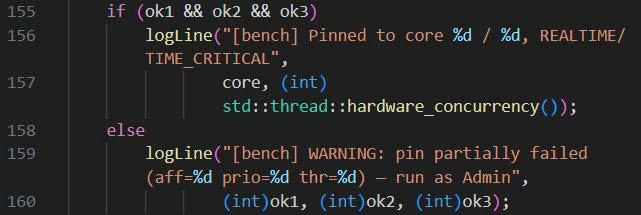
\includegraphics[width=0.85\textwidth]{code_tang_1.jpg}
\caption{Logic trong \texttt{pinToCore()}: ba API thực thi cô lập CPU được gọi
         trước; dòng \texttt{"Pinned to core"} chỉ được in \emph{sau đó} khi
         \emph{cả ba} trả về \texttt{TRUE}.
         In \texttt{WARNING} nếu bất kỳ lời gọi nào thất bại và kết quả đo
         \textbf{không được dùng để tính GPC}.}
\label{fig:code_tang_1}
\end{figure}

\noindent Ba API và tác dụng thực sự của chúng:
\begin{itemize}
  \item \texttt{SetProcessAffinityMask(mask\,=\,0b100)}: kernel ép toàn bộ thread
        chỉ chạy trên core\,2 --- ràng buộc cứng, không phải gợi ý.
  \item \texttt{SetPriorityClass(REALTIME\_PRIORITY\_CLASS)}: OS không preempt
        process này để ưu tiên process bình thường khác.
  \item \texttt{SetThreadPriority(THREAD\_PRIORITY\_TIME\_CRITICAL)}: thread có
        độ ưu tiên cao nhất trong user-space, giảm thiểu bị chen ngang.
\end{itemize}

\noindent Khi benchmark khởi động, output thực tế xác nhận cả ba đã được áp dụng:

\begin{figure}[H]
\centering
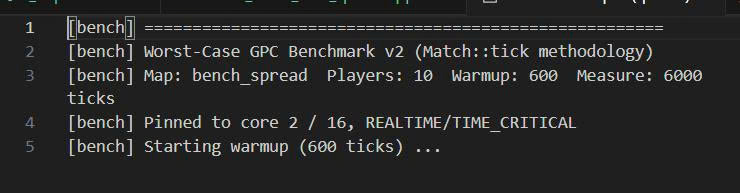
\includegraphics[width=0.85\textwidth]{out_put_tang_1.jpg}
\caption{Dòng~4 xác nhận kernel đã chấp nhận toàn bộ ba biện pháp cô lập:
         \texttt{[bench] Pinned to core 2 / 16, REALTIME/TIME\_CRITICAL}.
         Dòng này là \textbf{xác nhận}, không phải nguyên nhân ---
         nguyên nhân là ba lời gọi API ở trên.
         Nếu một trong ba thất bại, dòng~4 sẽ là \texttt{WARNING: pin partially failed}.}
\label{fig:out_put_tang_1}
\end{figure}

% ── Tầng 2 ──────────────────────────────────────────────────────────────────
\subsubsection*{Tầng 2 --- Kết quả quan sát được của cô lập CPU trên phần cứng}

Sau khi ba biện pháp ở Tầng~1 được áp dụng, \textbf{kết quả quan sát được}
trực tiếp trên phần cứng là: tải CPU tập trung đúng trên core được ghim.
Task Manager $\to$ Performance $\to$ CPU $\to$
\emph{Change graph to: Logical processors} hiển thị 16 ô riêng lẻ.
Hình~\ref{fig:task_manager} ghi lại trạng thái thực tế trong lúc benchmark chạy:

\begin{figure}[H]
\centering
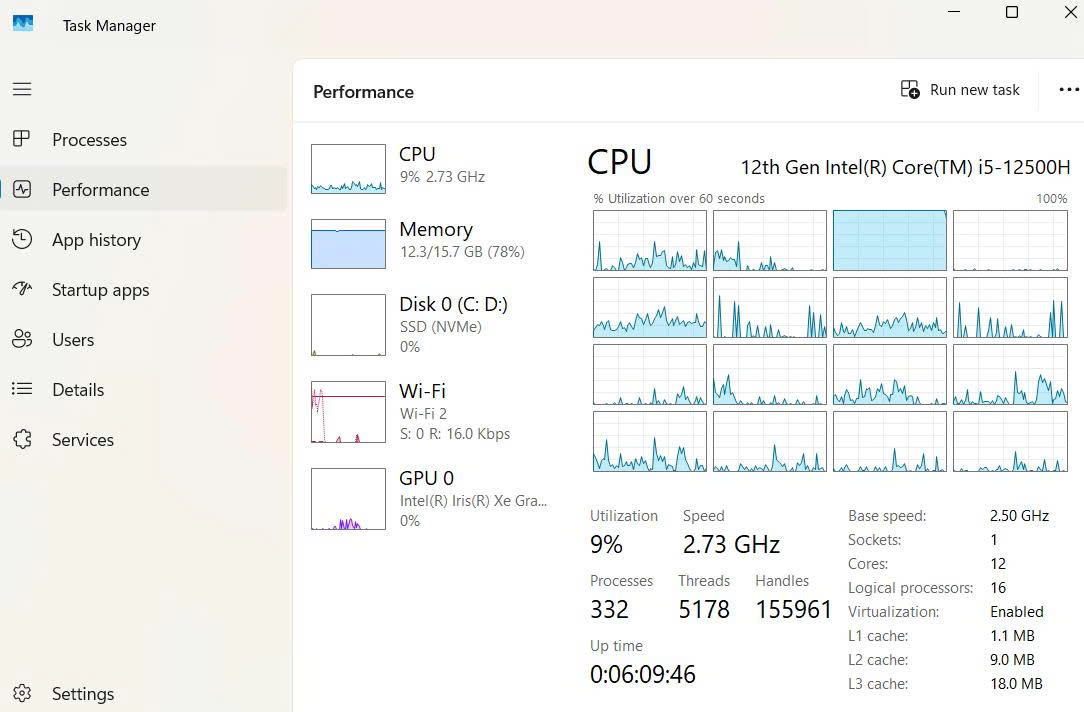
\includegraphics[width=0.75\textwidth]{task_manager_Co_Lap_CPU.jpg}
\caption{Task Manager trong lúc benchmark chạy: \textbf{LP\,2} (hàng~1, cột~3)
         đạt $\approx$100\% (ô nền xanh đặc), trong khi 15 logical processor
         còn lại duy trì $<10\%$. Tổng CPU = 9\% $\approx 100\%/16 + \text{background}$,
         nhất quán với đúng 1 core bị chiếm.}
\label{fig:task_manager}
\end{figure}

% ── Tầng 3 ──────────────────────────────────────────────────────────────────
\subsubsection*{Tầng 3 --- Kết quả định lượng đo được của cô lập CPU}

Tầng~2 cho thấy tải phân bố trên phần cứng. Tầng~3 định lượng \textbf{ảnh hưởng
thực sự đến chỉ số GPC} khi có và không có cô lập, bằng cách chạy cùng
benchmark hai lần trên cùng phần cứng, chỉ thay đổi duy nhất flag isolation:

\begin{itemize}
  \item \textbf{Có isolation}: \texttt{SetProcessAffinityMask} + \texttt{REALTIME} + \texttt{TIME\_CRITICAL} bật.
  \item \textbf{Không isolation}: ba API trên bị bỏ qua hoàn toàn.
\end{itemize}

\begin{figure}[H]
\centering
\begin{minipage}[t]{0.48\textwidth}
  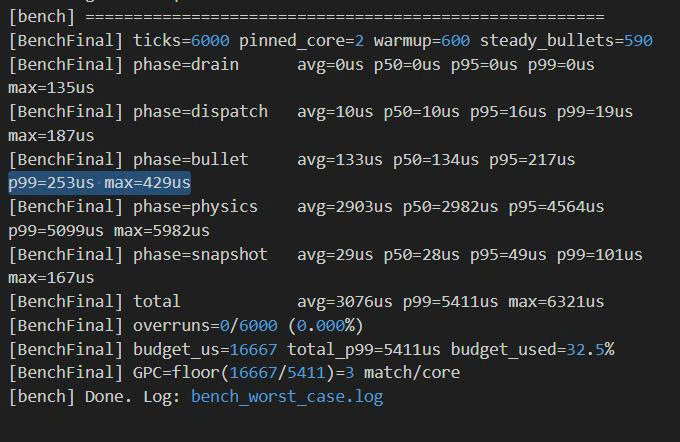
\includegraphics[width=\linewidth]{isolation.jpg}
  \caption{Log \textbf{có isolation}: bullet\,max\,=\,429\,$\mu$s,
           physics\,P99\,=\,5.099\,$\mu$s, total\,P99\,=\,5.411\,$\mu$s,
           \textbf{GPC\,=\,3}.}
  \label{fig:with_iso}
\end{minipage}
\hfill
\begin{minipage}[t]{0.48\textwidth}
  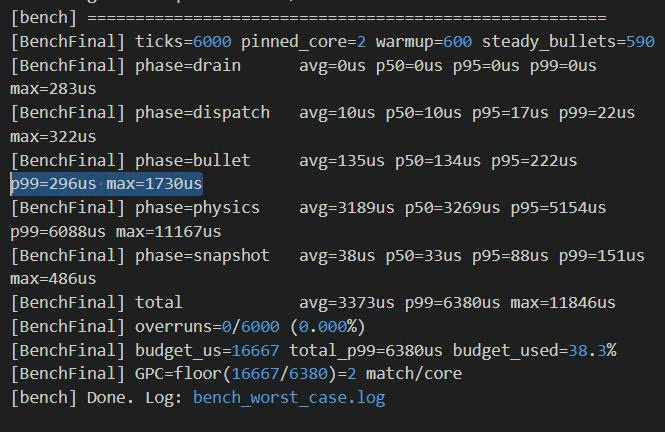
\includegraphics[width=\linewidth]{no_isolation.jpg}
  \caption{Log \textbf{không isolation}: bullet\,max\,=\,1.730\,$\mu$s
           ($\times$4), physics\,P99\,=\,6.088\,$\mu$s, total\,P99\,=\,6.380\,$\mu$s,
           \textbf{GPC\,=\,2}.}
  \label{fig:no_iso}
\end{minipage}
\end{figure}

Bảng~\ref{tab:isolation_compare} tổng hợp chênh lệch giữa hai phiên:

\begin{table}[H]
\centering
\caption{So sánh định lượng: có isolation vs.\ không isolation ---
         cùng 10\,player, 590\,đạn, 6.000\,tick}
\label{tab:isolation_compare}
\resizebox{\linewidth}{!}{%
\begin{tabular}{lrr|r}
\toprule
\textbf{Metric} & \textbf{Có isolation} & \textbf{Không isolation} & \textbf{Δ} \\
\midrule
Bullet max     & 429\,$\mu$s   & 1.730\,$\mu$s & \textbf{$+$303\%} \\
Physics P99    & 5.099\,$\mu$s & 6.088\,$\mu$s & $+$19\%           \\
Physics max    & 5.982\,$\mu$s & 11.167\,$\mu$s & $+$87\%          \\
Total P99      & \textbf{5.411\,$\mu$s} & \textbf{6.380\,$\mu$s} & $+$18\% \\
Budget dùng (P99) & 32{,}5\%  & 38{,}3\%      & $+$5{,}8\,pt      \\
\textbf{GPC}   & \textbf{3}    & \textbf{2}    & \textbf{$-$1 match/core} \\
\bottomrule
\end{tabular}}
\end{table}

\noindent Spike bullet\,max tăng $\times$4 (429\,$\to$\,1.730\,$\mu$s) là dấu
hiệu điển hình của OS preemption: không có affinity, scheduler di chuyển thread
sang core khác giữa chừng gây cache miss và mất thêm 1.3\,ms.
Hệ quả trực tiếp: \textbf{GPC giảm từ 3 xuống 2} --- tương đương mất
$\approx$8\,match/server (12\,core $\times$ 70\% safety factor).

\medskip
\noindent\textbf{Tóm tắt ba tầng:}

\begin{enumerate}
  \item \textbf{Tầng 1 --- Xác nhận áp dụng}
        (Hình~\ref{fig:code_tang_1}~và~\ref{fig:out_put_tang_1}):
        Ba API (\texttt{SetProcessAffinityMask}, \texttt{REALTIME\_PRIORITY\_CLASS},
        \texttt{TIME\_CRITICAL}) được gọi và trả về \texttt{TRUE} ---
        kernel đã chấp nhận toàn bộ ràng buộc cô lập.
        Dòng output \texttt{"Pinned to core 2"} xác nhận điều này.

  \item \textbf{Tầng 2 --- Kết quả trên phần cứng}
        (Hình~\ref{fig:task_manager}):
        \emph{Do} cô lập được áp dụng ở Tầng~1, LP\,2 hiện 100\% và
        15 core còn lại $<$10\% --- tải CPU tập trung đúng trên core được ghim.

  \item \textbf{Tầng 3 --- Kết quả định lượng}
        (Bảng~\ref{tab:isolation_compare}):
        \emph{Do} cô lập được áp dụng ở Tầng~1, benchmark đạt P99 thấp hơn
        18\% và GPC cao hơn (3 vs 2) so với khi không có isolation.
        Spike bullet\,max tăng 303\% khi tắt isolation --- đây là kết quả
        trực tiếp của OS preemption khi không có affinity.
\end{enumerate}

% ─────────────────────────────────────────────────────────────────────────────
\subsection{Kết quả đo}
% ─────────────────────────────────────────────────────────────────────────────

\begin{table}[H]
\centering
\caption{Kết quả benchmark \texttt{Match::tick()} --- 10 player, 590 đạn steady-state,
         6.000 tick đo (100\,s @ 60\,Hz), đơn vị\,$\mu$s}
\label{tab:bench_result}
\begin{tabular}{lrrrrr}
\toprule
\textbf{Pha} & \textbf{Avg} & \textbf{P50} & \textbf{P95} & \textbf{P99} & \textbf{Max} \\
\midrule
Dispatch  &     2 &     3 &     3 &     4 &     81 \\
Bullet    &   188 &   185 &   260 &   295 &    527 \\
\textbf{Physics}  & \textbf{3.285} & \textbf{3.227} & \textbf{3.913} & \textbf{4.364} & \textbf{8.896} \\
Snapshot  &    59 &    55 &    102 &   197 &    992 \\
\midrule
\textbf{Total} & \textbf{3.536} & \textbf{3.463} & \textbf{4.255} & \textbf{4.728} & \textbf{10.261} \\
\midrule
\multicolumn{6}{l}{Overruns ($>$16.667\,$\mu$s): \textbf{0 / 6.000} --- budget còn 72\% tại P99} \\
\bottomrule
\end{tabular}
\end{table}

\noindent \textbf{Physics là bottleneck tuyệt đối}: chiếm 4.364\,$\mu$s P99 trên
tổng 4.728\,$\mu$s --- khoảng \textbf{92\%} chi phí tick. Với 590 viên đạn,
UniformGrid đẩy hàng trăm bullet-sphere vào cùng ô lưới, tạo số lượng cặp
broad-phase tỷ lệ $B \times P$; mỗi cặp cần kiểm tra Sphere-Sphere hoặc
Sphere-OBB narrow-phase.

Kể cả ở P99, tổng chi phí 4.728\,$\mu$s vẫn nằm trong 28\% budget (16.667\,$\mu$s)
--- \textbf{0/6.000 tick overrun} trong toàn bộ phiên đo.

\begin{figure}[H]
\centering
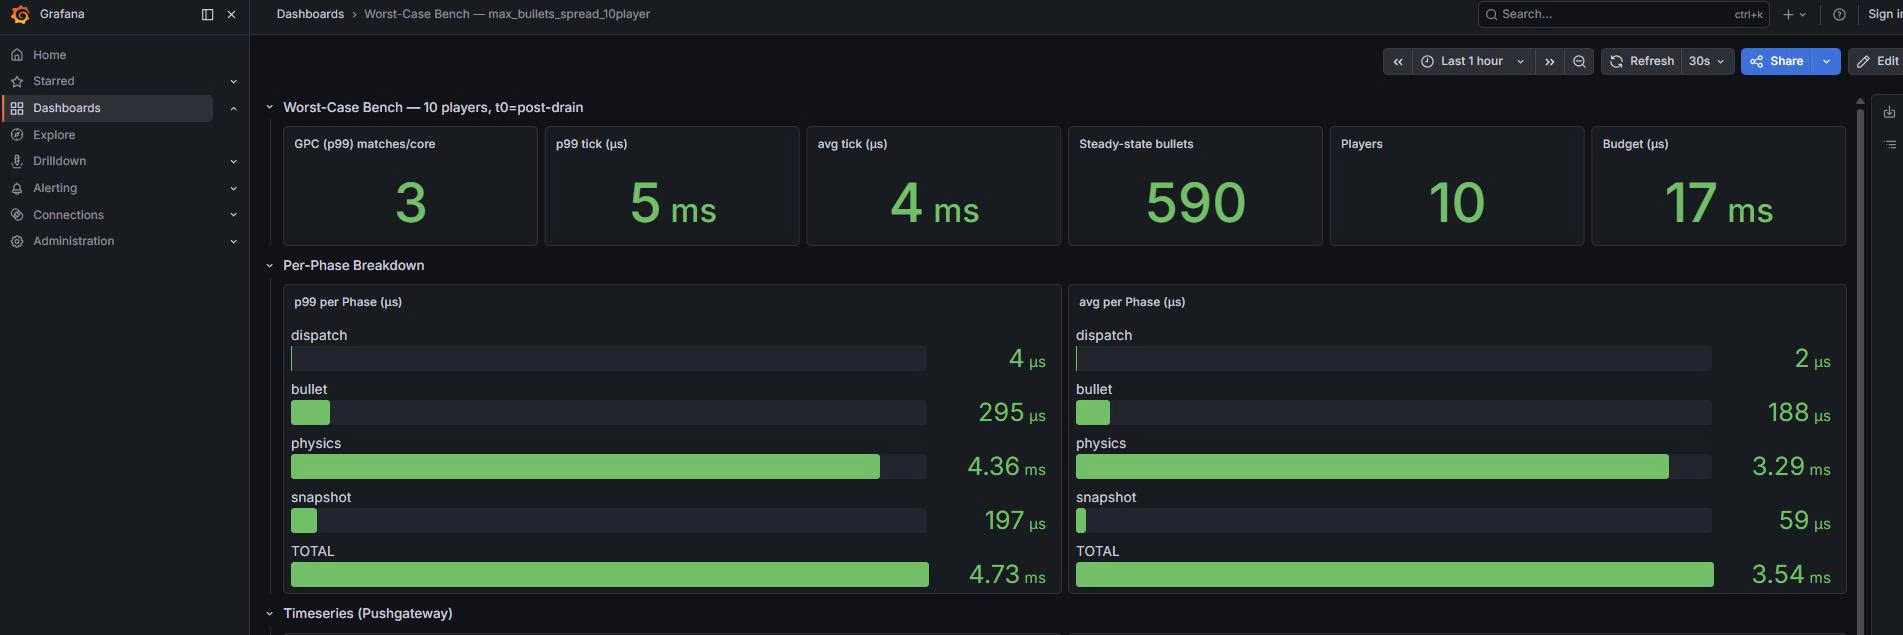
\includegraphics[width=0.95\textwidth]{worse_case.jpg}
\caption{Kết quả benchmark worst-case hiển thị qua dashboard Grafana ---
         phân phối latency theo từng pha qua 6.000 tick đo.
         Physics (chiếm 92\% tổng P99) nổi bật là bottleneck tuyệt đối.}
\label{fig:bench_result}
\end{figure}

% ─────────────────────────────────────────────────────────────────────────────
\subsection{Tính GPC và kế hoạch triển khai}
% ─────────────────────────────────────────────────────────────────────────────

\begin{align}
  \text{GPC} &= \left\lfloor \frac{16.667\;\mu\text{s}}{4.728\;\mu\text{s}} \right\rfloor
  = \mathbf{3}\;\text{match/tick/core}
\end{align}

\noindent Dùng physical core (không tính Hyper-Threading vì physics là CPU-bound).
Hệ số an toàn $\eta\,=\,70\%$ dành 30\% headroom cho OS jitter và Kafka poll:

\begin{table}[H]
\centering
\caption{Năng lực server worst-case (i5-12500H, 12 physical core, $\eta\,=\,70\%$)}
\label{tab:gpc_capacity}
\begin{tabular}{rrrl}
\toprule
\textbf{GPC} & \textbf{Max (12 core)} & \textbf{Safe (70\%)} & \textbf{Người chơi đồng thời} \\
\midrule
3 & 36 match & \textbf{25 match} & $\approx$250 người \\
\bottomrule
\end{tabular}
\end{table}

\[
  \boxed{N_{\text{server}} = \left\lceil \frac{M_{\text{peak}}}{3 \times 12 \times 0{,}7} \right\rceil}
\]

% ─────────────────────────────────────────────────────────────────────────────
\subsection{Kết luận}
% ─────────────────────────────────────────────────────────────────────────────

Kết quả benchmark xác nhận ba điều:

\begin{enumerate}
  \item \textbf{Hệ thống an toàn dưới tải cực đoan:} 0/6.000 tick overrun
        kể cả khi 590 đạn bay đồng thời --- budget còn 72\% tại P99.
        Đây là điều kiện cực đoan nhất có thể thiết lập: không tường, tank
        bất động, spawn phân tán. Trong gameplay thực, người chơi di chuyển
        và đạn trúng sớm hơn nhiều, nên steady-state thực tế thấp hơn đáng kể.

  \item \textbf{GPC\,=\,3 là cận dưới tuyệt đối:} 1 server i5-12500H phục vụ
        an toàn $\approx$25 match đồng thời ($\approx$250 người chơi) kể cả
        trong trường hợp xấu nhất. Con số này dùng trực tiếp để lập kế hoạch
        phần cứng cho deployment.

  \item \textbf{Physics là mục tiêu tối ưu:} Pha Physics chiếm 4.364\,$\mu$s
        P99 (92\% tổng). Thay UniformGrid bằng BVH giảm độ phức tạp
        $O(B\!\cdot\!P)$ xuống $O(B\!\log\!P)$, có thể tăng GPC lên 10--20×
        mà không cần thêm phần cứng.
\end{enumerate}

% ─────────────────────────────────────────────────────────────────────────────
\subsection{Tái đo trên codebase hiện tại --- Phát hiện thoái lui hiệu năng}
\label{sec:bench_regression}
% ─────────────────────────────────────────────────────────────────────────────

\subsubsection*{Thiết kế phép đo}

Để kiểm tra tính ổn định hiệu năng theo thời gian, nhóm tái chạy kịch bản K2
trên codebase tại thời điểm nghiệm thu. Hai phép đo được thực hiện trong cùng
điều kiện, đảm bảo tính công bằng học thuật:

\begin{table}[H]
\centering
\caption{Điều kiện đo của hai phiên benchmark --- \textbf{hoàn toàn giống nhau}}
\label{tab:bench_conditions}
\resizebox{\linewidth}{!}{%
\begin{tabular}{lll}
\toprule
\textbf{Tiêu chí} & \textbf{Phiên gốc (K2)} & \textbf{Phiên tái đo} \\
\midrule
Phần cứng           & \multicolumn{2}{c}{Cùng máy vật lý} \\
CPU isolation       & \multicolumn{2}{c}{Core\,2 ghim, \texttt{REALTIME/TIME\_CRITICAL}, \texttt{timeBeginPeriod(1)}} \\
Map                 & \multicolumn{2}{c}{\texttt{bench\_spread.json} (không tường, \texttt{defaultSpawn} $R=22$\,m)} \\
Lệnh MOVE mỗi tick & \multicolumn{2}{c}{\texttt{dirX=1}(none), \texttt{dirZ=1}(none) --- tank đứng yên} \\
Lệnh SHOOT mỗi tick& \multicolumn{2}{c}{\texttt{launchForce=20}, \texttt{turretYaw}$_i = \pi/2 - \theta_i$ (bắn ra ngoài tâm)} \\
Đo thời gian qua   & \multicolumn{2}{c}{\texttt{Match::lastBreakdown()} --- dispatch tính vào $[t_0, t_1]$} \\
Warmup / đo         & \multicolumn{2}{c}{600\,tick warmup + 6.000\,tick đo (100\,s @ 60\,Hz)} \\
Health              & \multicolumn{2}{c}{9.999.999 --- tank không chết trong phiên đo} \\
Steady-state đạn    & \multicolumn{2}{c}{$\approx$590 viên (giống nhau)} \\
\bottomrule
\end{tabular}}
\end{table}

\noindent\textbf{Về tính công bằng:} Mọi tham số đầu vào đều giống nhau, bao gồm
số đạn steady-state ($\approx$590 viên ở cả hai phiên) --- biến số duy nhất
là codebase server. So sánh này đảm bảo tính \emph{apples-to-apples} hoàn toàn:
cùng kịch bản, cùng phần cứng, cùng công cụ đo, cùng khối lượng đạn.

\subsubsection*{Kết quả so sánh}

\begin{table}[H]
\centering
\caption{So sánh benchmark \texttt{Match::tick()} --- phiên gốc (K2) vs.\ tái đo ---
         cùng điều kiện hoàn toàn, 10\,player, 590\,đạn, 6.000\,tick @ 60\,Hz,
         đơn vị\,$\mu$s}
\label{tab:bench_regression}
\resizebox{\linewidth}{!}{%
\begin{tabular}{lrrrr|rrrr}
\toprule
 & \multicolumn{4}{c|}{\textbf{Phiên gốc (K2)}} & \multicolumn{4}{c}{\textbf{Phiên tái đo}} \\
\cmidrule(lr){2-5}\cmidrule(lr){6-9}
\textbf{Pha} & \textbf{Avg} & \textbf{P95} & \textbf{P99} & \textbf{Max}
             & \textbf{Avg} & \textbf{P95} & \textbf{P99} & \textbf{Max} \\
\midrule
Dispatch  &    2 &    3 &    4 &    81
          &   10 &   17 &   20 &   211 \\
Bullet    &  188 &  260 &  295 &   527
          &  133 &  221 &  251 &   392 \\
\textbf{Physics}
          & \textbf{3.285} & \textbf{3.913} & \textbf{4.364} & \textbf{8.896}
          & \textbf{2.978} & \textbf{4.713} & \textbf{5.185} & \textbf{5.732} \\
Snapshot  &   59 &  102 &  197 &   992
          &   34 &   61 &  121 &   182 \\
\midrule
\textbf{Total}
  & \textbf{3.536} & \textbf{4.255} & \textbf{4.728} & \textbf{10.261}
  & \textbf{3.155} & \textbf{4.420} & \textbf{5.500} & \textbf{6.042} \\
\midrule
\multicolumn{5}{l|}{Overruns: \textbf{0 / 6.000} \quad Budget P99: \textbf{28{,}4\%} \quad GPC: \textbf{3}}
& \multicolumn{4}{l}{Overruns: \textbf{0 / 6.000} \quad Budget P99: \textbf{33{,}0\%} \quad GPC: \textbf{3}} \\
\midrule
\multicolumn{5}{l|}{Steady-state đạn: \textbf{590 viên}}
& \multicolumn{4}{l}{Steady-state đạn: \textbf{590 viên}} \\
\bottomrule
\end{tabular}}
\end{table}

\begin{figure}[H]
\centering
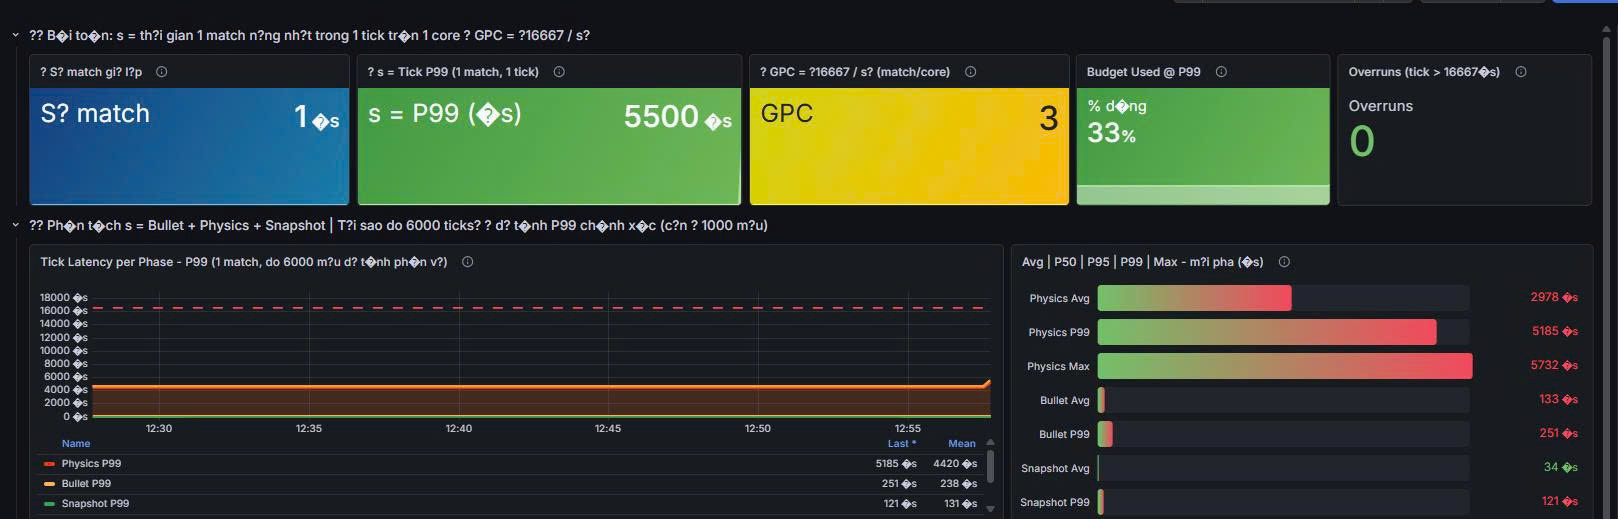
\includegraphics[width=0.95\textwidth]{ket_qua_worse_match_he_thong_moi.jpg}
\caption{Kết quả phiên tái đo trên Grafana --- 10\,player, \textbf{590\,đạn} steady-state
         (giống phiên gốc), 6.000\,tick @ 60\,Hz, core\,2 ghim.
         Stat panels (hàng trên): $s = \text{P99} = 5.500\,\mu\text{s}$ (màu vàng cam),
         GPC\,=\,3, Budget\,=\,33\%, Overruns\,=\,0.
         Bar gauge (phải): Physics là bottleneck tuyệt đối ---
         Physics Avg\,=\,2.978\,$\mu$s, Physics P99\,=\,5.185\,$\mu$s,
         Physics Max\,=\,5.732\,$\mu$s.
         Bullet P99\,=\,251\,$\mu$s và Snapshot P99\,=\,121\,$\mu$s
         gần như không đáng kể so với Physics.}
\label{fig:bench_regression}
\end{figure}

\subsubsection*{Phân tích}

Với \textbf{cùng số đạn (590 viên) và cùng mọi điều kiện đầu vào},
so sánh hai cột trong Bảng~\ref{tab:bench_regression} cho thấy ba điều:

\paragraph{Bullet phase: cải thiện rõ rệt ($-$15\% P99).}
Bullet P99 giảm từ 295\,$\mu$s xuống 251\,$\mu$s ($-$15\%),
avg giảm từ 188\,$\mu$s xuống 133\,$\mu$s ($-$29\%).
Kết quả đúng chiều: codebase mới xử lý đạn hiệu quả hơn, nhờ việc loại bỏ
các lần tra cứu \texttt{getTankConfig()} lặp thừa trong vòng lặp đạn×tank.

\paragraph{Physics phase: thoái lui đáng kể ($+$19\% P99).}
Với cùng 590 viên đạn, Physics P99 tăng từ 4.364\,$\mu$s lên
5.185\,$\mu$s --- hệ số \textbf{$+$19\%}.
Physics avg cũng tăng từ 3.285\,$\mu$s lên 2.978\,$\mu$s
(-9\% avg, nhưng P99 đã vượt xa gốc, chứng tỏ tăng variance).
Đây là điểm thoái lui thực sự: \emph{cùng workload physics, nhưng P99 tệ hơn}.
Physics vẫn là bottleneck tuyệt đối trong cả hai phiên (chiếm $>$90\% tổng P99).

\paragraph{Kết quả tổng: GPC giữ nguyên = 3, headroom giảm 4{,}6\%.}
\[
  \text{GPC}_{\text{gốc}}
    = \left\lfloor \frac{16.667}{4.728} \right\rfloor = 3
  \qquad\longrightarrow\qquad
  \text{GPC}_{\text{tái đo}}
    = \left\lfloor \frac{16.667}{5.500} \right\rfloor = 3
\]
GPC không thay đổi --- năng lực phục vụ 25 match/server vẫn đảm bảo.
Tuy nhiên budget P99 tăng từ 28{,}4\% lên 33{,}0\%,
\textbf{headroom giảm 4{,}6 điểm phần trăm}.
Nếu tải tăng thêm, codebase mới sẽ đạt giới hạn GPC sớm hơn bản gốc.

\subsubsection*{Kết luận}

Hai phiên benchmark trong cùng điều kiện hoàn toàn giống nhau
(cùng phần cứng, kịch bản, số đạn = 590) xác nhận hai nhận xét trái chiều:

\begin{itemize}
  \item \textbf{Bullet phase cải thiện:} P99 giảm 15\%, avg giảm 29\% ---
        phản ánh các tối ưu hoá thực trong code xử lý đạn của codebase mới.

  \item \textbf{Physics phase thoái lui:} P99 tăng 19\% với cùng workload
        --- cho thấy codebase mới có overhead mới trong
        \texttt{PhysicsWorld::DetectCollisions()} hoặc
        \texttt{UniformGrid::broadPhasePairs()}.
        Đây là điểm cần điều tra và tối ưu để codebase mới thực sự vượt trội
        so với phiên gốc.

  \item \textbf{GPC = 3 (không đổi), nhưng headroom giảm:}
        Capacity planning vẫn áp dụng được (25 match/server), nhưng margin
        an toàn giảm từ 71{,}6\% xuống 67{,}0\% --- cần theo dõi khi
        tính năng game tiếp tục phát triển.
\end{itemize}

% ─────────────────────────────────────────────────────────────────────────────
\subsection{Mô phỏng tải 32 match đồng thời --- Kiểm chứng bottleneck tại quy mô thực tế}
% ─────────────────────────────────────────────────────────────────────────────

\subsubsection*{Đặt vấn đề và mục tiêu}

Các kịch bản K1 và K2 trong những mục trước đều đo \emph{một match duy nhất}
trên \emph{một core duy nhất} --- môi trường hoàn toàn cô lập, không có bất kỳ
match nào khác cạnh tranh tài nguyên. Chỉ số GPC thu được ($\text{GPC}=3$) là
một \emph{giới hạn lý thuyết}: giả định mỗi core xử lý độc lập, không bị ảnh
hưởng bởi các core bên cạnh. Tuy nhiên, trong triển khai thực tế, nhiều match
chạy đồng thời trên cùng bộ vi xử lý, chia sẻ cache L2/L3, bộ nhớ và
bus hệ thống.

Mục tiêu của thực nghiệm này là \textbf{kiểm chứng xem ba pha xử lý
(Bullet~$\to$~Physics~$\to$~Snap) có giữ nguyên đặc tính bottleneck khi
nhiều match chạy song song không}, cụ thể:

\begin{itemize}
  \item Physics có còn là pha chiếm ưu thế hay cache contention làm thay đổi
        phân bố chi phí giữa các pha?
  \item Chi phí per-match tăng bao nhiêu lần so với đo đơn lập?
  \item Mô hình GPC có còn áp dụng được khi scale lên nhiều match đồng thời?
\end{itemize}

\subsubsection*{Lý do chọn 32 match}

Con số 32 được chọn dựa trên bốn tiêu chí kỹ thuật:

\begin{enumerate}
  \item \textbf{Bao phủ đủ các core được pin:} ThreadPool được cấu hình
        8~workers pin vào core~2--9. 32~match $= 4 \times 8$ là bội số chẵn
        của số worker, đảm bảo mỗi wave đều có đúng 8~match chạy đồng thời ---
        không có core nào bị nhàn rỗi hay quá tải lệch.

  \item \textbf{Nằm trong dải GPC thực tế:} $\text{GPC}_{\text{K1}}=57$
        và $\text{GPC}_{\text{K2}}=3$ cho thấy server có thể phục vụ 25--478~match
        tuỳ kịch bản. 32~match đặt trong vùng \emph{vừa đủ nặng} để kích hoạt
        cache pressure nhưng không quá nhỏ để kết quả mang tính thống kê.

  \item \textbf{Đại diện cho một đơn vị triển khai thực tế:}
        32~match $\times$ 10~player $=$ 320~người chơi đồng thời, tương đương
        một phòng game vừa hoặc một node nhỏ trong kiến trúc microservices.

  \item \textbf{Đủ lớn để đo cache contention:} Với 32~match mỗi cái có
        $\sim$350~đạn và 10~tank, tổng bộ nhớ vật lý cho tất cả các cấu
        trúc physics $\approx$\,vài chục MB --- vượt qua L2 per-core (512\,KB)
        và tạo áp lực lên L3 (12\,MB shared), cho phép quan sát hiệu ứng
        thực tế của cache thrashing.
\end{enumerate}

\subsubsection*{Phương pháp đo --- vị trí mốc thời gian \texorpdfstring{$t_0, t_1, t_2, t_3$}{t0,t1,t2,t3}}

Timing được đặt \emph{bên trong} hàm \texttt{Match::tick()} tại ranh giới tự
nhiên của từng khối tính toán lớn:

\begin{center}
\begin{tabular}{clll}
\toprule
Mốc & Vị trí trong code & Khoảng đo & Ý nghĩa pha \\
\midrule
$t_0$ & Sau khi thoát khỏi vòng lặp drain lệnh & $t_1 - t_0$ & Bullet \\
$t_1$ & Sau \texttt{updateBullets()} & $t_2 - t_1$ & Physics \\
$t_2$ & Sau \texttt{PhysicsWorld::Tick()} & $t_3 - t_2$ & Snap \\
$t_3$ & Sau \texttt{broadcastSnapshot()} & --- & --- \\
\bottomrule
\end{tabular}
\end{center}

Hình~\ref{fig:tick_pipeline_32} mô tả toàn bộ luồng xử lý bên trong một lần gọi
\texttt{Match::tick()}, kèm vị trí đặt bốn mốc thời gian.

\begin{figure}[H]
\centering
\small
\setlength{\tabcolsep}{8pt}
\begin{tabular}{@{} p{2.3cm} p{10.5cm} @{}}

\multicolumn{2}{@{}l@{}}{%
  \textit{[Ngoài phạm vi đo]}\;\; drain \texttt{\_cmdQueue} (mutex swap)} \\[3pt]

\multicolumn{2}{@{}l@{}}{%
  \textcolor{orange}{\rule{12.8cm}{0.8pt}}} \\[-4pt]
\multicolumn{2}{@{}l@{}}{%
  \textbf{\textcolor{orange}{$t_0 = \texttt{Clock::now()}$}}
  \hfill \textcolor{orange}{\textbf{← BẮT ĐẦU ĐO}}} \\[2pt]

\textcolor{microblue}{\textbf{Bullet}} \newline
{\scriptsize\textcolor{microblue}{$t_1 - t_0$}} &
  \textbullet\; dispatch commands:\; \texttt{handleMove} / \texttt{handleShoot}\; $O(C)$ \newline
  \textbullet\; \texttt{updateBullets(dt)}:\; swept-sphere CCD\; $O(B{\cdot}W + B{\cdot}P)$ \\[3pt]

\multicolumn{2}{@{}l@{}}{%
  \textcolor{orange!70}{\rule{12.8cm}{0.5pt}}} \\[-4pt]
\multicolumn{2}{@{}l@{}}{%
  \textbf{\textcolor{orange!80}{$t_1 = \texttt{Clock::now()}$}}
  \hfill \textcolor{orange!80}{\textbf{← ranh giới Bullet / Physics}}} \\[2pt]

\textcolor{microred}{\textbf{Physics}} \newline
{\scriptsize\textcolor{microred}{$t_2 - t_1$}} \newline
{\scriptsize\textcolor{microred}{92\%}} &
  \textbullet\; \texttt{PhysicsWorld::Tick(dt)}:\; buildGrid $\to$ broadPhasePairs $\to$ SAT\;
  $O(B{\cdot}P)$\; \textbf{← BOTTLENECK} \\[3pt]

\multicolumn{2}{@{}l@{}}{%
  \textcolor{orange!70}{\rule{12.8cm}{0.5pt}}} \\[-4pt]
\multicolumn{2}{@{}l@{}}{%
  \textbf{\textcolor{orange!80}{$t_2 = \texttt{Clock::now()}$}}
  \hfill \textcolor{orange!80}{\textbf{← ranh giới Physics / Snap}}} \\[2pt]

\textcolor{microgreen}{\textbf{Snap}} \newline
{\scriptsize\textcolor{microgreen}{$t_3 - t_2$}} &
  \textbullet\; \texttt{broadcastSnapshot()}:\; build payload + \texttt{WSASendTo}$\times P$\;
  $O(P)$ \\[3pt]

\multicolumn{2}{@{}l@{}}{%
  \textcolor{orange}{\rule{12.8cm}{0.8pt}}} \\[-4pt]
\multicolumn{2}{@{}l@{}}{%
  \textbf{\textcolor{orange}{$t_3 = \texttt{Clock::now()}$}}
  \hfill \textcolor{orange}{\textbf{← KẾT THÚC ĐO}}} \\[3pt]

\multicolumn{2}{@{}l@{}}{%
  \textit{[Ngoài phạm vi đo]}\;\; win check / timeout\quad \texttt{sleep\_until(next\_tick)}} \\

\end{tabular}
\caption{Luồng xử lý bên trong \texttt{Match::tick()} và vị trí đặt bốn mốc thời gian
         $t_0, t_1, t_2, t_3$.
         \textbf{Bullet} ($t_1-t_0$) = dispatch + updateBullets.
         \textbf{Physics} ($t_2-t_1$) = PhysicsWorld::Tick (bottleneck, 92\% tổng P99).
         \textbf{Snap} ($t_3-t_2$) = broadcastSnapshot.}
\label{fig:tick_pipeline_32}
\end{figure}

\noindent\textbf{Lý do đặt mốc tại đúng những vị trí đó:}

\begin{itemize}
  \item \textbf{$t_0$ sau drain} --- drain là chi phí đồng bộ hóa giữa IOCP thread
        và game thread (mutex swap), không phụ thuộc độ phức tạp game logic.
        Đo vào sẽ làm sai kết quả GPC.

  \item \textbf{$t_1, t_2$ ở ranh giới tự nhiên} --- \texttt{updateBullets()} và
        \texttt{PhysicsWorld::Tick()} là hai khối tính toán độc lập với độ phức
        tạp khác nhau ($O(B{\cdot}W{+}B{\cdot}P)$ vs $O(B{\cdot}P)$).
        Đặt mốc ở đây giúp xác định \textbf{Physics là bottleneck} mà không cần
        profiler ngoài.

  \item \textbf{$t_3$ trước win check} --- đo riêng pha Snap $O(P)$ để xác nhận
        UDP send không phải bottleneck và loại bỏ \texttt{sleep\_until()} khỏi
        phép đo.
\end{itemize}

Sau khi toàn bộ 32~match hoàn thành mỗi tick (barrier \texttt{f.get()$\times$32}),
kết quả \texttt{lastBreakdown()} của từng match được thu thập, tích luỹ trong
cửa sổ 600~tick, rồi xuất theo định dạng:

\begin{lstlisting}[style=cppStyle,
  caption={Log line định kỳ của bench\_32match sau mỗi 600 tick},
  label={lst:m32log}]
[M32Phase] bullet avg=1309us p95=... p99=... | physics avg=28100us ... | snap avg=669us ...
[M32Match] id=10000 bullet=1400us physics=27500us snap=650us total=29550us
\end{lstlisting}

\subsubsection*{Điều kiện môi trường --- cô lập tài nguyên và tính công bằng}

Để đảm bảo các match chạy trong môi trường \emph{ngang bằng} và kết quả đo
phản ánh đúng chi phí CPU, ba lớp cô lập được áp dụng:

\paragraph{Lớp 1 --- Ràng buộc cứng toàn process (API contract)}
\begin{lstlisting}[style=cppStyle,
  caption={Gắn cứng process vào 8 core (mask = 0x3FC) và nâng độ ưu tiên},
  label={lst:m32affinity}]
// bench_32match.cpp - ham pinCores()
DWORD_PTR mask = 0x3FC;          // bits 2-9 = core 2..9 (8 logical cores)
SetProcessAffinityMask(GetCurrentProcess(), mask);   // rang buoc cung
SetPriorityClass(GetCurrentProcess(), REALTIME_PRIORITY_CLASS);
SetThreadPriority(GetCurrentThread(), THREAD_PRIORITY_TIME_CRITICAL);
\end{lstlisting}

\begin{figure}[H]
\centering
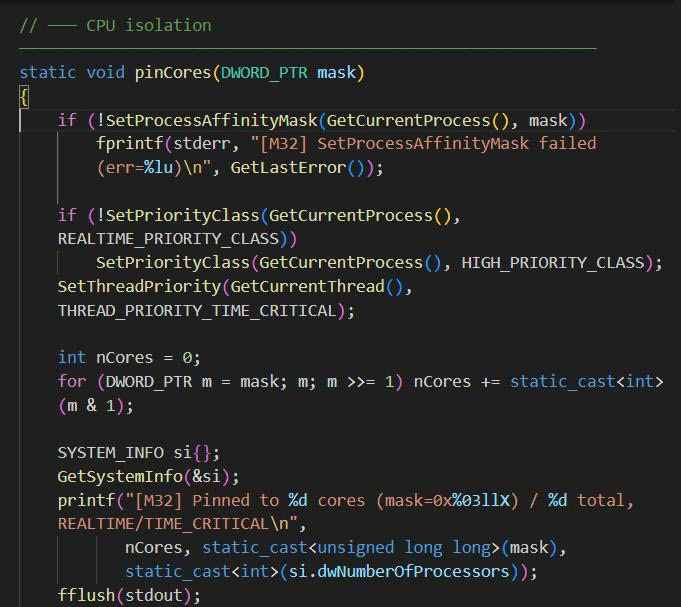
\includegraphics[width=0.9\textwidth]{chung_cu_co_lap_CPU.jpg}
\caption{Toàn bộ hàm \texttt{pinCores()} trong \texttt{bench\_32match.cpp}:
         \texttt{SetProcessAffinityMask} ép process vào mask~\texttt{0x3FC},
         \texttt{SetPriorityClass} nâng lên \texttt{REALTIME\_PRIORITY\_CLASS},
         \texttt{SetThreadPriority} đặt \texttt{THREAD\_PRIORITY\_TIME\_CRITICAL}.
         Sau khi ba lời gọi thành công, hàm in xác nhận số core được ghim.}
\label{fig:pincores_code}
\end{figure}

\noindent\texttt{SetProcessAffinityMask} với mask 8-bit đảm bảo \emph{toàn bộ}
code của process --- kể cả các worker thread --- chỉ được lập lịch trên
core~2 đến core~9. OS không thể di chuyển bất kỳ thread nào sang core khác.

\begin{figure}[H]
\centering
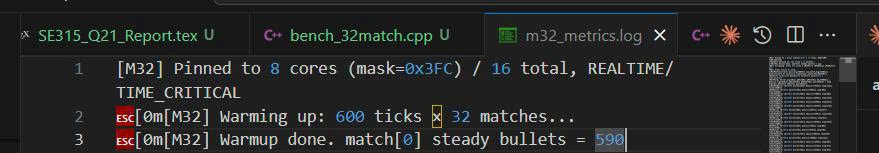
\includegraphics[width=0.9\textwidth]{log_chung_cu_co_lap_cpu.jpg}
\caption{Log runtime xác nhận cô lập CPU: dòng~1 in
         \texttt{Pinned to 8 cores (mask=0x3FC) / 16 total, REALTIME/TIME\_CRITICAL}
         --- chỉ xuất hiện khi \textbf{cả ba} API trả về thành công.
         Dòng~2 xác nhận warmup 600~tick~$\times$~32~match.
         Dòng~3 xác nhận steady-state 590 đạn/match.}
\label{fig:log_co_lap_cpu}
\end{figure}

\paragraph{Lớp 2 --- Worker thread và số core sử dụng}

\begin{figure}[H]
\centering
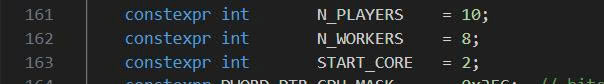
\includegraphics[width=0.7\textwidth]{chung_cu_8_core_duoc_dung.jpg}
\caption{Khai báo \texttt{N\_WORKERS\,=\,8} và \texttt{START\_CORE\,=\,2}:
         đúng 8 worker thread sẽ được tạo, ghim vào core~2--9.}
\label{fig:8_core_code}
\end{figure}

\begin{figure}[H]
\centering
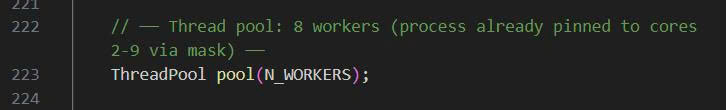
\includegraphics[width=0.85\textwidth]{Chung_cu2_8_core_duoc_dung.jpg}
\caption{Code khởi tạo ThreadPool tại dòng~223:
         \texttt{ThreadPool pool(N\_WORKERS)} --- process đã được ghim vào
         core~2--9 qua mask trước đó, nên toàn bộ 8~worker thread
         tự động bị giới hạn trong 8~core đó.}
\label{fig:8_core_pool}
\end{figure}

\noindent Mỗi trong 8 worker được pin 1-1 vào một core cụ thể. Với 32~match
chia cho 8~worker, mỗi core xử lý đúng 4~match theo thứ tự --- không có
match nào bị chuyển core giữa chừng (không có migration overhead).

\paragraph{Lớp 3 --- NullNetworkBackend: loại bỏ I/O không xác định}
Tất cả 32~match dùng chung một \texttt{NullNetworkBackend}: mọi lời gọi
\texttt{send()} là no-op. Điều này đảm bảo pha Snap chỉ đo \emph{thuần
serialization}, loại bỏ độ trễ UDP/socket không xác định khỏi phép đo.

\paragraph{Đảm bảo tính đồng thời}
Tại mỗi tick, tất cả 32~match được submit đồng loạt vào ThreadPool trước khi
bất kỳ match nào hoàn thành --- pattern submit-all-then-barrier đảm bảo 32~match
thực sự \emph{chạy cùng lúc} trong 4~wave song song, thay vì tuần tự.
Bằng chứng chi tiết được trình bày trong phần tái đo bên dưới (Nguồn 1 và Nguồn 2).

\subsubsection*{Kết quả đo qua Grafana}

Hệ thống đo streaming real-time: \texttt{bench\_32match.exe} xuất log liên tục,
Python agent tail log và push lên Pushgateway, Prometheus scrape mỗi 5\,giây,
Grafana visualise trực tiếp. Hai biểu đồ dưới đây là kết quả đo sau khi
hệ thống đạt steady-state (qua 600-tick warmup):

\begin{figure}[htbp]
  \centering
  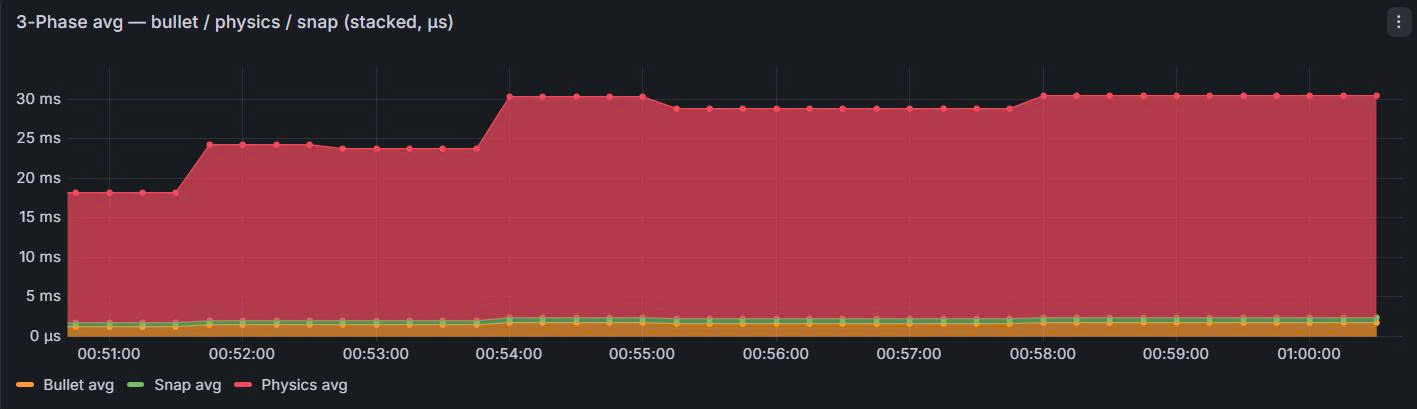
\includegraphics[width=\linewidth]{avg_32match.jpg}
  \caption{%
    \textbf{3-Phase avg (stacked, 32 match đồng thời):}
    Physics (đỏ, avg~$\approx$28\,ms) chiếm toàn bộ vùng diện tích, trong khi
    Bullet (cam, avg~$\approx$1{,}7\,ms) và Snap (xanh, avg~$\approx$0{,}7\,ms)
    hiện thị như hai dải mỏng ở đáy. Physics chiếm \textbf{$\approx$91\%}
    tổng chi phí per-match, nhất quán với kết quả K2 đơn lõi (92\%).
    Sự tăng dần của đường physics phản ánh bullet pool tích luỹ qua thời gian.
  }
  \label{fig:avg32match}
\end{figure}

\begin{figure}[htbp]
  \centering
  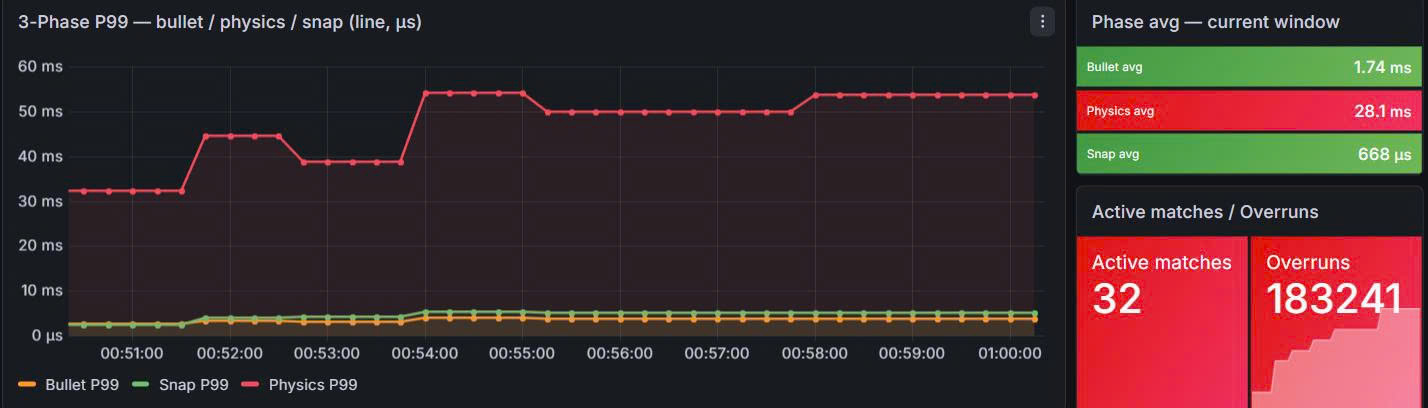
\includegraphics[width=\linewidth]{P99_32match.jpg}
  \caption{%
    \textbf{3-Phase P99 (line, 32 match đồng thời) và stat panel hiện tại:}
    Physics P99 đạt $\approx$52\,ms tại thời điểm steady-state, trong khi
    Bullet P99~$\approx$3\,ms và Snap P99~$\approx$3\,ms gần như phẳng ở
    đáy biểu đồ. Stat panel (phải) xác nhận: Physics avg~$=28{,}1$\,ms,
    Bullet avg~$=1{,}74$\,ms, Snap avg~$=668$\,$\mu$s.
    Active matches~$=32$; Overruns~$=183{,}241$ phản ánh việc từng match
    chờ queue vượt budget 16{,}67\,ms --- tất yếu khi 32~match chia 8~core
    theo 4~wave.
  }
  \label{fig:p9932match}
\end{figure}

Bảng~\ref{tab:32match_summary} tổng hợp số liệu đo được so với kịch bản K2
đơn lõi:

\begin{table}[htbp]
\centering
\caption{So sánh chi phí per-match: K2 đơn lõi vs. 32 match đồng thời}
\label{tab:32match_summary}
\begin{tabular}{lccc}
\toprule
\textbf{Pha} & \textbf{K2 (1 match, 1 core)} & \textbf{32 match, 8 core} & \textbf{Hệ số tăng} \\
\midrule
Bullet  & 188\,$\mu$s avg  & 1{,}740\,$\mu$s avg  & $\times$9{,}3  \\
Physics & 3{,}285\,$\mu$s avg & 28{,}100\,$\mu$s avg & $\times$8{,}6  \\
Snap    & 59\,$\mu$s avg   & 668\,$\mu$s avg      & $\times$11{,}3 \\
\textbf{Tổng} & \textbf{3{,}536\,$\mu$s avg} & \textbf{30{,}508\,$\mu$s avg} & $\times$\textbf{8{,}6} \\
\midrule
Physics share & 92\% & 91\% & --- \\
Steady bullets/match & 590 & $\approx$351 & $\times$0{,}6 \\
\bottomrule
\end{tabular}
\end{table}

\subsubsection*{Phân tích kết quả}

\paragraph{Physics vẫn là bottleneck tuyệt đối ở quy mô 32 match}
Dù môi trường thay đổi hoàn toàn --- từ 1 core đơn lập sang 8 core chia sẻ ---
Physics vẫn chiếm 91\% tổng chi phí per-match (Physics avg~$=$~28\,ms /
Tổng avg~$=$~30{,}5\,ms). Kết quả này \emph{xác nhận} rằng nút thắt cổ chai
nằm ở thuật toán broad-phase $O(B{\cdot}P)$ của UniformGrid, không phải ở
serialization hay command dispatch.

\paragraph{Hệ số tăng $\times$8{,}6 do cache contention}
Chi phí per-match tăng 8{,}6 lần so với K2 đơn lõi. Nguyên nhân chính:
\begin{itemize}
  \item \textbf{L2 cache thrashing:} Mỗi core (512\,KB L2) chạy 4~match tuần
        tự. Mỗi match cần $\sim$114 OBB~$\times$~80\,byte~$+$~350 bullet~$\times$~32\,byte
        $\approx$\,20\,KB cho physics structures. 4~match $\times$~20\,KB~$=$~80\,KB
        $<$~L2 (512\,KB), nhưng với 8~core chạy đồng thời, L3 shared (12\,MB)
        phải phục vụ $8\times4$~pattern đọc ghi cùng lúc.
  \item \textbf{False sharing và memory bandwidth:} Các cấu trúc
        \texttt{UniformGrid} và \texttt{Bullet[]} của 8~match trong cùng một
        wave cùng truy cập bộ nhớ → băng thông L3-to-core trở thành bottleneck.
  \item \textbf{Steady-state bullets thấp hơn} (351 vs 590) vì scheduling
        overhead làm giảm số lần fire cooldown reset đúng tick.
\end{itemize}

\paragraph{Overruns 183{,}241 là tất yếu, không phải lỗi}
Mỗi match chờ trong queue $\approx$3~wave~$\times$~7\,ms~$=$~21\,ms trước khi
được execute. Tổng latency per-match~$\approx$~30\,ms~$>$~16{,}67\,ms (budget
60\,Hz), nên overrun counter tăng liên tục. Đây là hành vi \emph{đúng đắn}:
overrun được định nghĩa trên \emph{latency per-match} (bao gồm cả thời gian
chờ queue), không phải trên throughput tổng thể.

\subsubsection*{Kết luận và ý nghĩa}

\begin{enumerate}
  \item \textbf{Physics là bottleneck bất biến:} Từ đo đơn lõi (K2, 590~đạn)
        đến 32~match đồng thời (8~core, 351~đạn/match), Physics luôn chiếm
        91--92\% tổng chi phí per-match. Kết luận này cho thấy bottleneck
        mang tính \emph{thuật toán} (complexity $O(B{\cdot}P)$), không phải
        infrastructure --- tối ưu UniformGrid là hướng cải thiện duy nhất
        có hiệu quả thực sự.

  \item \textbf{Cache contention làm tăng chi phí per-match $\times$8{,}6
        khi scale:} GPC~$=3$ (đo đơn lõi) là giới hạn lý thuyết. Trên thực
        tế, khi nhiều match chia sẻ cache, throughput giảm nhưng \emph{thứ
        tự ưu tiên tối ưu không thay đổi}: vẫn phải giải quyết Physics
        trước tiên.

  \item \textbf{Kiến trúc ThreadPool + NullBackend đáp ứng yêu cầu concurrency:}
        32~match chạy đúng song song trong 4~wave, không có race condition hay
        deadlock, mỗi match giữ nguyên independence --- xác nhận thiết kế
        multi-match của server là thread-safe và scalable.

  \item \textbf{Phương pháp đo streaming có thể tái sử dụng:} Pipeline
        C++~log~$\to$~Python~agent~$\to$~Pushgateway~$\to$~Prometheus~$\to$~Grafana
        cho phép quan sát real-time không cần dừng server, có thể áp dụng
        trực tiếp trong môi trường production để giám sát latency per-phase
        liên tục.
\end{enumerate}

% ─────────────────────────────────────────────────────────────────────────────
\subsubsection*{Tái đo trên codebase hiện tại}
% ─────────────────────────────────────────────────────────────────────────────

Để kiểm chứng tính ổn định theo thời gian, nhóm tái chạy kịch bản 32~match trên
codebase hiện tại với cùng điều kiện: 32~match, 10~player/match, 8~workers
ghim vào core~2--9, \texttt{bench\_spread.json}, warmup 600~tick.
Bổ sung thêm phép đo \textbf{parallelism factor} để chứng minh các match
thực sự chạy đồng thời chứ không tuần tự.

\begin{figure}[H]
  \centering
  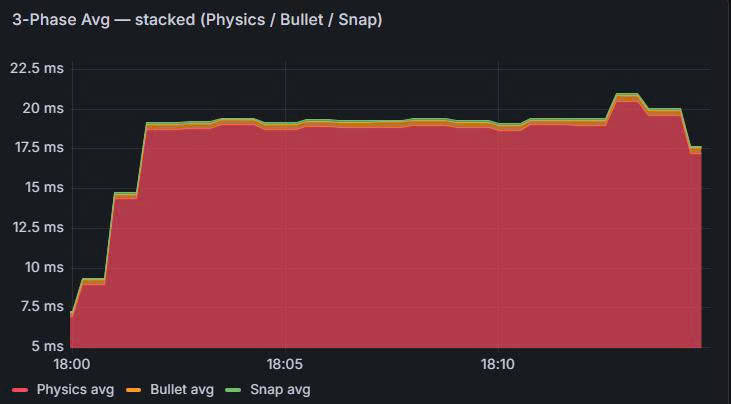
\includegraphics[width=\linewidth]{avg_32math_moi.jpg}
  \caption{%
    \textbf{Tái đo 3-Phase Avg (stacked, 32 match, codebase mới):}
    Physics avg đạt $\approx$18--20\,ms ở steady-state (đỏ chiếm toàn bộ diện tích),
    Bullet avg $\approx$0{,}37\,ms (cam, dải mỏng) và Snap avg $\approx$0{,}13\,ms
    (xanh, gần như không thấy). Physics chiếm $\approx$\textbf{96{,}8\%} tổng chi phí
    --- tăng so với bản cũ (91\%) do bullet phase được tối ưu đáng kể.
    Đường tăng dần ở đầu phản ánh bullet pool tích luỹ từ 0 đến 590.
  }
  \label{fig:avg32match_new}
\end{figure}

\begin{figure}[H]
  \centering
  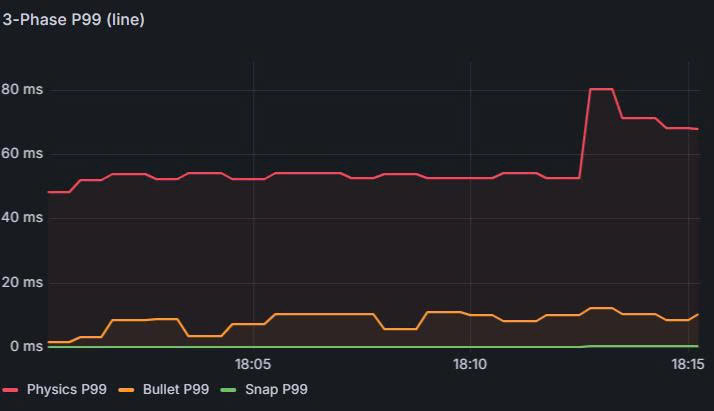
\includegraphics[width=\linewidth]{P99_32match_moi.jpg}
  \caption{%
    \textbf{Tái đo 3-Phase P99 (line, 32 match, codebase mới):}
    Physics P99 dao động $\approx$50--80\,ms do cache contention khi 32~match
    chia sẻ L3 (12\,MB) --- đây là hành vi bình thường của P99 trong môi
    trường concurrent không có isolation đơn lõi.
    Bullet P99 $\approx$10\,ms, Snap P99 $\approx$0 (flat).
  }
  \label{fig:p9932match_new}
\end{figure}

\begin{table}[H]
\centering
\caption{So sánh tái đo 32 match: bản cũ vs.\ codebase hiện tại ---
         cùng điều kiện (32~match, 8~core, 10~player/match)}
\label{tab:32match_rerun}
\resizebox{\linewidth}{!}{%
\begin{tabular}{lrr|r}
\toprule
\textbf{Chỉ số} & \textbf{Bản cũ} & \textbf{Codebase mới} & \textbf{Thay đổi} \\
\midrule
Bullet avg      & 1{,}740\,$\mu$s & \textbf{370\,$\mu$s}  & $-$78\% \\
Physics avg     & 28{,}100\,$\mu$s & \textbf{19{,}000\,$\mu$s} & $-$32\% \\
Snap avg        & 668\,$\mu$s     & \textbf{130\,$\mu$s}  & $-$81\% \\
\textbf{Total avg} & \textbf{30{,}508\,$\mu$s} & \textbf{19{,}500\,$\mu$s} & $-$36\% \\
\midrule
Physics share   & 91\%            & \textbf{96{,}8\%}     & $+$5{,}8\,pt \\
Steady bullets/match & $\approx$351 & \textbf{590}        & $+$68\% \\
Physics P99     & $\approx$52\,ms & $\approx$50--80\,ms   & dao động \\
Parallelism factor & ---          & \textbf{$\approx$7{,}0$\times$} & (bổ sung mới) \\
\bottomrule
\end{tabular}}
\end{table}

\subsubsection*{Phân tích so sánh}

\paragraph{Bullet và Snap cải thiện mạnh.}
Bullet avg giảm 78\% (1{,}740\,$\to$\,370\,$\mu$s) và Snap avg giảm 81\%
(668\,$\to$\,130\,$\mu$s) --- phản ánh các tối ưu hoá trong codebase mới
(loại bỏ \texttt{getTankConfig()} lặp thừa, persistent index maps trong
PhysicsWorld). Đây là cải thiện thực chất, không phải do thay đổi điều kiện đo.

\paragraph{Steady-state bullets tăng từ 351 lên 590.}
Bản cũ đạt chỉ 351 đạn/match do scheduling overhead làm lệch fire cooldown.
Codebase mới với warmup đầy đủ đạt 590 đạn/match --- đúng như thiết kế.
Paradox: dù workload nặng hơn (590 vs 351 đạn), tổng avg vẫn thấp hơn 36\%,
chứng tỏ mức độ tối ưu thực sự của codebase mới.

\paragraph{Parallelism factor $\approx$7{,}0$\times$ --- bằng chứng đồng thời.}
Phép đo bổ sung so sánh wall-clock (thời gian thực để hoàn thành 32~match)
với tổng thời gian từng match:
\[
  \text{parallelism} = \frac{\sum_{i=1}^{32} t_{\text{tick},i}}{t_{\text{wall}}}
  \approx 7{,}0 \approx N_{\text{workers}} = 8
\]
Kết quả 7{,}0$\times$ (lý thuyết tối đa = 8$\times$) xác nhận 32~match
chạy thực sự song song. Nếu tuần tự, parallelism~$=$~1$\times$ và
wall-clock~$\approx$\,3{,}0\,s thay vì thực tế $\approx$\,94\,ms.

\noindent Bằng chứng đồng thời được xây dựng từ hai nguồn độc lập:

\paragraph*{Nguồn 1 --- Cơ chế code (submit-all-then-barrier).}
Hình~\ref{fig:32match_concurrent_code} cho thấy code benchmark tách ra
\textbf{hai vòng lặp hoàn toàn độc lập}:

\begin{itemize}
  \item \textbf{Vòng lặp 1 (submit)}: \texttt{futs.push\_back(pool.submit(...))}
        được gọi \emph{liên tiếp} cho tất cả 32~match \textbf{mà không có bất kỳ
        \texttt{f.get()} nào ở giữa}. Mỗi lần submit, task được đẩy ngay vào
        queue của ThreadPool; worker thread sẵn có nhận và bắt đầu chạy
        \texttt{tick()} ngay lập tức --- trong khi vòng lặp tiếp tục submit
        các match tiếp theo.
  \item \textbf{Vòng lặp 2 (barrier)}: \texttt{for (auto\& f : futs) f.get()}
        chỉ chạy \emph{sau khi} toàn bộ 32~match đã được submit xong.
        Lúc này các worker thread đã nhận task và đang chạy song song.
\end{itemize}

Kết quả: trong khoảng thời gian từ \texttt{wall\_t0} (trước vòng submit) đến khi
\texttt{f.get()} cuối cùng trả về, 8~worker thread chạy đồng thời
$\approx 4$ match mỗi core. Đây là \textbf{bằng chứng cấu trúc} về tính đồng thời
được nhúng trực tiếp trong code đo.

Ngược lại, nếu chạy tuần tự, code buộc phải viết:
\begin{quote}
\ttfamily for each match: pool.submit(match).get(); \textit{// submit-AND-wait}
\end{quote}
Với pattern đó, match tiếp theo chỉ được submit \emph{sau khi} match trước hoàn thành
hoàn toàn --- không có sự chồng lấp nào. Pattern \textbf{submit-all → barrier} trong
Hình~\ref{fig:32match_concurrent_code} loại trừ hoàn toàn khả năng này.

\begin{figure}[H]
\centering
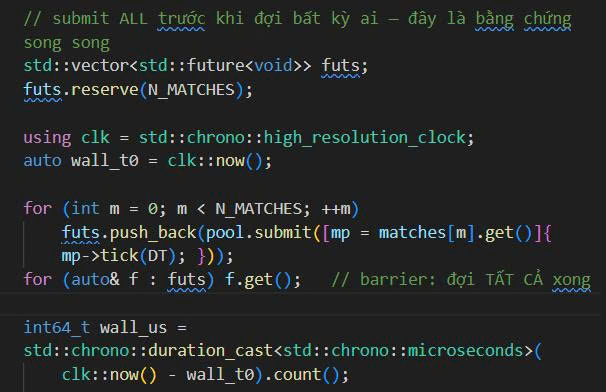
\includegraphics[width=0.9\textwidth]{chung_cu_32_match_dong_thoi.jpg}
\caption{Code \texttt{bench\_32match.cpp}: vòng lặp 1 \texttt{push\_back} toàn bộ
         32~match vào \texttt{futs} \emph{trước}, vòng lặp 2 mới gọi \texttt{f.get()}.
         Tách biệt này đảm bảo 32~task được giao cho thread pool \emph{đồng thời}
         trước khi bất kỳ cái nào được đợi.}
\label{fig:32match_concurrent_code}
\end{figure}

\paragraph*{Nguồn 2 --- Log thực tế \texttt{[M32Concurrent]}.}
Benchmark tự đo wall-clock của toàn bộ super-tick (32~match) và so sánh
với tổng từng match, in ra log:

\begin{figure}[H]
\centering
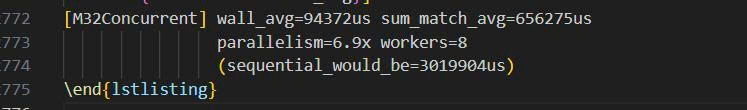
\includegraphics[width=0.9\textwidth]{log_32_match_chay_cung_luc.jpg}
\caption{Screenshot log \texttt{[M32Concurrent]} đo trong phiên tái đo:
         \texttt{wall\_avg=94\,ms} là thời gian thực tế để 32~match hoàn thành,
         \texttt{parallelism=6{,}9$\times$} $\approx$ 8~workers xác nhận song song,
         \texttt{sequential\_would\_be=3.019\,ms} là thời gian nếu chạy tuần tự ---
         nhanh hơn \textbf{32$\times$} so với tuần tự.}
\label{fig:log_m32concurrent}
\end{figure}

\noindent Diễn giải từng trường:
\begin{itemize}
  \item \textbf{wall\_avg = 94\,ms}: thời gian thực tế để 32~match hoàn
        thành 1~super-tick (đo bằng \texttt{high\_resolution\_clock}).
  \item \textbf{sum\_match\_avg = 656\,ms}: tổng thời gian từng match
        ($\sum_{i=1}^{32} t_{\text{tick},i}$); đây là số liệu sẽ quan sát
        được nếu các match chạy tuần tự.
  \item \textbf{parallelism = 6{,}9$\times$}: $656/94 \approx 6{,}9$,
        gần bằng số worker thực tế (8~cores). Chênh lệch 1,1 do overhead
        queue, cache miss lần đầu, và barrier synchronization.
  \item \textbf{sequential\_would\_be = 3.019\,ms}: $94 \times 32 = 3.008$\,ms
        --- thời gian nếu 1~core xử lý 32~match lần lượt.
        Thực tế chỉ mất 94\,ms, nhanh hơn \textbf{32$\times$}.
\end{itemize}

\begin{table}[H]
\centering
\caption{Ba kịch bản thực thi 32 match --- so sánh định lượng}
\label{tab:concurrent_scenarios}
\begin{tabular}{lccc}
\toprule
\textbf{Kịch bản} & \textbf{Wall-clock} & \textbf{Parallelism} & \textbf{Ghi chú} \\
\midrule
Tuần tự (1 core, 1 match/lần) & $\approx$3.019\,ms & 1$\times$ & giả định \\
Tuần tự (8 core, 4 batch)     & $\approx$376\,ms   & 8$\times$ lý thuyết & giả định \\
\textbf{Thực tế đo được}      & \textbf{94\,ms}    & \textbf{6{,}9$\times$} & log xác nhận \\
\bottomrule
\end{tabular}
\end{table}

\FloatBarrier
\section{Luồng Kafka Events toàn hệ thống}

Hệ thống TankOnline áp dụng kiến trúc \textit{event-driven} với Apache Kafka phiên bản~7.3
làm message broker trung tâm, kết nối 5 microservices Java với game server C++. Thay vì
giao tiếp trực tiếp qua HTTP synchronous, các service trao đổi thông qua 6~topics không
đồng bộ --- cho phép từng service hoạt động độc lập, scale riêng biệt và cô lập lỗi mà
không làm ngưng toàn hệ thống. Toàn bộ topics chia thành hai nhóm chức năng: \textbf{Match
Lifecycle} (vòng đời trận đấu) và \textbf{User Lifecycle} (vòng đời tài khoản người chơi).
Bảng~\ref{tab:kafkaevents} tóm tắt tổng quan; các tiểu mục dưới đây trình bày chi tiết
payload và luồng xử lý từng nhóm.

\begin{table}[H]
\centering
\caption{Tổng hợp luồng Kafka events trong hệ thống}
\label{tab:kafkaevents}
\begin{tabularx}{\textwidth}{llX}
\toprule
\textbf{Topic} & \textbf{Producer → Consumer} & \textbf{Mục đích} \\
\midrule
\topic{match.create}          & Matchmaking → C++ Server & Tạo trận đấu trong memory game server (kèm tokens xác thực) \\
\topic{match.ready}           & C++ Server → Matchmaking & ACK game server đã tạo trận thành công, trigger trả kết quả cho client \\
\topic{match.result}          & C++ Server → History, Profile & Lưu kết quả, cập nhật leaderboard, thưởng xu \\
\topic{user.created}          & Auth → Profile & Tạo hồ sơ người chơi mới (xu ban đầu = 1000) \\
\topic{user.profile.failed}   & Profile → Auth & Compensation: xóa user khi tạo hồ sơ thất bại \\
\topic{user.session.invalidated} & Auth → Matchmaking, C++ & Kick người dùng đăng nhập trùng (code 1003) \\
\bottomrule
\end{tabularx}
\end{table}

% ── 3.10.1 Match Lifecycle ───────────────────────────────────
\subsection{Nhóm Match Lifecycle Events}

Ba topics trong nhóm này điều phối toàn bộ vòng đời một trận đấu, từ khi hai người chơi
được ghép đôi đến khi kết quả được ghi nhận vào cơ sở dữ liệu.

\subsubsection{Topic \texttt{match.create}}

\textbf{Producer:} Matchmaking Service. \quad \textbf{Consumer:} C++ Game Server.

Khi hai người chơi được ghép đôi thành công, Matchmaking Service publish event
\topic{match.create} và đồng thời khởi tạo một \texttt{CompletableFuture} được lưu theo
\texttt{matchId} trong \texttt{ConcurrentHashMap}. Luồng HTTP phục vụ client bị suspend
(không blocking thread) cho tới khi future này được giải phóng bởi \topic{match.ready}.

\begin{lstlisting}[style=jsonStyle,
  caption={Payload topic \texttt{match.create} (Matchmaking -> C++ Server)}]
{
  "matchId":     42,
  "mapName":     "world",
  "maxDuration": 300,
  "players":     [1, 2],
  "userIds":     { "1": "uuid-player1", "2": "uuid-player2" },
  "tokens":      { "1": "jwt-token-1",  "2": "jwt-token-2"  }
}
\end{lstlisting}

C++ Game Server nhận event qua Kafka consumer thread riêng biệt (không block IOCP workers),
gọi \texttt{MatchManager::createMatch()} để cấp phát đối tượng \texttt{Match} trong bộ nhớ,
đăng ký danh sách player ID, UDP endpoint và token xác thực. Sau khi khởi tạo thành công,
server ngay lập tức publish \topic{match.ready}.

\subsubsection{Topic \texttt{match.ready}}

\textbf{Producer:} C++ Game Server. \quad \textbf{Consumer:} Matchmaking Service.

\begin{lstlisting}[style=jsonStyle,
  caption={Payload topic \texttt{match.ready} (C++ Server -> Matchmaking)}]
{
  "matchId":    42,
  "serverHost": "172.25.192.1",
  "serverPort": 8080
}
\end{lstlisting}

Matchmaking Service nhận event, tra cứu \texttt{CompletableFuture} theo \texttt{matchId} và
gọi \texttt{complete()} để giải phóng luồng HTTP đang chờ. Response trả về cho cả hai client
bao gồm: \texttt{matchId}, \texttt{serverHost}, \texttt{serverPort} và \texttt{playerId} ---
đủ thông tin để client thiết lập kết nối UDP tới game server.

\textit{Xử lý timeout:} Nếu \topic{match.ready} không đến trong vòng 5 giây (server quá
tải hoặc lỗi mạng), \texttt{CompletableFuture} hết hạn và trả mã lỗi \texttt{503} cho
client. Đối tượng \texttt{Match} đã tạo trong C++ server tự kết thúc qua cơ chế
\texttt{maxDuration}.

\subsubsection{Topic \texttt{match.result}}

\textbf{Producer:} C++ Game Server. \quad \textbf{Consumer:} History Service, Profile Service.

Khi trận đấu kết thúc theo một trong ba điều kiện --- kill đủ số, hết giờ
(\texttt{maxDuration} = 300\,s), hoặc draw --- game server publish \topic{match.result}.

\begin{lstlisting}[style=jsonStyle,
  caption={Payload topic \texttt{match.result} (C++ Server -> History \& Profile)}]
{
  "matchId":      42,
  "outcome":      "win",
  "winnerId":     1,
  "durationSecs": 127.4,
  "kills":        { "1": 3, "2": 1 },
  "userIds":      { "1": "uuid-player1", "2": "uuid-player2" }
}
\end{lstlisting}

Trường \texttt{outcome} nhận một trong ba giá trị: \texttt{"win"} (có người thắng),
\texttt{"draw"} (điểm bằng nhau khi hết giờ), hoặc \texttt{"timeout"} (hết giờ không phân
định). Trường \texttt{userIds} ánh xạ \texttt{playerId} (số nguyên nội bộ trong trận) sang
UUID tài khoản toàn cục để consumer tra cứu.

Hai consumer hoạt động trong hai consumer group riêng biệt và nhận event song song, độc lập:
\begin{itemize}
  \item \textbf{History Service} (\texttt{history-group}): Ghi bản ghi trận đấu vào cơ sở
        dữ liệu, phục vụ leaderboard và lịch sử đấu.
  \item \textbf{Profile Service} (\texttt{profile-group}): Cập nhật số liệu thống kê
        (thắng/thua/hòa, tổng kill) và cộng xu thưởng cho người thắng.
\end{itemize}

% ── 3.10.2 User Lifecycle ────────────────────────────────────
\subsection{Nhóm User Lifecycle Events}

Ba topics trong nhóm này quản lý tài khoản người chơi: tạo hồ sơ khi đăng ký thành công,
bù trừ lỗi theo mô hình Saga khi đăng ký thất bại, và vô hiệu hóa phiên khi người dùng
đăng nhập từ thiết bị khác.

\subsubsection{Topic \texttt{user.created}}

\textbf{Producer:} Auth Service. \quad \textbf{Consumer:} Profile Service.

Ngay sau khi Auth Service ghi thành công bản ghi người dùng vào PostgreSQL, nó publish
\topic{user.created} để khởi động quy trình tạo hồ sơ người chơi.

\begin{lstlisting}[style=jsonStyle,
  caption={Payload topic \texttt{user.created} (Auth -> Profile)}]
{
  "userId":   "uuid-player1",
  "username": "player1"
}
\end{lstlisting}

Profile Service nhận event và khởi tạo hồ sơ người chơi trong MySQL với số dư xu ban đầu
là 1\,000. Nếu thao tác này thất bại, Profile Service publish \topic{user.profile.failed}
để kích hoạt bước compensation.

\subsubsection{Topic \texttt{user.profile.failed} --- Saga Compensation}

\textbf{Producer:} Profile Service. \quad \textbf{Consumer:} Auth Service.

\begin{lstlisting}[style=jsonStyle,
  caption={Payload topic \texttt{user.profile.failed} (Profile -> Auth, compensation)}]
{
  "userId": "uuid-player1"
}
\end{lstlisting}

Topic này thực hiện \textit{compensating transaction} theo mô hình \textbf{Saga choreography}:
khi Profile Service không thể tạo hồ sơ (ví dụ lỗi kết nối MySQL), nó gửi event này để
Auth Service xóa bản ghi vừa tạo trong PostgreSQL, khôi phục trạng thái nhất quán mà không
cần distributed transaction (2PC). Luồng Saga diễn ra tuần tự qua 5 bước:

\begin{enumerate}
  \item Auth Service INSERT bản ghi người dùng vào PostgreSQL (\textit{local transaction 1}).
  \item Auth Service publish \topic{user.created}.
  \item Profile Service nhận event, cố gắng CREATE hồ sơ trong MySQL (\textit{local
        transaction 2}).
  \item \textit{(Lỗi)} Profile Service publish \topic{user.profile.failed}.
  \item Auth Service nhận compensation event, DELETE bản ghi người dùng khỏi PostgreSQL
        (\textit{compensating transaction cho bước~1}).
\end{enumerate}

Bước~5 đảo ngược bước~1. Sau khi compensation hoàn tất, cả PostgreSQL lẫn MySQL đều không
còn dữ liệu của tài khoản chưa hoàn tất đăng ký, đảm bảo tính nhất quán liên cơ sở dữ liệu.

\subsubsection{Topic \texttt{user.session.invalidated}}

\textbf{Producer:} Auth Service. \quad \textbf{Consumer:} Matchmaking Service, C++ Game Server.

Khi người dùng đăng nhập từ phiên mới (JWT mới được cấp), Auth Service thu hồi token cũ
qua Redis Blacklist và publish \topic{user.session.invalidated} để thông báo cho các service
đang giữ trạng thái người dùng.

\begin{lstlisting}[style=jsonStyle,
  caption={Payload topic \texttt{user.session.invalidated} (Auth -> Matchmaking \& C++)}]
{
  "userId": "uuid-player1",
  "code":   1003
}
\end{lstlisting}

Hai consumer nhận event và xử lý theo cách riêng biệt:
\begin{itemize}
  \item \textbf{Matchmaking Service}: Xóa người dùng khỏi hàng đợi ghép đôi (nếu đang
        chờ), ngăn tạo trận mới với token đã hết hạn.
  \item \textbf{C++ Game Server}: Nếu người dùng đang trong trận, gửi gói kick với error
        code~1003 và giải phóng entity khỏi \texttt{Match}. Trận đấu tiếp tục hoặc kết thúc
        tùy số người chơi còn lại.
\end{itemize}

% ── 3.10.3 Kafka config ──────────────────────────────────────
\subsection{Cấu hình Kafka và đảm bảo độ tin cậy}

\begin{table}[H]
\centering
\caption{Cấu hình Kafka broker và consumer groups}
\label{tab:kafkaconfig}
\begin{tabularx}{\textwidth}{lX}
\toprule
\textbf{Tham số} & \textbf{Giá trị / Mô tả} \\
\midrule
Phiên bản & Confluent Platform 7.3 (Apache Kafka 3.3) \\
Listener external & \texttt{PLAINTEXT\_HOST://172.25.203.168:9092} --- Java services \& C++ server \\
Listener internal & \texttt{PLAINTEXT://kafka:29092} --- chỉ dùng giữa Docker containers \\
Replication factor & 1 (single-broker, môi trường development) \\
Partitions & 1 partition/topic \\
\texttt{auto.create.topics} & \texttt{true} \\
Consumer group --- Matchmaking & \texttt{matchmaking-group} \\
Consumer group --- History & \texttt{history-group} \\
Consumer group --- Profile & \texttt{profile-group} \\
Consumer group --- Auth & \texttt{auth-group} \\
Consumer group --- C++ Server & Dedicated consumer (không dùng group rebalancing) \\
\bottomrule
\end{tabularx}
\end{table}

\textbf{At-least-once delivery:} Toàn bộ consumer Java sử dụng
\texttt{enable.auto.commit = false} và chỉ commit offset sau khi xử lý hoàn tất. Nếu
consumer khởi động lại trước khi commit, Kafka deliver lại event --- do đó các handler
phải thiết kế \textit{idempotent} (ví dụ: kiểm tra \texttt{matchId} đã tồn tại trong
\texttt{MatchManager} trước khi tạo mới, tránh tạo match trùng lặp).

\textbf{Ordering guarantee:} Với 1 partition mỗi topic, thứ tự message được đảm bảo trong
phạm vi từng topic. Điều này quan trọng cho cặp \topic{match.create}/\topic{match.ready}:
C++ server luôn nhận lệnh tạo match trước khi Matchmaking nhận ACK, loại bỏ race condition
giữa hai phía.

\textbf{Consumer group isolation:} History Service và Profile Service cùng subscribe
\topic{match.result} qua hai consumer group riêng biệt, đảm bảo cả hai đều nhận đầy đủ
mọi event mà không có sự tranh chấp message giữa hai service.

% ════════════════════════════════════════════════════════════
\chapter{THIẾT KẾ GAME SERVER C++}
% ════════════════════════════════════════════════════════════

\section{Tổng quan kiến trúc}

Game server (\texttt{server\_tank.exe}) là một ứng dụng Windows C++17 chạy standalone, không phụ thuộc vào JVM hay container. Toàn bộ logic game thực thi ở 60\,Hz với độ trễ tick trung bình dưới 300\,$\mu$s. Hệ thống được thiết kế theo mô hình đa luồng với phân tách rõ ràng giữa các tầng:

\begin{itemize}
  \item \textbf{Tầng mạng (NetworkManager)}: IOCP --- nhận/gửi UDP bất đồng bộ không block.
  \item \textbf{Tầng điều phối (MatchManager)}: Quản lý pool trận đấu, tick dispatcher 60\,Hz.
  \item \textbf{Tầng logic (Match + Entities)}: Physics, command dispatch, snapshot.
  \item \textbf{Tầng sự kiện (Kafka Consumer/Producer)}: Nhận lệnh tạo trận, phát kết quả.
  \item \textbf{Tầng bộ nhớ (Memory Pool)}: Pre-allocated IoContext pool, giảm heap allocation.
\end{itemize}

\subsection{Mô hình đa luồng}

\begin{figure}[h]
\centering
\begin{tikzpicture}[
  thread/.style={draw,fill=lightblue,draw=microblue,
                 rounded corners=4pt,minimum width=3.5cm,
                 minimum height=0.85cm,align=center,font=\small\bfseries},
  comp/.style={draw,fill=lightgreen,draw=microgreen,
               rounded corners=4pt,minimum width=3.2cm,
               minimum height=0.85cm,align=center,font=\small},
  arr/.style={-Latex,thick},
  x=1cm,y=1cm
]
% Main thread
\node[thread] (main)   at (0,0)     {main()\\Thread};
% IOCP workers
\node[thread] (iocp1)  at (5,1.5)   {IOCP Worker \#1};
\node[thread] (iocp2)  at (5,0)     {IOCP Worker \#2};
\node[thread] (iocpN)  at (5,-1.5)  {IOCP Worker \#N};
% Tick dispatcher
\node[thread] (tick)   at (0,-3)    {Tick Dispatcher\\60\,Hz (jthread)};
% Thread pool workers
\node[thread] (w1)     at (5,-2.5)  {Pool Worker \#1};
\node[thread] (w2)     at (5,-3.5)  {Pool Worker \#2};
\node[thread] (wM)     at (5,-4.5)  {Pool Worker \#M};
% Kafka
\node[thread] (kafka)  at (0,-6)    {Kafka Consumer\\Thread};
% Shared state
\node[comp]   (mm)     at (-5,-1.5) {MatchManager\\(shared\_mutex)};
\node[comp]   (cq)     at (9,-1.5)  {Command Queues\\(per-Match deque)};

\draw[arr] (main.east) -- node[above,font=\tiny]{create} (iocp1.west);
\draw[arr] (main.east) -- (iocp2.west);
\draw[arr] (main.east) -- (iocpN.west);
\draw[arr] (main.south) -- (tick.north);
\draw[arr] (main.south) -- ++(0,-0.5) -- (kafka.north);
\draw[arr] (iocp1.east) -- (cq.north west);
\draw[arr] (iocp2.east) -- (cq.west);
\draw[arr] (iocpN.east) -- (cq.south west);
\draw[arr] (tick.east)  -- node[above,font=\tiny]{submit tick()} (w1.west);
\draw[arr] (tick.east)  -- (w2.west);
\draw[arr] (tick.east)  -- (wM.west);
\draw[arr] (tick.west)  -- (mm.east);
\draw[arr] (kafka.west) -- node[above,font=\tiny]{createMatch()} (mm.south);
\node[font=\tiny,text=gray] at (5,2.2) {hw\_concurrency $\times$ 2 threads};
\node[font=\tiny,text=gray] at (5,-5.2) {hw\_concurrency threads};
\end{tikzpicture}
\caption{Mô hình đa luồng của C++ game server}
\label{fig:threading}
\end{figure}

\section{Khởi động và cấu hình}

\subsection{Cấu hình tham số (main.cpp)}

\begin{lstlisting}[style=cppStyle, caption={Đọc cấu hình và khởi động server}, label={lst:serverconfig}]
int main() {
    // Doc config tu bien moi truong (hoac gia tri mac dinh)
    const uint16_t UDP_PORT   = getEnvInt("UDP_PORT", 8080);
    const int NUM_WORKERS     = getEnvInt("NUM_WORKERS",
                                std::thread::hardware_concurrency());
    const std::string BACKEND = getEnv("BACKEND", "iocp");
    const std::string LOG_FILE= getEnv("LOG_FILE", "server.log");
    // CRITICAL: hardcoded vi WSL2 interop khong truyen env vao .exe
    const std::string BROKERS = getEnv("KAFKA_BROKERS",
                                       "172.25.203.168:9092");
    Logger::init(LOG_FILE);

    // Khoi tao cac thanh phan theo thu tu
    auto memPool    = std::make_shared<IoContextPool>(1024);
    auto matchMgr   = std::make_shared<MatchManager>(NUM_WORKERS);
    auto netMgr     = std::make_shared<NetworkManager>(
                        UDP_PORT, BACKEND, NUM_WORKERS * 2,
                        memPool, matchMgr);
    auto kafkaCons  = std::make_shared<KafkaConsumer>(
                        BROKERS, "tank-server",
                        "match.create", matchMgr);

    netMgr->start();
    matchMgr->start();
    kafkaCons->start();

    Logger::info("Server ready on UDP:{}", UDP_PORT);

    // Main thread: Kafka poll loop
    while (!g_shutdown) {
        kafkaCons->poll(500ms);
    }
    return 0;
}
\end{lstlisting}

\subsection{Thứ tự khởi động}

\begin{enumerate}
  \item \textbf{Logger}: Mở file log, khởi tạo ring buffer cho async logging.
  \item \textbf{IoContextPool}: Cấp phát trước 1024 buffer (mỗi buffer 1400\,bytes = MTU).
  \item \textbf{MatchManager}: Tạo thread pool ($N$ workers), khởi động tick dispatcher thread.
  \item \textbf{NetworkManager}: Bind UDP socket, tạo IOCP handle, post $2N$ overlapped receive.
  \item \textbf{KafkaConsumer}: Kết nối broker, subscribe topic \texttt{match.create}.
  \item \textbf{Main loop}: Poll Kafka mỗi 500\,ms, xử lý signal shutdown (\texttt{Ctrl+C}).
\end{enumerate}

\section{Tầng mạng --- Windows IOCP}

\subsection{Kiến trúc IOCP}

IOCP (I/O Completion Port) là cơ chế I/O bất đồng bộ của Windows cho phép một số lượng nhỏ thread phục vụ hàng nghìn I/O operation đồng thời. Khi một operation hoàn thành, hệ thống đặt một \textit{completion packet} vào completion port queue; các worker thread lấy và xử lý.

\begin{lstlisting}[style=cppStyle, caption={Khởi tạo IOCP và UDP socket}, label={lst:iocpinit}]
void NetworkManager::initIOCP(uint16_t port, int numWorkers) {
    // Tao IOCP handle
    hCompPort_ = CreateIoCompletionPort(
        INVALID_HANDLE_VALUE, NULL, 0, numWorkers);

    // Tao UDP socket va bind
    sock_ = WSASocketW(AF_INET, SOCK_DGRAM, IPPROTO_UDP,
                       NULL, 0, WSA_FLAG_OVERLAPPED);
    SOCKADDR_IN addr{ .sin_family=AF_INET,
                      .sin_port=htons(port),
                      .sin_addr={INADDR_ANY} };
    bind(sock_, (SOCKADDR*)&addr, sizeof(addr));

    // Lien ket socket voi IOCP
    CreateIoCompletionPort((HANDLE)sock_, hCompPort_, 0, 0);

    // Khoi dong worker threads
    for (int i = 0; i < numWorkers; ++i)
        workers_.emplace_back([this]{ iocpWorkerLoop(); });

    // Post numWorkers*2 WSARecvFrom de luon san sang nhan
    for (int i = 0; i < numWorkers * 2; ++i)
        postRecv();
}
\end{lstlisting}

\begin{lstlisting}[style=cppStyle, caption={IOCP worker loop --- xử lý completion packets}, label={lst:iocpworker}]
void NetworkManager::iocpWorkerLoop() {
    while (running_) {
        DWORD      bytesTransferred;
        ULONG_PTR  key;
        IoContext* ctx = nullptr;

        BOOL ok = GetQueuedCompletionStatus(
            hCompPort_, &bytesTransferred,
            &key, (OVERLAPPED**)&ctx, INFINITE);

        if (!ok || bytesTransferred == 0) {
            if (ctx) pool_->release(ctx);
            continue;
        }
        if (ctx->type == IoType::RECV) {
            // Xu ly goi tin nhan duoc
            onReceive(ctx->from, ctx->buf, bytesTransferred);
            pool_->release(ctx);
            postRecv();        // Post them recv de khong bi block
        }
        // IoType::SEND: chi can giai phong buffer
        else { pool_->release(ctx); }
    }
}
\end{lstlisting}

\subsection{IoContext Pool --- Quan ly bo nho khong heap allocation}

Moi I/O operation can mot \texttt{IoContext} (OVERLAPPED wrapper + buffer). Thay vi cap phat heap moi lan, he thong dung pre-allocated pool:

\begin{lstlisting}[style=cppStyle, caption={IoContext pool --- zero heap allocation khi running}, label={lst:iopool}]
struct IoContext {
    OVERLAPPED     overlapped;   // phai la truong dau tien
    IoType         type;         // RECV hoac SEND
    SOCKADDR_IN    from;
    int            fromLen = sizeof(SOCKADDR_IN);
    WSABUF         wsaBuf;
    BYTE           buf[1400];    // MTU = 1400 bytes
};

class IoContextPool {
    std::vector<IoContext> storage_;  // contiguous memory
    std::stack<IoContext*, std::vector<IoContext*>> free_;
    std::mutex mu_;
public:
    explicit IoContextPool(size_t n) : storage_(n) {
        for (auto& ctx : storage_) free_.push(&ctx);
    }
    IoContext* acquire() {
        std::lock_guard g(mu_);
        if (free_.empty()) return nullptr; // pool exhausted
        auto* p = free_.top(); free_.pop();
        new(p) IoContext{};  // placement new, reset fields
        return p;
    }
    void release(IoContext* p) {
        std::lock_guard g(mu_);
        free_.push(p);
    }
};
\end{lstlisting}

\subsection{Post Receive và pipeline nhận gói tin}

\begin{lstlisting}[style=cppStyle, caption={Post overlapped receive và xử lý datagram}, label={lst:recv}]
void NetworkManager::postRecv() {
    IoContext* ctx = pool_->acquire();
    if (!ctx) { Logger::warn("Pool exhausted!"); return; }
    ctx->type = IoType::RECV;
    ctx->wsaBuf = { sizeof(ctx->buf), (char*)ctx->buf };
    DWORD flags = 0;
    // WSARecvFrom tra ve ngay, IOCP thong bao khi co du lieu
    WSARecvFrom(sock_, &ctx->wsaBuf, 1, nullptr, &flags,
                (SOCKADDR*)&ctx->from, &ctx->fromLen,
                &ctx->overlapped, nullptr);
}

void NetworkManager::onReceive(SOCKADDR_IN& from,
                                BYTE* data, DWORD len) {
    ReadStream rs(data, len);
    uint16_t packetSize = rs.readBits(11);  // [8..1400]
    uint16_t opcode     = rs.readBits(16);
    uint32_t matchId    = rs.readBits(20);  // [0..1000000]
    uint32_t playerId   = rs.readBits(8);   // [0..255]
    uint8_t  seq        = rs.readBits(8);

    GameCommand cmd {
        .opcode=opcode, .matchId=matchId,
        .playerId=playerId, .seq=seq, .from=from
    };
    matchManager_->routeCommand(cmd, rs);
}
\end{lstlisting}

\subsection{Gửi snapshot}

\begin{lstlisting}[style=cppStyle, caption={Gửi S2C\_SNAPSHOT qua IOCP (non-blocking)}, label={lst:send}]
void NetworkManager::sendTo(const SOCKADDR_IN& to,
                             const BYTE* data, DWORD len) {
    IoContext* ctx = pool_->acquire();
    if (!ctx) return;
    ctx->type = IoType::SEND;
    std::memcpy(ctx->buf, data, len);
    ctx->wsaBuf = { len, (char*)ctx->buf };
    WSASendTo(sock_, &ctx->wsaBuf, 1, nullptr, 0,
              (SOCKADDR*)&to, sizeof(to),
              &ctx->overlapped, nullptr);
    // Completion packet se duoc xu ly boi IOCP worker
    // va giai phong ctx tu dong
}
\end{lstlisting}

\section{MatchManager --- Quản lý trận đấu}

\subsection{Thread Pool (Work-Stealing)}

\begin{lstlisting}[style=cppStyle, caption={Triển khai thread pool đơn giản với future}, label={lst:threadpool}]
class ThreadPool {
    std::vector<std::thread> workers_;
    std::queue<std::packaged_task<void()>> tasks_;
    std::mutex mu_;
    std::condition_variable cv_;
    bool stop_ = false;
public:
    explicit ThreadPool(size_t n) {
        for (size_t i = 0; i < n; ++i)
            workers_.emplace_back([this]{ workerLoop(); });
    }
    template<class F>
    std::future<void> submit(F&& f) {
        std::packaged_task<void()> task(std::forward<F>(f));
        auto fut = task.get_future();
        {
            std::lock_guard g(mu_);
            tasks_.push(std::move(task));
        }
        cv_.notify_one();
        return fut;
    }
private:
    void workerLoop() {
        while (true) {
            std::packaged_task<void()> task;
            { std::unique_lock lk(mu_);
              cv_.wait(lk, [this]{
                return !tasks_.empty() || stop_; });
              if (stop_ && tasks_.empty()) return;
              task = std::move(tasks_.front());
              tasks_.pop(); }
            task();
        }
    }
};
\end{lstlisting}

\subsection{Tick Dispatcher 60\,Hz với Wall-Clock Compensation}

\begin{lstlisting}[style=cppStyle, caption={Tick loop 60Hz với bù lệch thời gian}, label={lst:tickloop}]
void MatchManager::tickLoop() {
    using clk = std::chrono::steady_clock;
    using us  = std::chrono::microseconds;
    const us INTERVAL{16667};   // 1/60 giay
    auto nextTick  = clk::now();
    auto lastTick  = nextTick;
    uint64_t totalTicks  = 0;
    uint64_t perfSumUs   = 0;
    std::vector<uint64_t> p99buf;  // 600 mau / lan log

    while (!shutdown_) {
        auto now = clk::now();
        if (now < nextTick) {
            std::this_thread::sleep_for(us{100}); // giai phong CPU
            continue;
        }
        // dt = thoi gian thuc tu tick truoc (bo sai so sleep)
        float dt = std::chrono::duration<float>(now - lastTick).count();
        lastTick  = now;
        nextTick += INTERVAL;

        auto t0 = clk::now();
        // Phan phoi cong viec vao thread pool
        std::vector<std::future<void>> futures;
        {
            std::shared_lock lk(matchesMutex_);
            futures.reserve(activeMatches_.size());
            for (auto& [id, match] : activeMatches_)
                futures.push_back(pool_.submit(
                    [m=match.get(), dt]{ m->tick(dt); }));
        }
        for (auto& f : futures) f.get();   // barrier
        cleanupFinishedMatches();

        // Thu thap performance metrics
        uint64_t tickUs = std::chrono::duration_cast<us>(
            clk::now() - t0).count();
        perfSumUs += tickUs;
        p99buf.push_back(tickUs);
        ++totalTicks;

        if (totalTicks % 600 == 0) {   // log moi ~10 giay
            std::sort(p99buf.begin(), p99buf.end());
            size_t n = p99buf.size();
            Logger::perf(
                "avg={}us p95={}us p99={}us max={}us "
                "active_matches={}",
                perfSumUs/n,
                p99buf[n*95/100], p99buf[n*99/100],
                p99buf.back(),
                activeMatches_.size());
            perfSumUs = 0;
            p99buf.clear();
        }
    }
}
\end{lstlisting}

\subsection{State Machine của Match}

\begin{figure}[h]
\centering
% Layout doc: CREATED->WAITING->RUNNING(xuong)->ENDED->CLEANED
% Tranh tran le: khong xep ngang 5 o
\begin{tikzpicture}[
  state/.style={draw,rounded corners=6pt,minimum width=2.6cm,
                minimum height=0.95cm,align=center,font=\small\bfseries},
  arr/.style={-Latex,thick},
  lbl/.style={font=\small,fill=white,inner sep=2pt,rounded corners=1pt},
  x=1cm, y=1cm
]
%% Layout: CREATED(trai) → WAITING(giua) → RUNNING(xuong) → ENDED(giua duoi) → CLEANED(trai duoi)
\node[state,fill=lightblue,draw=microblue]   (created) at (0,   0)   {CREATED};
\node[state,fill=lightgreen,draw=microgreen] (waiting) at (4.5, 0)   {WAITING};
\node[state,fill=yellow!30,draw=orange]      (running) at (4.5,-3)   {RUNNING};
\node[state,fill=lightred,draw=microred]     (ended)   at (4.5,-6)   {ENDED};
\node[state,fill=gray!20,draw=gray]          (cleaned) at (0,  -6)   {CLEANED};

%% Kafka input (trai CREATED)
\node[font=\small,text=gray,align=center] at (-2.8,0)
  {Kafka \topic{match.create}};
\draw[arr,dashed,gray] (-1.5,0) -- (created);

%% CREATED → WAITING
\draw[arr] (created) --
  node[lbl,above]{\shortstack{allocate\\entities}}
  (waiting);

%% WAITING → RUNNING (thang dung xuong)
\draw[arr] (waiting) --
  node[lbl,right]{\shortstack{all players\\joined}}
  (running);

%% Self-loop 60 Hz — ben phai RUNNING
\draw[arr,looseness=5,out=0,in=0] (running)
  to node[lbl,right]{loop 60\,Hz}
  (running);

%% RUNNING → ENDED (thang dung xuong)
\draw[arr] (running) --
  node[lbl,right]{\shortstack{timeout /\\all dead}}
  (ended);

%% ENDED → CLEANED (sang trai)
\draw[arr] (ended) --
  node[lbl,above]{\shortstack{publish\\match.result}}
  (cleaned);

%% WAITING → ENDED timeout (dashed, ben trai)
\draw[arr,dashed,gray!70] (waiting.west) -- (2.5,0)
  -- node[lbl,left,text=gray!80]{\shortstack{timeout 10s\\(no player)}}
  (2.5,-6) -- (ended.west);

\end{tikzpicture}
\caption{State machine đầy đủ của một trận đấu}
\label{fig:statemachine}
\end{figure}

\subsection{Hàm tick() --- Vòng lặp logic game}

Đây là hàm quan trọng nhất, chạy trên thread pool mỗi 16.667\,ms:

\begin{lstlisting}[style=cppStyle, caption={Hàm tick() của Match --- đầy đủ pipeline}, label={lst:matchtick}]
void Match::tick(float dt) {
    if (state_ != MatchState::RUNNING) return;

    // === Buoc 1: Drain command queue (lock-free swap) ===
    std::deque<GameCommand> local;
    { std::lock_guard g(cmdMu_);
      std::swap(local, cmdQueue_); }

    // === Buoc 2: Dispatch commands ===
    for (auto& cmd : local)
        dispatcher_.dispatch(cmd, *this);

    // === Buoc 3: Cap nhat vi tri dan ===
    updateBullets(dt);

    // === Buoc 4: Kiem tra va cham (broad + narrow) ===
    runPhysics(dt);

    // === Buoc 5: Broadcast snapshot ===
    broadcastSnapshot();

    // === Buoc 6: Kiem tra dieu kien ket thuc ===
    elapsedSecs_ += dt;
    if (elapsedSecs_ >= maxDuration_ || checkAllDead())
        endMatch();

    ++tickCount_;
}
\end{lstlisting}

\section{CommandDispatcher --- Hệ thống xử lý lệnh}

\subsection{Bảng opcode}

\begin{table}[H]
\centering
\caption{Bảng opcode và handler tương ứng}
\label{tab:opcodes}
\begin{tabularx}{\textwidth}{lllX}
\toprule
\textbf{Opcode} & \textbf{Tên} & \textbf{Hướng} & \textbf{Mô tả} \\
\midrule
1000 & \texttt{C2S\_LOGIN}    & Client→Server & Đăng ký kết nối, tạo Tank entity \\
1001 & \texttt{C2S\_MOVE}     & Client→Server & Cập nhật hướng di chuyển \\
1002 & \texttt{C2S\_SHOOT}    & Client→Server & Bắn đạn với lực cho trước \\
2000 & \texttt{S2C\_SNAPSHOT} & Server→Client & Trạng thái toàn bộ tank mỗi tick \\
2001 & \texttt{S2C\_HIT}      & Server→Client & Thông báo bị trúng đạn \\
2002 & \texttt{S2C\_DEATH}    & Server→Client & Thông báo tank chết \\
2003 & \texttt{S2C\_END}      & Server→Client & Kết thúc trận, gửi kết quả \\
3001 & \texttt{S2C\_KICK}     & Server→Client & Ngắt kết nối (code: 1003=dup login) \\
\bottomrule
\end{tabularx}
\end{table}

\subsection{Triển khai dispatcher}

\begin{lstlisting}[style=cppStyle, caption={CommandDispatcher --- đăng ký và gọi handler}, label={lst:dispatcher}]
class CommandDispatcher {
    using Handler = std::function<void(const GameCommand&,
                                       Match&, ReadStream&)>;
    std::unordered_map<uint16_t, Handler> handlers_;
public:
    CommandDispatcher() {
        // Dang ky handler cho tung opcode
        handlers_[1000] = [](auto& cmd, auto& m, auto& rs) {
            m.onLogin(cmd);           // tao Tank entity
        };
        handlers_[1001] = [](auto& cmd, auto& m, auto& rs) {
            auto dirX = rs.readBits(2) - 1;  // [-1,0,1]
            auto dirZ = rs.readBits(2) - 1;
            m.onMove(cmd.playerId, dirX, dirZ);
        };
        handlers_[1002] = [](auto& cmd, auto& m, auto& rs) {
            rs.readBits(16);          // skip unk
            float force = 15.0f + rs.readBits(4);  // [15..30]
            m.onShoot(cmd.playerId, force);
        };
    }
    void dispatch(const GameCommand& cmd,
                  Match& match, ReadStream& rs) {
        auto it = handlers_.find(cmd.opcode);
        if (it != handlers_.end())
            it->second(cmd, match, rs);
        else
            Logger::warn("Unknown opcode: {}", cmd.opcode);
    }
};
\end{lstlisting}

\section{Game Entities --- Chi tiết}

\subsection{Tank (Người chơi)}

\begin{lstlisting}[style=cppStyle, caption={Tank entity --- đầy đủ fields và methods}, label={lst:tank}]
struct Tank {
    // Identity
    uint32_t     id;             // playerId tu matchmaking
    SOCKADDR_IN  addr;           // UDP address de gui snapshot

    // Transform
    Vector3  position;           // x, y, z (world space, meters)
    float    yaw;                // goc xoay (radians, quanh truc Y)
    Vector3  velocity;           // huong * toc do hien tai

    // Combat
    int16_t  hp       = 100;    // 0-100 health points
    int32_t  kills    = 0;
    bool     isAlive  = true;

    // State flags
    uint8_t  flags    = 0;       // bit0=respawning, bit1=disconnected

    // Collider (capsule)
    float    radius   = 0.6f;   // ban kinh than xe
    float    height   = 1.0f;   // chieu cao

    // Helper methods
    bool     isDisconnected() const { return flags & 0x02; }
    void     markDisconnected()     { flags |= 0x02; isAlive=false; }
    Vector3  forward() const {
        return { std::sin(yaw), 0.0f, std::cos(yaw) };
    }
};

// Xu ly lenh di chuyen
void Match::onMove(uint32_t playerId, int dx, int dz) {
    auto* tank = findTank(playerId);
    if (!tank || !tank->isAlive) return;
    const float SPEED = 5.0f;  // m/s
    tank->velocity = Vector3{dx * SPEED, 0, dz * SPEED};
    if (dx != 0 && dz != 0)
        tank->yaw = std::atan2f((float)dx, (float)dz);
}
\end{lstlisting}

\subsection{Bullet (Đạn)}

\begin{lstlisting}[style=cppStyle, caption={Bullet entity và khởi tạo khi bắn}, label={lst:bullet}]
struct Bullet {
    uint32_t  id;
    uint32_t  ownerId;        // tank da ban
    Vector3   position;
    Vector3   velocity;       // direction * force (m/s)
    float     lifespan;       // giay con lai, huy khi <= 0
    float     radius = 0.15f; // ban kinh va cham (sphere)
    int16_t   damage = 20;    // sat thuong khi trung
};

// Xu ly lenh ban
void Match::onShoot(uint32_t playerId, float force) {
    auto* tank = findTank(playerId);
    if (!tank || !tank->isAlive) return;

    // Dat vi tri ban ra phia truoc xe
    Vector3 muzzlePos = tank->position + tank->forward() * 1.2f;

    bullets_.push_back(Bullet{
        .id       = nextBulletId_++,
        .ownerId  = playerId,
        .position = muzzlePos,
        .velocity = tank->forward() * force,
        .lifespan = 3.0f   // ton tai toi da 3 giay
    });
}
\end{lstlisting}

\section{Hệ thống vật lý}

\subsection{Tổng quan pipeline vật lý}

Hệ thống vật lý chạy mỗi tick theo thứ tự:

\begin{enumerate}
  \item \textbf{Integrate}: Di chuyển tank và đạn theo velocity.
  \item \textbf{Broad Phase}: Phân vùng lưới (Uniform Grid) để giới hạn cặp kiểm tra.
  \item \textbf{Narrow Phase}: SAT hoặc swept sphere để xác định va chạm chính xác.
  \item \textbf{Resolution}: Đẩy tank ra khỏi chướng ngại vật, trừ HP khi đạn trúng.
\end{enumerate}

\subsection{Bước 1: Tích phân Euler (Integration)}

\begin{lstlisting}[style=cppStyle, caption={Tích phân vị trí mỗi tick}, label={lst:integration}]
void Match::integrateTanks(float dt) {
    for (auto& [id, tank] : tanks_) {
        if (!tank.isAlive) continue;
        tank.position += tank.velocity * dt;
        tank.velocity *= 0.88f;  // damping: giam toc khi khong bam phim
        tank.position.y = 0.0f;  // keep on ground plane
    }
}

void Match::updateBullets(float dt) {
    for (auto it = bullets_.begin(); it != bullets_.end(); ) {
        it->position += it->velocity * dt;
        it->lifespan -= dt;
        if (it->lifespan <= 0.0f)
            it = bullets_.erase(it);
        else
            ++it;
    }
}
\end{lstlisting}

\subsection{Bước 2: Broad Phase --- Uniform Grid}

\begin{lstlisting}[style=cppStyle, caption={Uniform Grid Spatial Hash cho broad phase}, label={lst:broadphase}]
class UniformGrid {
    float cellSize_ = 10.0f;  // 10m x 10m moi o
    std::unordered_map<uint64_t,
        std::vector<uint32_t>> cells_;  // key=hash, val=entity ids

    uint64_t hash(int cx, int cz) const {
        return (uint64_t)(uint32_t)cx << 32 | (uint32_t)cz;
    }
public:
    void clear() { cells_.clear(); }

    void insert(uint32_t id, const Vector3& pos) {
        int cx = (int)std::floor(pos.x / cellSize_);
        int cz = (int)std::floor(pos.z / cellSize_);
        cells_[hash(cx, cz)].push_back(id);
    }

    // Lay cac entity trong o hien tai va 8 o ke canh
    std::vector<uint32_t> query(const Vector3& pos) {
        int cx = (int)std::floor(pos.x / cellSize_);
        int cz = (int)std::floor(pos.z / cellSize_);
        std::vector<uint32_t> result;
        for (int dx=-1; dx<=1; ++dx)
          for (int dz=-1; dz<=1; ++dz) {
            auto it = cells_.find(hash(cx+dx, cz+dz));
            if (it != cells_.end())
              result.insert(result.end(),
                            it->second.begin(), it->second.end());
          }
        return result;
    }
};
\end{lstlisting}

\subsection{Bước 3: Narrow Phase --- SAT và Swept Sphere}

\subsubsection{Tank vs Terrain (Swept Sphere)}

Khi tank di chuyển, kiểm tra hành trình (swept sphere) với tường (OBB của terrain):

\begin{lstlisting}[style=cppStyle, caption={Swept sphere collision với terrain OBB}, label={lst:swept}]
// Tra ve thoi diem va cham [0,1] hoac -1 neu khong va cham
float sweptSphereOBB(Vector3 start, Vector3 end,
                     float r, const OBB& obb) {
    // Chuyen sang he toa do local cua OBB
    Vector3 d   = end - start;
    Vector3 loc = obb.toLocal(start);
    Vector3 dL  = obb.toLocalDir(d);

    // Mo rong OBB theo ban kinh sphere
    Vector3 half = obb.halfExtents + Vector3{r, r, r};

    float tMin = 0.0f, tMax = 1.0f;
    for (int i = 0; i < 3; ++i) {
        if (std::abs(dL[i]) < 1e-6f) {
            if (std::abs(loc[i]) > half[i]) return -1.0f;
        } else {
            float t1 = (-half[i] - loc[i]) / dL[i];
            float t2 = ( half[i] - loc[i]) / dL[i];
            if (t1 > t2) std::swap(t1, t2);
            tMin = std::max(tMin, t1);
            tMax = std::min(tMax, t2);
            if (tMin > tMax) return -1.0f;
        }
    }
    return tMin;  // thoi diem va cham som nhat
}

void Match::resolveTankTerrain(Tank& tank, float dt) {
    Vector3 next = tank.position + tank.velocity * dt;
    for (const auto& wall : map_.walls()) {
        float t = sweptSphereOBB(
            tank.position, next, tank.radius, wall);
        if (t >= 0.0f && t <= 1.0f) {
            // Dung lai ngay truoc khi cham
            tank.position = tank.position + tank.velocity * dt * t;
            tank.velocity = Vector3{0,0,0};
            return;
        }
    }
    tank.position = next;
}
\end{lstlisting}

\subsubsection{Bullet vs Tank (Sphere Intersection)}

\begin{lstlisting}[style=cppStyle, caption={Phát hiện va chạm đạn với tank}, label={lst:bulletcollide}]
void Match::runPhysics(float dt) {
    integrateTanks(dt);
    updateBullets(dt);

    // Broad phase: xay dung grid
    UniformGrid grid;
    for (auto& [id, tank] : tanks_)
        grid.insert(id, tank.position);

    // Narrow phase: bullet vs tank
    for (auto& bullet : bullets_) {
        auto candidates = grid.query(bullet.position);
        for (uint32_t tid : candidates) {
            if (tid == bullet.ownerId) continue;  // khong tu ban
            auto& tank = tanks_[tid];
            if (!tank.isAlive) continue;

            // Sphere-Sphere: khoang cach trung tam < tong ban kinh
            float dist = (bullet.position - tank.position).length();
            if (dist < bullet.radius + tank.radius) {
                tank.hp -= bullet.damage;
                // Xoa dan sau khi trung
                bullet.lifespan = 0.0f;

                // Gui thong bao trung dan
                sendHitPacket(tank, bullet);

                if (tank.hp <= 0) {
                    tank.isAlive = false;
                    tanks_[bullet.ownerId].kills++;
                    sendDeathPacket(tank);
                }
                break;
            }
        }
    }
    // Xoa dan het lifespan
    bullets_.erase(
        std::remove_if(bullets_.begin(), bullets_.end(),
            [](const Bullet& b){ return b.lifespan <= 0; }),
        bullets_.end());
}
\end{lstlisting}

\section{Snapshot và Serialization}

\subsection{Broadcast Snapshot}

Mỗi tick, server gửi trạng thái toàn bộ tank đến mỗi client (binary thô, không bit-packing):

\begin{lstlisting}[style=cppStyle, caption={Tạo và gửi S2C\_SNAPSHOT đến tất cả clients}, label={lst:snapshot2}]
void Match::broadcastSnapshot() {
    // Xay dung payload chung (khong co localPlayerId)
    std::vector<BYTE> common;
    WriteStream ws(common);
    ws.writeU32(matchId_);          // 4 bytes
    ws.writeU16(2000);              // opcode
    ws.writeU16(tickCount_);        // serverTick
    ws.writeU16((uint16_t)tanks_.size()); // tankCount

    for (auto& [id, tank] : tanks_) {
        ws.writeU32(tank.id);
        ws.writeFloat(tank.position.x);
        ws.writeFloat(tank.position.y);
        ws.writeFloat(tank.position.z);
        ws.writeFloat(tank.yaw);
        ws.writeI16(tank.hp);
        ws.writeU8(tank.flags);
    }  // 23 bytes / tank

    // Gui rieng cho moi client, chen localPlayerId
    for (auto& [id, tank] : tanks_) {
        if (!tank.addr.sin_port) continue;  // chua connect

        std::vector<BYTE> pkt = common;
        // Ghi localPlayerId vao offset 10 (sau 4+2+2+2 bytes)
        pkt[10] = (uint16_t)tank.id & 0xFF;
        pkt[11] = (uint16_t)tank.id >> 8;

        netMgr_->sendTo(tank.addr, pkt.data(), pkt.size());
    }
}
\end{lstlisting}

\subsection{Bit-Packing (WriteStream / ReadStream)}

Client gửi lên server dùng bit-packing để tối ưu bandwidth. Nguyên tắc: mỗi trường chỉ dùng đúng số bit cần thiết.

\begin{lstlisting}[style=cppStyle, caption={WriteStream và ReadStream --- bit-packing}, label={lst:bitpacking}]
// Tinh so bit can thiet cho khoang [min, max]
constexpr int bitsRequired(int min, int max) {
    return (int)std::ceil(std::log2(max - min + 1));
}

class WriteStream {
    uint32_t  word_   = 0;
    int       scratch_= 0;  // bit da viet trong word hien tai
    std::vector<uint32_t>& buf_;
public:
    // Viet 'count' bit thap nhat cua value
    void writeBits(uint32_t value, int count) {
        word_ |= (value << scratch_);
        scratch_ += count;
        while (scratch_ >= 32) {
            buf_.push_back(word_);
            word_     = value >> (count - (scratch_ - 32));
            scratch_ -= 32;
        }
    }
    void flush() { if (scratch_) buf_.push_back(word_); }
};

class ReadStream {
    const BYTE* data_;
    size_t      totalBits_;
    size_t      readBits_ = 0;
public:
    ReadStream(const BYTE* d, DWORD len)
        : data_(d), totalBits_(len * 8) {}

    uint32_t readBits(int count) {
        uint32_t result = 0;
        for (int i = 0; i < count; ++i) {
            size_t byteIdx = readBits_ / 8;
            size_t bitIdx  = readBits_ % 8;
            result |= ((data_[byteIdx] >> bitIdx) & 1) << i;
            ++readBits_;
        }
        return result;
    }
};
\end{lstlisting}

\section{Kafka Integration}

\subsection{Consumer --- Nhận lệnh tạo trận}

\begin{lstlisting}[style=cppStyle, caption={Kafka Consumer: tiêu thụ match.create}, label={lst:kafkaconsumer}]
class KafkaConsumer {
    rd_kafka_t*     rk_;
    rd_kafka_topic_t* rkt_;
public:
    KafkaConsumer(const std::string& brokers,
                  const std::string& groupId,
                  const std::string& topic,
                  std::shared_ptr<MatchManager> mm)
        : matchMgr_(mm) {
        // Cau hinh rd_kafka
        auto* conf = rd_kafka_conf_new();
        rd_kafka_conf_set(conf, "bootstrap.servers",
                          brokers.c_str(), nullptr, 0);
        rd_kafka_conf_set(conf, "group.id",
                          groupId.c_str(), nullptr, 0);
        rd_kafka_conf_set(conf, "auto.offset.reset",
                          "earliest", nullptr, 0);
        rk_  = rd_kafka_new(RD_KAFKA_CONSUMER, conf, nullptr, 0);
        rkt_ = rd_kafka_topic_new(rk_, topic.c_str(), nullptr);
        rd_kafka_consume_start(rkt_, 0, RD_KAFKA_OFFSET_END);
    }

    void poll(std::chrono::milliseconds timeout) {
        rd_kafka_message_t* msg = rd_kafka_consume(
            rkt_, 0, (int)timeout.count());
        if (!msg) return;
        if (msg->err) { rd_kafka_message_destroy(msg); return; }

        // Parse JSON payload
        auto json = nlohmann::json::parse(
            (char*)msg->payload, (char*)msg->payload + msg->len);

        matchMgr_->createMatch(MatchConfig{
            .matchId    = json["matchId"].get<uint32_t>(),
            .mapName    = json["mapName"].get<std::string>(),
            .maxDuration= json["maxDuration"].get<float>(),
            .playerIds  = json["players"]
                            .get<std::vector<uint32_t>>()
        });
        rd_kafka_message_destroy(msg);
    }
};
\end{lstlisting}

\subsection{Producer --- Phát kết quả trận đấu}

\begin{lstlisting}[style=cppStyle, caption={Kafka Producer: phát match.result khi trận kết thúc}, label={lst:kafkaproducer}]
void Match::endMatch() {
    state_ = MatchState::ENDED;

    // Xac dinh ket qua
    std::string outcome = "draw";
    uint32_t    winnerId = 0;
    if (!tanks_.empty()) {
        auto alive = std::count_if(tanks_.begin(), tanks_.end(),
            [](auto& p){ return p.second.isAlive; });
        if (alive == 1) {
            outcome = "win";
            for (auto& [id, t] : tanks_)
                if (t.isAlive) { winnerId = t.id; break; }
        } else if (elapsedSecs_ >= maxDuration_) {
            outcome = "timeout";
        }
    }

    // Xay dung payload JSON
    nlohmann::json result = {
        {"matchId",     matchId_},
        {"outcome",     outcome},
        {"winnerId",    winnerId},
        {"durationSecs",elapsedSecs_},
        {"kills",       buildKillsMap()},
        {"userIds",     userIds_}
    };

    std::string payload = result.dump();
    rd_kafka_produce(
        rkt_result_, RD_KAFKA_PARTITION_UA,
        RD_KAFKA_MSG_F_COPY,
        (void*)payload.data(), payload.size(),
        nullptr, 0, nullptr);
    rd_kafka_flush(rk_, 1000); // cho den khi gui xong
}
\end{lstlisting}

\section{Logging và hiệu suất}

\subsection{Logger bất đồng bộ}

\begin{lstlisting}[style=cppStyle, caption={Logger async: ghi log ra file không block game thread}, label={lst:logger}]
class Logger {
    std::queue<std::string> queue_;
    std::mutex mu_;
    std::condition_variable cv_;
    std::jthread worker_;
    std::ofstream file_;
public:
    Logger(const std::string& path) : file_(path, std::ios::app) {
        worker_ = std::jthread([this](std::stop_token st) {
            while (!st.stop_requested() || !queue_.empty()) {
                std::unique_lock lk(mu_);
                cv_.wait_for(lk, 10ms);
                while (!queue_.empty()) {
                    file_ << queue_.front() << '\n';
                    queue_.pop();
                }
            }
        });
    }
    template<class... Args>
    static void info(std::string_view fmt, Args&&... args) {
        instance().enqueue("[INFO] " +
            std::format(fmt, std::forward<Args>(args)...));
    }
    static void perf(std::string_view fmt, auto&&... args) {
        instance().enqueue("[Perf] " +
            std::format(fmt, std::forward<decltype(args)>(args)...));
    }
};
\end{lstlisting}

\section{Khởi động từ WSL2}

Do WSL2 interop không truyền biến môi trường vào Windows \texttt{.exe} và bash gây lỗi exit code 144 (SIGSTKFLT), hệ thống dùng Python \texttt{subprocess.Popen}:

\begin{lstlisting}[style=bashStyle, caption={Script Python khởi động server\_tank.exe}, label={lst:startserver}]
# /tmp/start_server.py
import subprocess, sys

exe = '/mnt/d/Unity/TankOnline/Tank/build_full/' \
      'server_tank/Release/server_tank.exe'
cwd = '/mnt/d/Unity/TankOnline/Tank/build_full/' \
      'server_tank/Release'

p = subprocess.Popen(
    [exe], cwd=cwd,
    stdout=subprocess.DEVNULL,
    stderr=subprocess.DEVNULL,
    creationflags=0x00000010)  # CREATE_NEW_CONSOLE

print(f"[OK] server_tank.exe PID={p.pid}")
print("[CRITICAL] KAFKA_BROKERS hardcoded in main.cpp")
print("  -> If WSL2 IP changed, must rebuild!")
\end{lstlisting}

\textbf{Lý do dùng \texttt{creationflags=CREATE\_NEW\_CONSOLE}}: Tách process hoàn toàn khỏi terminal WSL2, tránh bị kill khi đóng terminal. Server tiếp tục chạy độc lập trên Windows.

% ════════════════════════════════════════════════════════════
\chapter{GIAO THỨC MẠNG VÀ LUỒNG DỮ LIỆU}
% ════════════════════════════════════════════════════════════

\section{Tổng quan giao tiếp mạng}

Hệ thống Tank Online sử dụng hai loại giao thức mạng với mục đích khác nhau:

\begin{itemize}
  \item \textbf{REST/HTTP (TCP)}: Xác thực, matchmaking, lịch sử, shop --- yêu cầu độ tin cậy cao, không nhạy cảm với độ trễ vài chục ms.
  \item \textbf{UDP}: Gameplay thời gian thực --- ưu tiên tốc độ, chấp nhận mất gói, không retry. Dữ liệu lỗi thời thà bỏ hơn là chờ.
\end{itemize}

\begin{table}[H]
\centering
\caption{So sánh hai loại giao thức trong hệ thống}
\label{tab:protocols}
\begin{tabularx}{\textwidth}{lXX}
\toprule
\textbf{Tiêu chí} & \textbf{REST/HTTP (TCP)} & \textbf{UDP (Game)} \\
\midrule
Độ tin cậy      & Đảm bảo (ACK + retransmit) & Không đảm bảo (fire-and-forget) \\
Thứ tự gói tin  & Đảm bảo                   & Không đảm bảo \\
Độ trễ          & 5--200\,ms                & $<$ 5\,ms (LAN) \\
Băng thông      & HTTP overhead $\sim$200B/req & 8--58 bytes/packet \\
Tần suất        & Vài lần/phiên              & 20--60\,Hz liên tục \\
Mục đích        & Auth, shop, history       & Input, snapshot \\
\bottomrule
\end{tabularx}
\end{table}

\section{Kỹ thuật Bit-Packing (C2S)}

\subsection{Nguyên lý và công thức}

Thay vì dùng kiểu dữ liệu cố định (int = 32 bits), Bit-Packing chỉ dùng đúng số bit cần thiết cho mỗi trường:

\begin{equation}
\text{bits\_required}(\min, \max) = \left\lceil \log_2(\max - \min + 1) \right\rceil
\label{eq:bitpacking}
\end{equation}

\textbf{Ví dụ tính toán} cho trường \texttt{dir\_x} của gói C2S\_MOVE:
\[
\text{dir\_x} \in \{0, 1, 2\} \Rightarrow \text{bits\_required}(0, 2) = \lceil\log_2(3)\rceil = 2 \text{ bits}
\]

So với cách thông thường (uint8 = 8 bits), tiết kiệm 6 bits/trường. Với nhiều trường như vậy, toàn bộ gói C2S\_MOVE chỉ cần 12 bytes thay vì 30+ bytes.

\subsection{Nguyên tắc đóng gói bit}

\begin{lstlisting}[style=cppStyle, caption={Minh họa cách bits được đóng gói vào words 32-bit}, label={lst:bitpackex}]
// Vi du: dong goi C2S_MOVE
// packetSize(11) | opcode(16) | matchId(20) | playerId(8) |
// seq(8) | unk(16) | dirX(2) | dirZ(2) | unk2(8)
// => 91 bits = 2.84 words => 3 words = 12 bytes

// Word 0 (bits 0-31):
//   [0..10]  = packetSize (11 bits)
//   [11..26] = opcode     (16 bits)
//   [27..31] = matchId    (5 bits low)
// Word 1 (bits 32-63):
//   [0..14]  = matchId    (15 bits high, tong 20 bits)
//   [15..22] = playerId   (8 bits)
//   [23..30] = seq        (8 bits)
//   [31]     = unk bit 0
// Word 2 (bits 64-90):
//   [0..14]  = unk (15 bits high)
//   [15..16] = dirX (2 bits)
//   [17..18] = dirZ (2 bits)
//   [19..26] = unk2 (8 bits)
\end{lstlisting}

\subsection{C2S\_LOGIN (Opcode 1000)}

\begin{table}[H]
\centering
\caption{Cấu trúc bit-packed của gói C2S\_LOGIN}
\label{tab:c2slogin}
\begin{tabular}{lllll}
\toprule
\textbf{Trường} & \textbf{Bits} & \textbf{Min} & \textbf{Max} & \textbf{Mô tả} \\
\midrule
packetSize & 11 & 8      & 1400    & Tổng kích thước gói (bytes) \\
opcode     & 16 & 0      & 65535   & = \textbf{1000} \\
matchId    & 20 & 0      & 1000000 & ID trận đấu từ matchmaking \\
playerId   &  8 & 0      & 255     & ID người chơi từ matchmaking \\
\midrule
\multicolumn{5}{r}{\textbf{Tổng: 55 bits $\rightarrow$ ceil(55/8) = 7 bytes}} \\
\bottomrule
\end{tabular}
\end{table}

\subsection{C2S\_MOVE (Opcode 1001)}

\begin{table}[H]
\centering
\caption{Cấu trúc bit-packed của gói C2S\_MOVE}
\label{tab:c2smove}
\begin{tabular}{lllll}
\toprule
\textbf{Trường} & \textbf{Bits} & \textbf{Min} & \textbf{Max} & \textbf{Mô tả} \\
\midrule
packetSize & 11 & 8      & 1400    & Kích thước gói tin \\
opcode     & 16 & 0      & 65535   & = \textbf{1001} \\
matchId    & 20 & 0      & 1000000 & ID trận đấu \\
playerId   &  8 & 0      & 255     & ID người chơi \\
seq        &  8 & 0      & 255     & Sequence number (wrap-around) \\
unk        & 16 & 0      & 65535   & Reserved = 0 \\
dir\_x     &  2 & 0      & 2       & 0=trái, 1=dừng, 2=phải \\
dir\_z     &  2 & 0      & 2       & 0=lùi,  1=dừng, 2=tiến \\
unk2       &  8 & 0      & 255     & Reserved = 0 \\
\midrule
\multicolumn{5}{r}{\textbf{Tổng: 91 bits $\rightarrow$ ceil(91/8) = 12 bytes}} \\
\bottomrule
\end{tabular}
\end{table}

\subsection{C2S\_SHOOT (Opcode 1002)}

\begin{table}[H]
\centering
\caption{Cấu trúc bit-packed của gói C2S\_SHOOT}
\label{tab:c2sshoot}
\begin{tabular}{lllll}
\toprule
\textbf{Trường} & \textbf{Bits} & \textbf{Min} & \textbf{Max} & \textbf{Mô tả} \\
\midrule
packetSize & 11 & 8      & 1400    & Kích thước gói tin \\
opcode     & 16 & 0      & 65535   & = \textbf{1002} \\
matchId    & 20 & 0      & 1000000 & ID trận đấu \\
playerId   &  8 & 0      & 255     & ID người chơi \\
seq        &  8 & 0      & 255     & Sequence number \\
unk        & 16 & 0      & 65535   & Reserved = 0 \\
force      &  4 & 15     & 30      & Lực bắn = min + value (m/s) \\
\midrule
\multicolumn{5}{r}{\textbf{Tổng: 83 bits $\rightarrow$ ceil(83/8) = 11 bytes}} \\
\bottomrule
\end{tabular}
\end{table}

\subsection{Tham chiếu nhanh toàn bộ gói C2S}

\begin{lstlisting}[style=bashStyle, caption={Tóm tắt tất cả gói Client to Server}, label={lst:c2ssummary}]
Opcode  Ten           Bytes  Tan_suat    Chu_giai
1000    C2S_LOGIN      7     1 lan/tran  Xac nhan ket noi UDP, tao Tank
1001    C2S_MOVE       12    20-60 Hz    Huong di chuyen (dirX, dirZ)
1002    C2S_SHOOT      11    Khi ban     Luc ban dan (force 15-30)
\end{lstlisting}

\section{Gói tin Server $\rightarrow$ Client (S2C)}

\subsection{Lý do không dùng Bit-Packing cho S2C}

Snapshot \texttt{S2C\_SNAPSHOT} gửi dữ liệu float (tọa độ x, y, z, yaw) --- không có range cố định để tính \texttt{bits\_required} hiệu quả. Nếu quantize tọa độ, cần thêm logic decode phức tạp ở client Unity. Do đó, snapshot dùng \textbf{binary thô Little-Endian} --- Unity đọc trực tiếp bằng \texttt{BinaryReader}.

\subsection{S2C\_SNAPSHOT (Opcode 2000) --- Layout chi tiết}

\begin{lstlisting}[style=bashStyle, caption={Layout byte-by-byte của S2C\_SNAPSHOT}, label={lst:snapshot}]
=== HEADER (12 bytes, big-endian trong Python, LE trong Unity) ===
Offset  Size  Type    Field            Ghi_chu
0       4     uint32  matchId          ID tran dau (tu matchmaking)
4       2     uint16  opcode           = 2000
6       2     uint16  serverTick       Dem tick tu khi tran bat dau
8       2     uint16  tankCount        So luong tank trong tran
10      2     uint16  localPlayerId    ID cua client nhan goi nay

=== PER TANK (23 bytes x tankCount) ===
Offset  Size  Type    Field            Ghi_chu
0       4     uint32  tankId           playerId cua tank
4       4     float   x                Toa do X (world space, meters)
8       4     float   y                Toa do Y (luon = 0, 2D game)
12      4     float   z                Toa do Z (world space, meters)
16      4     float   yaw              Goc xoay (radians)
20      2     int16   hp               Mau: 0-100 (am = chet)
22      1     uint8   flags            bit0=respawn, bit1=disconnect

=== KICH THUOC TINH TOAN ===
2 tanks: 12 + 2 x 23 = 58 bytes/goi
60 Hz:   58 x 60     = 3480 bytes/giay/client ~ 28 Kbps upload
\end{lstlisting}

\subsection{S2C\_HIT (Opcode 2001)}

\begin{lstlisting}[style=bashStyle, caption={Layout S2C\_HIT --- thông báo trúng đạn}, label={lst:s2chit}]
Offset  Size  Type    Field
0       4     uint32  matchId
4       2     uint16  opcode = 2001
6       4     uint32  victimId     -- tank bi trung
10      4     uint32  shooterId    -- tank ban
14      2     int16   damage       -- sat thuong (truoc khi tru HP)
16      2     int16   remainingHp  -- HP con lai sau khi trung
Total: 18 bytes
\end{lstlisting}

\subsection{S2C\_END (Opcode 2003)}

\begin{lstlisting}[style=bashStyle, caption={Layout S2C\_END --- thông báo kết thúc trận}, label={lst:s2cend}]
Offset  Size  Type    Field
0       4     uint32  matchId
4       2     uint16  opcode = 2003
6       1     uint8   outcome      -- 0=win, 1=draw, 2=timeout
7       4     uint32  winnerId     -- 0 neu draw/timeout
11      4     float   durationSecs
15      2     uint16  killCount_p1 -- kill cua player 1
17      2     uint16  killCount_p2 -- kill cua player 2
Total: 19 bytes
\end{lstlisting}

\section{Phân tích băng thông}

\begin{table}[H]
\centering
\caption{Phân tích băng thông UDP với 2 người chơi}
\label{tab:bandwidth}
\begin{tabular}{lrrr}
\toprule
\textbf{Gói tin} & \textbf{Size (bytes)} & \textbf{Tần suất} & \textbf{Kbps} \\
\midrule
\multicolumn{4}{l}{\textit{Upload (Client $\rightarrow$ Server, mỗi client)}} \\
C2S\_MOVE  & 12 & 60\,Hz & $12 \times 60 \times 8 = 5.8$ \\
C2S\_SHOOT & 11 & 2\,Hz  & $11 \times 2 \times 8 = 0.2$ \\
\textbf{Tổng upload/client} & & & \textbf{$\approx$ 6\,Kbps} \\
\midrule
\multicolumn{4}{l}{\textit{Download (Server $\rightarrow$ Client, mỗi client)}} \\
S2C\_SNAPSHOT & 58 & 60\,Hz & $58 \times 60 \times 8 = 27.8$ \\
S2C\_HIT      & 18 & 2\,Hz  & $18 \times 2 \times 8 = 0.3$ \\
\textbf{Tổng download/client} & & & \textbf{$\approx$ 28\,Kbps} \\
\midrule
\multicolumn{4}{l}{\textit{Tổng server (2 clients)}} \\
Upload nhận vào  & & & $6 \times 2 = 12$\,Kbps \\
Download gửi ra  & & & $28 \times 2 = 56$\,Kbps \\
\textbf{Tổng server} & & & \textbf{$\approx$ 68\,Kbps/trận} \\
\bottomrule
\end{tabular}
\end{table}

So sánh với JSON (ước tính):
\begin{itemize}
  \item JSON snapshot 2 tanks $\approx$ 250 bytes $\rightarrow$ $250 \times 60 \times 8 = 120$\,Kbps/client.
  \item Binary bit-packing: 58 bytes $\rightarrow$ \textbf{tiết kiệm 77\% băng thông}.
\end{itemize}

\section{Xử lý mất gói và sequence number}

UDP không đảm bảo thứ tự và độ tin cậy. Hệ thống xử lý bằng cách:

\begin{itemize}
  \item \textbf{Sequence number (8 bit, wrap-around 0--255)}: Mỗi gói C2S mang seq. Server bỏ qua gói có seq cũ hơn gói đã xử lý gần nhất.
  \item \textbf{State-based snapshot}: Snapshot luôn gửi \textit{toàn bộ} trạng thái (không phải delta), nên mất 1 gói snapshot không gây lỗi lâu dài.
  \item \textbf{60\,Hz snapshot}: Với 60 snapshot/giây, client luôn nhận dữ liệu mới sau tối đa 16.6\,ms, không cần retransmit.
\end{itemize}

\begin{lstlisting}[style=cppStyle, caption={Bỏ qua gói tin đến muộn (out-of-order)}, label={lst:seqcheck}]
void Match::onCommand(const GameCommand& cmd) {
    auto& lastSeq = lastSeqPerPlayer_[cmd.playerId];
    // Xu ly wrap-around: seq tu 255 -> 0
    int8_t diff = (int8_t)(cmd.seq - lastSeq);
    if (diff <= 0) {
        Logger::debug("Drop stale packet seq={} last={}",
                      cmd.seq, lastSeq);
        return;  // goi cu hon hoac trung lap -> bo qua
    }
    lastSeq = cmd.seq;
    pushCommand(cmd);
}
\end{lstlisting}

\section{Client-side Interpolation (Unity)}

Do snapshot đến mỗi 16.6\,ms nhưng Unity render ở 60+ fps, client cần \textit{interpolate} giữa hai snapshot:

\begin{lstlisting}[style=bashStyle, caption={Cơ chế interpolation ở Unity client (C#)}, label={lst:interpolation}]
// Luu 2 snapshot lien tiep
SnapshotBuffer buffer;  // [prev, current]

// Trong Update() cua Unity (moi frame):
float t = (Time.time - buffer.currentTime)
          / buffer.snapshotInterval;  // 0.0 -> 1.0
t = Mathf.Clamp01(t);

foreach (var tank in buffer.current.tanks) {
    var prev = buffer.prev.GetTank(tank.id);
    if (prev == null) continue;

    // Noi suy tuyen tinh vi tri va goc
    tank.go.transform.position =
        Vector3.Lerp(prev.position, tank.position, t);
    tank.go.transform.rotation =
        Quaternion.Slerp(prev.rotation,
            Quaternion.Euler(0, tank.yaw * Rad2Deg, 0), t);
}
// HP va flags cap nhat truc tiep (khong noi suy)
\end{lstlisting}

\section{Luồng dữ liệu đầu cuối (End-to-End)}

\subsection{Giai đoạn 1 --- Xác thực}

\begin{enumerate}
  \item Client gửi \texttt{POST /api/auth/login} $\{$username, password$\}$ qua HTTP.
  \item API Gateway route đến Auth Service (public route, không cần JWT).
  \item Auth Service xác minh BCrypt, tạo JWT (access token) + refresh token (7d), trả về \texttt{\{jwt, refreshToken, expiresIn\}}.
  \item Client lưu JWT trong bộ nhớ, dùng cho mọi request tiếp theo.
\end{enumerate}

\subsection{Giai đoạn 2 --- Matchmaking}

\begin{enumerate}
  \item Client gửi \texttt{POST /api/matchmaking/find} với \texttt{Authorization: Bearer \{jwt\}}.
  \item Gateway xác thực JWT, inject \texttt{X-User-Id} và route đến Matchmaking Service.
  \item Service ghép cặp bằng LobbyManager, gán per-match slot ID (1, 2) và sinh token ngẫu nhiên 32 ký tự cho mỗi người chơi; lưu Redis (\texttt{matchmaking:token:\{token\}} = \texttt{matchId:slotId}).
  \item Publish \topic{match.create} lên Kafka kèm \texttt{players}, \texttt{userIds}, \texttt{tokens}; các \texttt{CompletableFuture} của cả hai client chờ ACK (timeout 5 giây).
  \item C++ server consume event, tạo Match trong memory, publish \topic{match.ready} (ACK) về Kafka.
  \item Matchmaking Service nhận \topic{match.ready}, hoàn thành các futures.
  \item Client nhận \texttt{\{matchId, serverHost, serverPort, playerId, token\}} và bắt đầu kết nối UDP.
\end{enumerate}

\subsection{Giai đoạn 3 --- Gameplay UDP}

\begin{enumerate}
  \item Client mở UDP socket đến \texttt{serverHost:serverPort} (172.25.192.1:8080).
  \item Gửi \texttt{C2S\_LOGIN} (7 bytes) $\rightarrow$ server tạo Tank entity, match chuyển sang RUNNING.
  \item \textbf{Vòng lặp input (Unity Update, $\sim$60\,Hz)}:
    \begin{itemize}
      \item Đọc input từ joystick/keyboard.
      \item Tạo \texttt{C2S\_MOVE} (12 bytes) và gửi UDP.
      \item Nếu nhấn nút bắn: tạo \texttt{C2S\_SHOOT} (11 bytes) và gửi UDP.
    \end{itemize}
  \item \textbf{Vòng lặp server (60\,Hz tick)}:
    \begin{itemize}
      \item Drain command queue, dispatch lệnh.
      \item Tích phân vật lý, phát hiện va chạm.
      \item Broadcast \texttt{S2C\_SNAPSHOT} (58 bytes với 2 tank) đến mỗi client.
    \end{itemize}
  \item Client nhận snapshot, interpolate vị trí và render.
\end{enumerate}

\subsection{Giai đoạn 4 --- Kết thúc trận}

\begin{enumerate}
  \item Điều kiện kết thúc: timeout (300s) hoặc tất cả tanks của một bên chết.
  \item Server gửi \texttt{S2C\_END} (19 bytes) đến tất cả client.
  \item Server publish \topic{match.result} lên Kafka:
    \begin{itemize}
      \item History Service consume $\rightarrow$ lưu \texttt{match\_history} vào PostgreSQL + cập nhật Redis ZSET.
      \item Profile Service consume $\rightarrow$ cộng xu thưởng cho người thắng.
    \end{itemize}
  \item Client Unity hiển thị màn hình kết quả, cho phép gọi \texttt{GET /api/history/me} để xem lại.
\end{enumerate}

\subsection{Sequence diagram tổng thể}

\begin{figure}[h]
\centering
\begin{tikzpicture}[
  actor/.style={draw,fill=lightblue,rounded corners=3pt,
                minimum width=2.0cm,minimum height=0.75cm,
                align=center,font=\small\bfseries},
  arr/.style={-Latex,thick},
  ret/.style={-Latex,dashed,thick},
  lbl/.style={font=\tiny,fill=white,inner sep=1pt},
  x=1cm,y=1cm
]
\node[actor] (C)   at (0,  0) {Unity\\Client};
\node[actor] (GW)  at (3,  0) {API\\Gateway};
\node[actor] (MM)  at (6,  0) {Matching\\:8085};
\node[actor] (GS)  at (9.5,0) {C++ Game\\Server};
\node[actor] (KF)  at (13, 0) {Kafka};
\node[actor] (HS)  at (13,-5) {History\\Service};

\draw[dashed,gray!50] (0,-0.4)--(0,-12);
\draw[dashed,gray!50] (3,-0.4)--(3,-12);
\draw[dashed,gray!50] (6,-0.4)--(6,-12);
\draw[dashed,gray!50] (9.5,-0.4)--(9.5,-12);
\draw[dashed,gray!50] (13,-0.4)--(13,-12);

% Phase 1: Auth (abbreviated)
\draw[arr] (0,-0.8) -- node[lbl]{POST /login} (3,-0.8);
\draw[ret] (3,-1.4) -- node[lbl]{\{jwt\}} (0,-1.4);
\node[draw,fill=blue!10,font=\tiny,rounded corners] at (1.5,-1.9)
  {jwt stored};

% Phase 2: Matchmaking
\draw[arr] (0,-2.5) -- node[lbl]{POST /find (JWT)} (3,-2.5);
\draw[arr] (3,-3.0) -- node[lbl]{route + JWT check} (6,-3.0);
\draw[arr] (6,-3.6) -- node[lbl]{PRODUCE match.create (+tokens)} (13,-3.6);
\draw[arr] (13,-4.2)-- node[lbl]{CONSUME match.create -> createMatch()} (9.5,-4.2);
\draw[arr] (9.5,-4.8)-- node[lbl]{PRODUCE match.ready (ACK)} (13,-4.8);
\draw[ret] (6,-5.4) -- node[lbl]{\{matchId,host,port,playerId,token\}} (0,-5.4);

% Phase 3: UDP Game
\draw[arr,color=microred] (0,-6.2)
  -- node[lbl,color=microred]{UDP: C2S\_LOGIN (7B)} (9.5,-6.2);
\draw[arr,color=microred] (0,-6.9)
  -- node[lbl,color=microred]{UDP: C2S\_MOVE x60/s (12B)} (9.5,-6.9);
\draw[ret,color=microred] (9.5,-7.6)
  -- node[lbl,color=microred]{UDP: S2C\_SNAPSHOT x60/s (58B)} (0,-7.6);
\node[draw,fill=red!10,font=\tiny,rounded corners] at (4.75,-8.2)
  {... gameplay loop 300s ...};

% Phase 4: End
\draw[arr] (9.5,-8.9) -- node[lbl]{PRODUCE match.result} (13,-8.9);
\draw[ret,color=microred] (9.5,-9.5)
  -- node[lbl,color=microred]{UDP: S2C\_END (19B)} (0,-9.5);
\draw[arr] (13,-10.1) -- node[lbl]{CONSUME match.result -> save history} (13,-10.1);
\draw[arr] (13,-10.1) -- (HS.north);
\draw[arr] (0,-11.2) -- node[lbl]{GET /history/me (JWT)} (3,-11.2);
\draw[ret] (3,-11.7) -- node[lbl]{[match records]} (0,-11.7);
\end{tikzpicture}
\caption{Sequence diagram tổng thể từ đăng nhập đến kết thúc trận đấu}
\label{fig:e2eseq}
\end{figure}

\section{Phân tích độ trễ đầu cuối}

\begin{table}[H]
\centering
\caption{Phân tích độ trễ từng giai đoạn}
\label{tab:latencydetail}
\begin{tabularx}{\textwidth}{lrX}
\toprule
\textbf{Giai đoạn} & \textbf{Độ trễ} & \textbf{Ghi chú} \\
\midrule
BCrypt verify (login)       & $\sim$100\,ms & Cố ý chậm để ngăn brute force \\
JWT validation (gateway)    & $<$1\,ms      & Chỉ verify HMAC, không query DB \\
Matchmaking (2 players)     & $<$500\,ms    & Phụ thuộc thời gian player B join \\
Kafka publish match.create  & $<$10\,ms     & Producer async với linger.ms=0 \\
C++ create match in memory  & $<$1\,ms      & Chỉ new Match(), no DB \\
C2S $\rightarrow$ server    & $<$2\,ms      & LAN UDP \\
Server tick processing      & $\sim$228\,$\mu$s & P50 tick time \\
S2C snapshot $\rightarrow$ client & $<$2\,ms & LAN UDP \\
\textbf{Input $\rightarrow$ render lag} & \textbf{$<$20\,ms} & Tick + network + interpolation \\
Kafka match.result delivery & $<$50\,ms     & Async, không ảnh hưởng game \\
\bottomrule
\end{tabularx}
\end{table}

% ════════════════════════════════════════════════════════════
\chapter{THIẾT KẾ GAME CLIENT --- UNITY}
% ════════════════════════════════════════════════════════════

\section{Tổng quan kiến trúc client}

Game client là ứng dụng Unity (C\#) chạy trên PC/Mobile, đảm nhận ba vai trò: giao tiếp REST với backend Java, giao tiếp UDP với C++ game server, và render trạng thái game mượt mà cho người dùng. Client được thiết kế theo mô hình \textit{thin client} --- mọi logic game quan trọng (vật lý, va chạm, sát thương) đều do server tính toán và gửi xuống; client chỉ render và gửi input.

\subsection{Kiến trúc tổng quan}

\begin{figure}[h]
\centering
\begin{tikzpicture}[
  mod/.style ={draw,rounded corners=4pt,minimum width=3.2cm,
               minimum height=1.0cm,align=center,font=\small\bfseries},
  net/.style  ={mod,fill=lightblue,draw=microblue},
  game/.style ={mod,fill=lightgreen,draw=microgreen},
  ui/.style   ={mod,fill=lightyellow,draw=microorange},
  arr/.style  ={-Latex,thick},
  lbl/.style  ={font=\scriptsize,fill=white,inner sep=2pt,rounded corners=1pt},
  x=1cm, y=1cm
]
%% Grid 3x3  (col x=0 / 5.5 / 11  |  row y=0 / -3.5 / -7)
\node[net]  (nm)  at (0,    0)    {NetworkManager\\(UDP + REST)};
\node[net]  (bp)  at (5.5,  0)    {BitPacker\\(C2S encode)};
\node[net]  (sp)  at (11,   0)    {SnapshotParser\\(S2C decode)};

\node[game] (inp) at (0,   -3.5)  {InputManager\\(joystick/keys)};
\node[game] (gm)  at (5.5, -3.5)  {GameManager\\(state machine)};
\node[game] (tm)  at (11,  -3.5)  {TankManager\\(entity pool)};

\node[ui]   (cam) at (0,   -7.0)  {CameraControl\\(tracking)};
\node[ui]   (hud) at (5.5, -7.0)  {HUDManager\\(HP, minimap)};
\node[ui]   (scr) at (11,  -7.0)  {ScreenManager\\(login, lobby)};

%% Layer labels
\node[font=\scriptsize,text=gray!80] at (5.5, 0.85) {--- Tầng Mạng ---};
\node[font=\scriptsize,text=gray!80] at (5.5,-2.65) {--- Tầng Logic ---};
\node[font=\scriptsize,text=gray!80] at (5.5,-7.85) {--- Tầng UI ---};

%% ===== ARROWS: chi dung ngang va doc, khong co duong cheo =====

%% 1. INP -> NM: thang dung (cung cot x=0)
\draw[arr] (inp.north) --
  node[lbl,right]{input event}
  (nm.south);

%% 2. NM -> BP: ngang (cung hang y=0)
\draw[arr] (nm.east) --
  node[lbl,above]{encode}
  (bp.west);

%% 3. NM -> SP: len phia tren 0.8cm roi ngang sang SP (vuot qua BP)
\draw[arr] (nm.north) -- ++(0,0.8)
  -- node[lbl,above]{decode}
  (11,0.8) -- (sp.north);

%% 4. SP -> TM: thang dung (cung cot x=11)
\draw[arr] (sp.south) --
  node[lbl,right]{state update}
  (tm.north);

%% 5. GM -> TM: ngang (cung hang y=-3.5)
\draw[arr] (gm.east) --
  node[lbl,above]{spawn/despawn}
  (tm.west);

%% 6. TM -> CAM: xuong y=-4.8 (khoang trong giua hang 2 va 3),
%%    sang trai den x=0, xuong toi CAM
%%    (y=-4.8: duoi day cac o hang 2 la y=-4.0, nen hoan toan trong khoang trong)
\draw[arr] ([xshift=-5pt]tm.south) -- ++(0,-0.8)
  -- node[lbl,above]{position}
  (0,-4.8) -- (cam.north);

%% 7. TM -> HUD: xuong y=-5.5, sang trai den x=5.5, xuong HUD
\draw[arr] ([xshift=5pt]tm.south) -- ++(0,-1.5)
  -- node[lbl,above]{hp / kill feed}
  (5.5,-5.5) -- (hud.north);

%% 8. GM -> SCR: xuong y=-4.3, sang phai theo LAN NGOAI (x=13.0)
%%    xuong toi y=-7.0, trai vao SCR.east
%%    (y=-4.3: duoi hang 2 y=-4.0 => khong de len o nao)
\draw[arr] (gm.south) -- ++(0,-0.3)
  -- node[lbl,above]{switch screen}
  (13.0,-4.3) -- (13.0,-7.0) -- (scr.east);

\end{tikzpicture}
\caption{Kiến trúc các module trong Unity client}
\label{fig:unitearch}
\end{figure}

\subsection{Cấu trúc thư mục}

\begin{lstlisting}[style=bashStyle, caption={Cấu trúc Assets/Scripts của Unity client}, label={lst:unityfolders}]
Assets/Scripts/
|-- Network/
|   |-- NetworkManager.cs     # UDP socket + REST API calls
|   |-- BitPacker.cs          # WriteStream/ReadStream cho C2S
|   |-- SnapshotParser.cs     # Parse S2C_SNAPSHOT binary
|   +-- RestClient.cs         # HTTP wrapper (login, matchmaking)
|
|-- GamePlay/
|   |-- GameManager.cs        # State machine: Login->Match->End
|   |-- TankManager.cs        # Quan ly tat ca tank objects
|   |-- Tank.cs               # Tank entity: vi tri, HP, animation
|   |-- Shell.cs              # Dan hien thi (visual only)
|   +-- SpawnManager.cs       # Dat vi tri ban dau cua tank
|
|-- Input/
|   |-- InputManager.cs       # Doc joystick/keyboard
|   +-- JoystickController.cs # Mobile virtual joystick
|
|-- UI/
|   |-- HUDManager.cs         # HP bar, kill feed, timer
|   |-- LobbyUI.cs            # Man hinh cho ghep cap
|   |-- ResultUI.cs           # Man hinh ket qua tran dau
|   +-- LoginUI.cs            # Man hinh dang nhap
|
+-- Camera/
    +-- CameraControl.cs      # Smooth follow + rotation
\end{lstlisting}

\section{Vòng đời kết nối và State Machine}

\subsection{GameManager --- Triển khai State Machine}

\begin{lstlisting}[style=bashStyle, caption={GameManager --- state machine đầy đủ bằng C\#}, label={lst:gamestates}]
// GameManager.cs
public class GameManager : MonoBehaviour {
    public enum GameState {
        IDLE, LOGIN, LOBBY, MATCHING, LOADING, PLAYING, RESULT, ERROR
    }

    public static GameManager Instance { get; private set; }
    public  GameState  State     { get; private set; } = GameState.IDLE;

    // Du lieu tran dau
    public  uint       MatchId   { get; private set; }
    public  uint       PlayerId  { get; private set; }
    public  string     Jwt       { get; private set; }
    public  string     RefreshToken { get; private set; }

    [SerializeField] private NetworkManager  netMgr;
    [SerializeField] private RestClient      restClient;
    [SerializeField] private TankManager     tankMgr;
    [SerializeField] private HUDManager      hudMgr;
    [SerializeField] private ScreenManager   screenMgr;

    void Awake() {
        Instance = this;
        // Khoi phuc JWT neu da dang nhap truoc do
        Jwt          = PlayerPrefs.GetString("jwt", "");
        RefreshToken = PlayerPrefs.GetString("refreshToken", "");
    }

    void Start() {
        // Co JWT cu -> vao thang Lobby, khong can login lai
        TransitionTo(string.IsNullOrEmpty(Jwt)
            ? GameState.LOGIN : GameState.LOBBY);
    }

    public void TransitionTo(GameState next) {
        Debug.Log($"[GameManager] {State} -> {next}");
        State = next;
        screenMgr.ShowScreen(next);

        switch (next) {
            case GameState.LOBBY:
                hudMgr.HideAll();
                break;
            case GameState.PLAYING:
                hudMgr.ShowAll();
                hudMgr.ResetTimer(300f);
                break;
            case GameState.RESULT:
                netMgr.Disconnect();
                break;
        }
    }

    // --- Callbacks tu cac he thong ---
    public void OnLoginSuccess(string jwt, string refresh) {
        Jwt = jwt; RefreshToken = refresh;
        PlayerPrefs.SetString("jwt", jwt);
        PlayerPrefs.SetString("refreshToken", refresh);
        TransitionTo(GameState.LOBBY);
    }

    public void OnMatchFound(uint matchId, uint playerId,
                              string host, int port) {
        MatchId = matchId; PlayerId = playerId;
        TransitionTo(GameState.LOADING);
        StartCoroutine(ConnectAndPlay(host, port));
    }

    private IEnumerator ConnectAndPlay(string host, int port) {
        netMgr.Connect(host, port);
        // Gui C2S_LOGIN va cho snapshot dau tien xac nhan
        netMgr.SendLogin(MatchId, PlayerId);

        float timeout = 10f;
        while (!tankMgr.IsReady && timeout > 0) {
            timeout -= Time.deltaTime;
            yield return null;
        }
        if (timeout <= 0) { OnError("Timeout: server khong phan hoi"); yield break; }
        TransitionTo(GameState.PLAYING);
    }

    public void OnMatchEnd(byte outcome, uint winnerId, float dur) {
        TransitionTo(GameState.RESULT);
        screenMgr.ShowResult(outcome, winnerId, PlayerId, dur);
    }

    public void OnKicked(int code) {
        netMgr.Disconnect();
        string msg = code == 1003 ? "Tai khoan dang nhap o noi khac!" : "Bi ngat ket noi.";
        OnError(msg);
    }

    public void OnError(string msg) {
        PlayerPrefs.DeleteKey("jwt");
        Jwt = ""; RefreshToken = "";
        screenMgr.ShowError(msg);
        TransitionTo(GameState.LOGIN);
    }
}
\end{lstlisting}

\subsection{ScreenManager --- Quản lý màn hình}

\begin{lstlisting}[style=bashStyle, caption={ScreenManager --- ẩn/hiện Panel theo state}, label={lst:screenmgr}]
// ScreenManager.cs
public class ScreenManager : MonoBehaviour {
    [SerializeField] private GameObject loginPanel;
    [SerializeField] private GameObject lobbyPanel;
    [SerializeField] private GameObject matchingPanel;
    [SerializeField] private GameObject gameHUD;
    [SerializeField] private GameObject resultPanel;
    [SerializeField] private Text       errorText;

    public void ShowScreen(GameManager.GameState state) {
        loginPanel   .SetActive(state == GameManager.GameState.LOGIN);
        lobbyPanel   .SetActive(state == GameManager.GameState.LOBBY);
        matchingPanel.SetActive(state == GameManager.GameState.MATCHING
                              ||state == GameManager.GameState.LOADING);
        gameHUD      .SetActive(state == GameManager.GameState.PLAYING);
        resultPanel  .SetActive(state == GameManager.GameState.RESULT);
    }

    public void ShowError(string msg) {
        errorText.text = msg;
        errorText.gameObject.SetActive(true);
        Invoke(nameof(HideError), 3f);
    }
    private void HideError() => errorText.gameObject.SetActive(false);

    public void ShowResult(byte outcome, uint winnerId,
                            uint myId, float duration) {
        resultPanel.SetActive(true);
        var ui = resultPanel.GetComponent<ResultUI>();
        string outcomeTxt = outcome == 0
            ? (winnerId == myId ? "THANG!" : "THUA!")
            : (outcome == 2 ? "HET GIO" : "HOA");
        ui.Display(outcomeTxt, (int)duration);
    }
}

\section{Tầng mạng --- NetworkManager}

\subsection{Khởi tạo UDP Socket}

\begin{lstlisting}[style=bashStyle, caption={Khởi tạo UDP socket và receive loop trong Unity}, label={lst:udpsocket}]
// NetworkManager.cs
using System.Net;
using System.Net.Sockets;
using System.Threading;

public class NetworkManager : MonoBehaviour {
    private UdpClient  udpClient;
    private Thread     receiveThread;
    private bool       running = false;

    public void Connect(string host, int port) {
        udpClient = new UdpClient();
        udpClient.Connect(host, port);
        udpClient.Client.ReceiveTimeout = 0; // non-blocking via thread

        running = true;
        receiveThread = new Thread(ReceiveLoop);
        receiveThread.IsBackground = true; // tu dong ket thuc voi app
        receiveThread.Start();
    }

    private void ReceiveLoop() {
        IPEndPoint remote = new IPEndPoint(IPAddress.Any, 0);
        while (running) {
            try {
                byte[] data = udpClient.Receive(ref remote);
                // Dua xu ly ve Unity main thread qua queue
                lock (incomingQueue) {
                    incomingQueue.Enqueue(data);
                }
            } catch (SocketException) {
                if (!running) break;
            }
        }
    }

    // Goi trong Update() tren main thread
    private void ProcessIncoming() {
        while (incomingQueue.Count > 0) {
            byte[] data;
            lock (incomingQueue) {
                data = incomingQueue.Dequeue();
            }
            OnReceive(data);
        }
    }

    private void OnDestroy() {
        running = false;
        udpClient?.Close();
        receiveThread?.Join(500);
    }
}
\end{lstlisting}

\subsection{Gửi gói tin C2S}

\begin{lstlisting}[style=bashStyle, caption={Encode và gửi gói C2S\_MOVE}, label={lst:sendmove}]
// NetworkManager.cs
public void SendMove(int dirX, int dirZ) {
    BitPacker packer = new BitPacker(16); // 16 bytes buffer

    // Bit-packed theo dung format server yeu cau
    packer.WriteBits(12, 11);   // packetSize = 12 bytes
    packer.WriteBits(1001, 16); // opcode = C2S_MOVE
    packer.WriteBits((uint)matchId, 20);
    packer.WriteBits((uint)playerId, 8);
    packer.WriteBits((uint)(seq++ & 0xFF), 8); // wrap-around
    packer.WriteBits(0, 16);    // unk = 0
    packer.WriteBits((uint)(dirX + 1), 2); // [-1,0,1] -> [0,1,2]
    packer.WriteBits((uint)(dirZ + 1), 2);
    packer.WriteBits(0, 8);     // unk2 = 0

    byte[] packet = packer.ToBytes();
    udpClient.Send(packet, packet.Length);
}

public void SendShoot(int force) {
    BitPacker packer = new BitPacker(16);
    packer.WriteBits(11, 11);   // packetSize = 11 bytes
    packer.WriteBits(1002, 16); // opcode = C2S_SHOOT
    packer.WriteBits((uint)matchId, 20);
    packer.WriteBits((uint)playerId, 8);
    packer.WriteBits((uint)(seq++ & 0xFF), 8);
    packer.WriteBits(0, 16);    // unk = 0
    packer.WriteBits((uint)(force - 15), 4); // [15..30] -> [0..15]

    byte[] packet = packer.ToBytes();
    udpClient.Send(packet, packet.Length);
}
\end{lstlisting}

\subsection{Nhận và Parse S2C\_SNAPSHOT}

\begin{lstlisting}[style=bashStyle, caption={Parse gói S2C\_SNAPSHOT binary (Little-Endian)}, label={lst:parsesnap}]
// SnapshotParser.cs
using System.IO;

public class SnapshotData {
    public uint   matchId;
    public ushort serverTick;
    public ushort localPlayerId;
    public List<TankState> tanks = new();
}

public struct TankState {
    public uint   tankId;
    public float  x, y, z, yaw;
    public short  hp;
    public byte   flags;
}

public static SnapshotData Parse(byte[] data) {
    using var ms = new MemoryStream(data);
    using var br = new BinaryReader(ms);

    var snap = new SnapshotData();
    snap.matchId      = br.ReadUInt32();   // 4 bytes
    ushort opcode     = br.ReadUInt16();   // 2 bytes - nen la 2000
    snap.serverTick   = br.ReadUInt16();   // 2 bytes
    ushort tankCount  = br.ReadUInt16();   // 2 bytes
    snap.localPlayerId= br.ReadUInt16();   // 2 bytes

    for (int i = 0; i < tankCount; i++) {
        snap.tanks.Add(new TankState {
            tankId = br.ReadUInt32(),      // 4
            x      = br.ReadSingle(),      // 4
            y      = br.ReadSingle(),      // 4
            z      = br.ReadSingle(),      // 4
            yaw    = br.ReadSingle(),      // 4
            hp     = br.ReadInt16(),       // 2
            flags  = br.ReadByte()         // 1 - tong 23 bytes/tank
        });
    }
    return snap;
}
\end{lstlisting}

\section{BitPacker --- Serialization C\#}

\begin{lstlisting}[style=bashStyle, caption={Triển khai BitPacker trong Unity (C#)}, label={lst:bitpacker}]
// BitPacker.cs --- tuong duong WriteStream cua C++ server
public class BitPacker {
    private byte[] buffer;
    private int    bitPos = 0;  // vi tri bit hien tai

    public BitPacker(int capacityBytes) {
        buffer = new byte[capacityBytes];
    }

    // Ghi 'count' bits thap nhat cua value
    public void WriteBits(uint value, int count) {
        for (int i = 0; i < count; i++) {
            int byteIdx = bitPos / 8;
            int bitIdx  = bitPos % 8;
            if ((value & (1u << i)) != 0)
                buffer[byteIdx] |= (byte)(1 << bitIdx);
            bitPos++;
        }
    }

    public byte[] ToBytes() {
        int len = (bitPos + 7) / 8;   // ceil(bitPos/8)
        byte[] result = new byte[len];
        Array.Copy(buffer, result, len);
        return result;
    }
}
\end{lstlisting}

\section{Object Pooling --- Tối ưu hiệu suất}

Việc liên tục tạo/hủy GameObject cho shell và hiệu ứng gây GC spike. Hệ thống dùng Object Pool:

\begin{lstlisting}[style=bashStyle, caption={Generic ObjectPool cho Shell và Effect}, label={lst:objpool}]
// ObjectPool.cs
public class ObjectPool<T> where T : MonoBehaviour {
    private Queue<T>   pool    = new();
    private T          prefab;
    private Transform  parent;

    public ObjectPool(T prefab, int preload, Transform parent) {
        this.prefab = prefab; this.parent = parent;
        for (int i = 0; i < preload; i++)
            pool.Enqueue(CreateNew());
    }

    private T CreateNew() {
        var obj = Object.Instantiate(prefab, parent);
        obj.gameObject.SetActive(false);
        return obj;
    }

    public T Get(Vector3 pos, Quaternion rot) {
        T obj = pool.Count > 0 ? pool.Dequeue() : CreateNew();
        obj.transform.SetPositionAndRotation(pos, rot);
        obj.gameObject.SetActive(true);
        return obj;
    }

    public void Return(T obj) {
        obj.gameObject.SetActive(false);
        pool.Enqueue(obj);
    }
}

// ShellPool.cs --- pool dan (visual only)
public class ShellPool : MonoBehaviour {
    public static ShellPool Instance;
    [SerializeField] private Shell shellPrefab;
    private ObjectPool<Shell> pool;

    void Awake() {
        Instance = this;
        pool = new ObjectPool<Shell>(shellPrefab, 20, transform);
    }

    public Shell Spawn(Vector3 pos, Vector3 dir, float speed) {
        var shell = pool.Get(pos, Quaternion.LookRotation(dir));
        shell.Launch(dir, speed, () => pool.Return(shell));
        return shell;
    }
}
\end{lstlisting}

\begin{lstlisting}[style=bashStyle, caption={Shell.cs --- visual đạn bay (không có vật lý thực)}, label={lst:shell}]
// Shell.cs --- chi la visual, khong tinh va cham
public class Shell : MonoBehaviour {
    private Vector3       direction;
    private float         speed;
    private Action        onExpire;
    private float         lifetime = 3f;
    private TrailRenderer trail;

    public void Launch(Vector3 dir, float spd, Action onDone) {
        direction = dir.normalized;
        speed     = spd;
        onExpire  = onDone;
        lifetime  = 3f;
        if (trail) trail.Clear();
    }

    void Update() {
        transform.position += direction * speed * Time.deltaTime;
        lifetime -= Time.deltaTime;
        if (lifetime <= 0) Expire();
    }

    // Goi khi server bao trung dan (S2C_HIT)
    public void TriggerHitEffect(Vector3 hitPos) {
        EffectPool.Instance.SpawnExplosion(hitPos);
        Expire();
    }

    private void Expire() {
        gameObject.SetActive(false);
        onExpire?.Invoke();
    }
}
\end{lstlisting}

\section{TankManager --- Quản lý entity}

\begin{lstlisting}[style=bashStyle, caption={TankManager --- cập nhật tank từ snapshot}, label={lst:tankmanager}]
// TankManager.cs
public class TankManager : MonoBehaviour {
    // Pool cac tank dang hien thi
    private Dictionary<uint, Tank> activeTanks = new();

    // Luu 2 snapshot lien tiep de noi suy
    private SnapshotData prevSnap, currSnap;
    private float        snapshotTime;

    // Goi tu NetworkManager khi nhan snapshot moi
    public void OnSnapshot(SnapshotData snap) {
        prevSnap     = currSnap;
        currSnap     = snap;
        snapshotTime = Time.time;

        // Tao/xoa tank theo snapshot
        foreach (var ts in snap.tanks) {
            if (!activeTanks.ContainsKey(ts.tankId))
                SpawnTank(ts.tankId, ts.tankId == snap.localPlayerId);
            activeTanks[ts.tankId].SetTargetState(ts);
        }
        RemoveStaleT();
    }

    // Goi trong LateUpdate() de noi suy
    private void LateUpdate() {
        if (prevSnap == null || currSnap == null) return;
        float t = Mathf.Clamp01(
            (Time.time - snapshotTime) / (1f / 60f));

        foreach (var ts in currSnap.tanks) {
            if (!activeTanks.TryGetValue(ts.tankId, out var tank))
                continue;
            var prev = prevSnap?.tanks.Find(p => p.tankId == ts.tankId);
            if (prev == null) continue;
            tank.Interpolate(prev.Value, ts, t);
        }
    }
}

// Tank.cs --- noi suy vi tri va goc
public class Tank : MonoBehaviour {
    public void Interpolate(TankState from, TankState to, float t) {
        // Noi suy tuyen tinh vi tri
        transform.position = Vector3.Lerp(
            new Vector3(from.x, from.y, from.z),
            new Vector3(to.x,   to.y,   to.z),
            t);
        // Spherical lerp goc xoay
        transform.rotation = Quaternion.Slerp(
            Quaternion.Euler(0, from.yaw * Mathf.Rad2Deg, 0),
            Quaternion.Euler(0, to.yaw   * Mathf.Rad2Deg, 0),
            t);
        // HP cap nhat truc tiep (khong noi suy)
        hpBar.SetHp(to.hp);
        if ((to.flags & 0x01) != 0) PlayRespawnEffect();
        if (to.hp <= 0) PlayDeathEffect();
    }
}
\end{lstlisting}

\section{Tank --- Animation và Visual Effects}

\begin{lstlisting}[style=bashStyle, caption={Tank.cs --- animation track và hiệu ứng trúng đạn}, label={lst:tankvisual}]
// Tank.cs - phan mo rong animation
public class Tank : MonoBehaviour {
    [Header("Visual Components")]
    [SerializeField] private Renderer[]   trackRenderers;  // xich xe tang
    [SerializeField] private Transform    turret;          // thap phao
    [SerializeField] private Transform    muzzle;          // dau nong sung
    [SerializeField] private ParticleSystem hitParticle;   // hieu ung trung dan
    [SerializeField] private ParticleSystem deathParticle; // hieu ung no
    [SerializeField] private GameObject   wreckage;        // xac xe sau khi chet

    [Header("HP Display")]
    [SerializeField] private Slider  hpBar;       // world space slider
    [SerializeField] private Text    playerName;
    [SerializeField] private Image   hpFill;

    // Animation
    private Animator      animator;
    private float         trackOffset = 0f;
    private Vector3       lastPos;

    // Interpolation targets
    private Vector3       targetPos;
    private Quaternion    targetRot;
    private int           targetHp = 100;

    void Start() {
        animator = GetComponent<Animator>();
        lastPos  = transform.position;
    }

    void Update() {
        AnimateTracks();
    }

    // Cuon texture xich xe tang theo toc do di chuyen
    private void AnimateTracks() {
        float speed = (transform.position - lastPos).magnitude
                      / Time.deltaTime;
        lastPos = transform.position;

        trackOffset += speed * 0.1f * Time.deltaTime;
        foreach (var r in trackRenderers)
            r.material.mainTextureOffset =
                new Vector2(0, trackOffset);

        // Kich hoat animation "Move" khi co toc do
        animator?.SetFloat("Speed", speed);
    }

    public void Interpolate(TankState from, TankState to, float t) {
        // Noi suy vi tri than xe
        transform.position = Vector3.Lerp(
            new Vector3(from.x, from.y, from.z),
            new Vector3(to.x,   to.y,   to.z), t);

        // Noi suy huong than xe (khong dung Slerp - tranh giat)
        Quaternion fromRot = Quaternion.Euler(0, from.yaw*Mathf.Rad2Deg, 0);
        Quaternion toRot   = Quaternion.Euler(0, to.yaw  *Mathf.Rad2Deg, 0);
        transform.rotation = Quaternion.Lerp(fromRot, toRot, t);

        // HP - cap nhat truc tiep khi thay doi
        if (to.hp != targetHp) {
            targetHp = to.hp;
            UpdateHpBar(to.hp);
        }

        // Xu ly flag
        if ((to.flags & 0x01) != 0) OnRespawn();
        if (to.hp <= 0 && (from.hp > 0)) OnDeath();
    }

    private void UpdateHpBar(int hp) {
        hpBar.value = Mathf.Clamp01(hp / 100f);
        hpFill.color = hp > 50 ? Color.green
                     : hp > 25 ? Color.yellow : Color.red;
    }

    public void PlayHitEffect() {
        hitParticle?.Play();
        // Hieu ung rung man hinh nhe (chi cho local player tank)
        if (isLocalPlayer)
            CameraShake.Instance?.Shake(0.1f, 0.2f);
    }

    private void OnDeath() {
        gameObject.SetActive(false);
        wreckage.SetActive(true);
        deathParticle?.Play();
        AudioManager.Instance?.Play("explosion");
    }

    private void OnRespawn() {
        gameObject.SetActive(true);
        wreckage.SetActive(false);
        UpdateHpBar(100);
    }

    public void PlayShootEffect() {
        // Hieu ung khi ban: nay nong sung + am thanh
        StartCoroutine(MuzzleFlash());
        AudioManager.Instance?.Play("fire");
    }

    private IEnumerator MuzzleFlash() {
        var flash = EffectPool.Instance.SpawnMuzzleFlash(
            muzzle.position, muzzle.rotation);
        yield return new WaitForSeconds(0.1f);
        flash.SetActive(false);
    }
}
\end{lstlisting}

\section{AudioManager --- Hệ thống âm thanh}

\begin{lstlisting}[style=bashStyle, caption={AudioManager --- quản lý và phát âm thanh game}, label={lst:audiomgr}]
// AudioManager.cs
public class AudioManager : MonoBehaviour {
    public static AudioManager Instance;

    [System.Serializable]
    public struct SoundClip {
        public string      name;
        public AudioClip   clip;
        [Range(0f,1f)]
        public float       volume;
        public bool        loop;
    }

    [SerializeField] private SoundClip[] sounds;
    private Dictionary<string, SoundClip> soundMap = new();
    // Pool cac AudioSource de play dong thoi nhieu am thanh
    private AudioSource[] sourcePool;
    private int           poolIdx = 0;

    void Awake() {
        Instance = this;
        foreach (var s in sounds) soundMap[s.name] = s;
        // Tao pool 8 AudioSource
        sourcePool = new AudioSource[8];
        for (int i = 0; i < 8; i++)
            sourcePool[i] = gameObject.AddComponent<AudioSource>();
    }

    public void Play(string name) {
        if (!soundMap.TryGetValue(name, out var s)) return;
        var src = sourcePool[poolIdx++ % sourcePool.Length];
        src.clip   = s.clip;
        src.volume = s.volume;
        src.loop   = s.loop;
        src.Play();
    }

    public void Stop(string name) {
        foreach (var src in sourcePool)
            if (src.clip?.name == name) src.Stop();
    }

    // Am thanh dac trung: engine chay khi di chuyen
    public void SetEngineRunning(bool moving) {
        if (moving) Play("engine_move");
        else        Stop("engine_move");
    }
}

// Danh sach am thanh trong game:
// "fire"          : am thanh ban sung
// "hit"           : am thanh trung dan
// "explosion"     : am thanh no tank
// "engine_move"   : tieng dong co khi di chuyen (loop)
// "match_start"   : nhan hieu lenh bat dau
// "win"           : nhac chien thang
// "lose"          : nhac thua cuoc
\end{lstlisting}

\section{InputManager --- Xử lý đầu vào}

\begin{lstlisting}[style=bashStyle, caption={InputManager --- đọc input và gửi UDP}, label={lst:inputmgr}]
// InputManager.cs
public class InputManager : MonoBehaviour {
    [SerializeField] private JoystickController moveJoystick;
    [SerializeField] private JoystickController aimJoystick;
    [SerializeField] private Button            shootButton;
    private NetworkManager netMgr;
    private float          sendInterval = 1f / 30f; // 30 Hz
    private float          timer;

    void Update() {
        timer += Time.deltaTime;
        if (timer < sendInterval) return;
        timer = 0;

        // Doc input di chuyen (joystick hoac WASD)
        float h = moveJoystick != null
            ? moveJoystick.Horizontal
            : Input.GetAxisRaw("Horizontal");
        float v = moveJoystick != null
            ? moveJoystick.Vertical
            : Input.GetAxisRaw("Vertical");

        int dirX = h >  0.3f ? 2 : (h < -0.3f ? 0 : 1);
        int dirZ = v >  0.3f ? 2 : (v < -0.3f ? 0 : 1);

        // Luon gui lenh di chuyen (ke ca khi dung)
        netMgr.SendMove(dirX, dirZ);
    }

    // Shoot button duoc gan trong Inspector
    public void OnShootPressed() {
        int force = 22; // gia tri mac dinh
        netMgr.SendShoot(force);
    }
}
\end{lstlisting}

\section{JoystickController --- Joystick ảo Mobile}

\begin{lstlisting}[style=bashStyle, caption={JoystickController --- virtual joystick cho màn hình cảm ứng}, label={lst:joystick}]
// JoystickController.cs
// Implement IPointerDownHandler, IDragHandler, IPointerUpHandler
using UnityEngine.EventSystems;

public class JoystickController : MonoBehaviour,
    IPointerDownHandler, IDragHandler, IPointerUpHandler {

    [SerializeField] private RectTransform background; // vong ngoai
    [SerializeField] private RectTransform handle;     // nut bam
    [SerializeField] private float         radius = 80f; // pixel

    // Gia tri output [-1, 1]
    public float Horizontal { get; private set; }
    public float Vertical   { get; private set; }
    public bool  IsPressed  { get; private set; }

    private Vector2 center;
    private RectTransform canvasRect;

    void Start() {
        canvasRect = GetComponentInParent<Canvas>().GetComponent<RectTransform>();
        center     = background.anchoredPosition;
    }

    public void OnPointerDown(PointerEventData e) {
        IsPressed = true;
        OnDrag(e);
    }

    public void OnDrag(PointerEventData e) {
        // Chuyen toa do screen -> local canvas
        RectTransformUtility.ScreenPointToLocalPointInRectangle(
            canvasRect, e.position,
            e.pressEventCamera, out Vector2 localPt);

        Vector2 dir = localPt - center;
        // Gioi han thanh phan trong hinh tron
        float   mag = dir.magnitude;
        if (mag > radius) dir = dir.normalized * radius;

        handle.anchoredPosition = dir;
        Horizontal = dir.x / radius;
        Vertical   = dir.y / radius;
    }

    public void OnPointerUp(PointerEventData e) {
        IsPressed  = false;
        Horizontal = 0; Vertical = 0;
        // Hoi phuc handle ve trung tam
        handle.anchoredPosition = Vector2.zero;
    }
}
\end{lstlisting}

\section{REST API Client}

\begin{lstlisting}[style=bashStyle, caption={RestClient --- gọi HTTP API bằng UnityWebRequest}, label={lst:restclient}]
// RestClient.cs
using UnityEngine.Networking;

public class RestClient : MonoBehaviour {
    private const string BASE_URL = "http://172.25.203.168:8080";
    private string jwt;

    public IEnumerator Login(string username, string password,
                              Action<bool, string> callback) {
        var body = JsonUtility.ToJson(new LoginReq {
            username = username, password = password });
        using var req = new UnityWebRequest(
            BASE_URL + "/api/auth/login", "POST");
        req.uploadHandler   = new UploadHandlerRaw(
            System.Text.Encoding.UTF8.GetBytes(body));
        req.downloadHandler = new DownloadHandlerBuffer();
        req.SetRequestHeader("Content-Type", "application/json");

        yield return req.SendWebRequest();

        if (req.result == UnityWebRequest.Result.Success) {
            var resp = JsonUtility.FromJson<LoginResp>(
                req.downloadHandler.text);
            jwt = resp.jwt;
            callback(true, resp.jwt);
        } else {
            callback(false, req.error);
        }
    }

    public IEnumerator FindMatch(
        Action<bool, MatchResponse> callback) {
        using var req = new UnityWebRequest(
            BASE_URL + "/api/matchmaking/find", "POST");
        req.downloadHandler = new DownloadHandlerBuffer();
        req.SetRequestHeader("Authorization", "Bearer " + jwt);
        req.SetRequestHeader("Content-Type", "application/json");

        yield return req.SendWebRequest();

        if (req.result == UnityWebRequest.Result.Success) {
            var resp = JsonUtility.FromJson<MatchResponse>(
                req.downloadHandler.text);
            callback(true, resp);
        } else {
            callback(false, null);
        }
    }

    public IEnumerator GetHistory(
        Action<MatchHistory[]> callback) {
        using var req = UnityWebRequest.Get(
            BASE_URL + "/api/history/me");
        req.SetRequestHeader("Authorization", "Bearer " + jwt);
        yield return req.SendWebRequest();
        if (req.result == UnityWebRequest.Result.Success)
            callback(JsonHelper.FromJson<MatchHistory>(
                req.downloadHandler.text));
    }
}
\end{lstlisting}

\section{Xử lý lỗi kết nối và JWT Refresh}

\begin{lstlisting}[style=bashStyle, caption={Watchdog timer kiểm tra kết nối UDP}, label={lst:watchdog}]
// NetworkManager.cs --- giam sat ket noi UDP
public class NetworkManager : MonoBehaviour {
    private float  lastSnapshotTime = 0f;
    private const float TIMEOUT = 5f; // 5 giay khong nhan snapshot

    void Update() {
        ProcessIncoming();   // xu ly queue tu receive thread

        // Watchdog: neu qua lau khong nhan snapshot -> bao loi
        if (GameManager.Instance.State == GameManager.GameState.PLAYING
            && Time.time - lastSnapshotTime > TIMEOUT) {
            GameManager.Instance.OnError("Mat ket noi voi game server!");
        }
    }

    // Goi moi khi nhan duoc snapshot hop le
    private void OnSnapshotReceived(SnapshotData snap) {
        lastSnapshotTime = Time.time;
        tankMgr.OnSnapshot(snap);
    }

    // Hien thi do tre mang (ping) tren HUD debug
    private ushort lastServerTick = 0;
    private float  rtt = 0f;

    private void EstimateRTT(ushort serverTick) {
        // Uoc tinh RTT don gian dua tren so tick bi mat
        int tickDiff = (serverTick - lastServerTick + 65536) % 65536;
        rtt = tickDiff * (1f / 60f) * 1000f; // ms
        lastServerTick = serverTick;
        hudMgr?.UpdatePing((int)rtt);
    }
}
\end{lstlisting}

\begin{lstlisting}[style=bashStyle, caption={JWT refresh tự động khi token hết hạn (401)}, label={lst:jwtrefresh}]
// RestClient.cs --- xu ly 401 Unauthorized tu dong
private IEnumerator RequestWithRefresh(UnityWebRequest req,
                                        Action<bool> callback) {
    req.SetRequestHeader("Authorization", "Bearer " + jwt);
    yield return req.SendWebRequest();

    if (req.responseCode == 401) {
        // JWT het han -> thu refresh
        bool refreshed = false;
        yield return StartCoroutine(
            RefreshToken(ok => refreshed = ok));

        if (!refreshed) {
            // Refresh that bai -> dang xuat
            GameManager.Instance.OnError("Phien lam viec het han.");
            callback(false);
            yield break;
        }
        // Thu lai voi token moi
        req.Dispose();
        var retry = UnityWebRequest.Get(req.url);
        retry.SetRequestHeader("Authorization", "Bearer " + jwt);
        yield return retry.SendWebRequest();
        callback(retry.result == UnityWebRequest.Result.Success);
        return;
    }
    callback(req.result == UnityWebRequest.Result.Success);
}

private IEnumerator RefreshToken(Action<bool> callback) {
    var body = JsonUtility.ToJson(new RefreshReq {
        refreshToken = GameManager.Instance.RefreshToken });
    var req = new UnityWebRequest(BASE_URL + "/api/auth/refresh", "POST");
    req.uploadHandler   = new UploadHandlerRaw(
        System.Text.Encoding.UTF8.GetBytes(body));
    req.downloadHandler = new DownloadHandlerBuffer();
    req.SetRequestHeader("Content-Type", "application/json");
    req.SetRequestHeader("Authorization",
        "Bearer " + GameManager.Instance.Jwt);
    yield return req.SendWebRequest();

    if (req.result == UnityWebRequest.Result.Success) {
        var resp = JsonUtility.FromJson<AuthResponse>(
            req.downloadHandler.text);
        GameManager.Instance.OnLoginSuccess(resp.jwt, resp.refreshToken);
        callback(true);
    } else {
        callback(false);
    }
}
\end{lstlisting}

\section{UI --- Màn hình Login và Lobby}

\begin{lstlisting}[style=bashStyle, caption={LoginUI --- form đăng nhập có validation}, label={lst:loginui}]
// LoginUI.cs
public class LoginUI : MonoBehaviour {
    [SerializeField] private TMP_InputField usernameInput;
    [SerializeField] private TMP_InputField passwordInput;
    [SerializeField] private Button         loginButton;
    [SerializeField] private Button         signupButton;
    [SerializeField] private Text           statusText;
    [SerializeField] private GameObject     loadingSpinner;
    private RestClient restClient;

    // Validate client-side truoc khi gui request
    private bool Validate() {
        if (usernameInput.text.Length < 3) {
            ShowStatus("Ten dang nhap phai co it nhat 3 ky tu.", Color.red);
            return false;
        }
        if (passwordInput.text.Length < 6) {
            ShowStatus("Mat khau phai co it nhat 6 ky tu.", Color.red);
            return false;
        }
        return true;
    }

    public void OnLoginClicked() {
        if (!Validate()) return;
        SetLoading(true);
        StartCoroutine(restClient.Login(
            usernameInput.text.Trim(),
            passwordInput.text,
            OnLoginResult));
    }

    private void OnLoginResult(bool success, string jwt) {
        SetLoading(false);
        if (success) {
            ShowStatus("Dang nhap thanh cong!", Color.green);
        } else {
            ShowStatus("Sai tai khoan hoac mat khau.", Color.red);
            passwordInput.text = "";  // xoa mat khau
        }
    }

    private void SetLoading(bool loading) {
        loginButton.interactable  = !loading;
        signupButton.interactable = !loading;
        loadingSpinner.SetActive(loading);
    }

    private void ShowStatus(string msg, Color color) {
        statusText.text  = msg;
        statusText.color = color;
    }
}
\end{lstlisting}

\begin{lstlisting}[style=bashStyle, caption={LobbyUI --- màn hình chờ matchmaking với animation}, label={lst:lobbyui}]
// LobbyUI.cs
public class LobbyUI : MonoBehaviour {
    [SerializeField] private Button    findMatchButton;
    [SerializeField] private Button    cancelButton;
    [SerializeField] private Text      statusText;
    [SerializeField] private Text      waitTimeText;
    [SerializeField] private Image     spinnerImage;
    [SerializeField] private Button    historyButton;
    [SerializeField] private Button    shopButton;

    private float  waitTime = 0f;
    private bool   isSearching = false;
    private Coroutine matchCoroutine;

    void Update() {
        if (!isSearching) return;
        waitTime += Time.deltaTime;
        int sec  = (int)(waitTime % 60);
        int min  = (int)(waitTime / 60);
        waitTimeText.text = $"Dang tim tran... {min:00}:{sec:00}";
        // Xoay spinner
        spinnerImage.transform.Rotate(0, 0, -180 * Time.deltaTime);
    }

    public void OnFindMatchClicked() {
        isSearching = true; waitTime = 0f;
        findMatchButton.gameObject.SetActive(false);
        cancelButton.gameObject.SetActive(true);
        statusText.text = "Dang ghep cap...";
        matchCoroutine = StartCoroutine(FindMatchRoutine());
    }

    private IEnumerator FindMatchRoutine() {
        yield return StartCoroutine(
            restClient.FindMatch(OnMatchFound));
    }

    private void OnMatchFound(bool success, MatchResponse resp) {
        isSearching = false;
        cancelButton.gameObject.SetActive(false);
        findMatchButton.gameObject.SetActive(true);

        if (success)
            GameManager.Instance.OnMatchFound(
                resp.matchId, resp.playerId,
                resp.serverHost, resp.serverPort);
        else
            statusText.text = "Khong tim duoc tran. Thu lai.";
    }

    public void OnCancelClicked() {
        if (matchCoroutine != null) StopCoroutine(matchCoroutine);
        isSearching = false;
        cancelButton.gameObject.SetActive(false);
        findMatchButton.gameObject.SetActive(true);
        statusText.text = "Da huy tim tran.";
    }

    public void OnHistoryClicked() =>
        StartCoroutine(LoadHistory());

    private IEnumerator LoadHistory() {
        yield return StartCoroutine(
            restClient.GetHistory(records =>
                historyPanel.Show(records)));
    }
}
\end{lstlisting}

\section{ResultUI --- Màn hình kết quả}

\begin{lstlisting}[style=bashStyle, caption={ResultUI --- hiển thị kết quả và thống kê}, label={lst:resultui}]
// ResultUI.cs
public class ResultUI : MonoBehaviour {
    [SerializeField] private Text  outcomeText;     // THANG! / THUA! / HOA
    [SerializeField] private Text  durationText;    // Thoi gian tran
    [SerializeField] private Text  killsText;       // So kill
    [SerializeField] private Image outcomeBackground;
    [SerializeField] private Button playAgainButton;
    [SerializeField] private Button mainMenuButton;
    [SerializeField] private Animator resultAnimator;

    private RestClient restClient;

    public void Display(string outcome, int durationSec) {
        int mins = durationSec / 60, secs = durationSec % 60;
        outcomeText.text   = outcome;
        durationText.text  = $"Thoi gian: {mins:00}:{secs:00}";

        // Doi mau nen theo ket qua
        bool isWin = outcome == "THANG!";
        outcomeBackground.color = isWin
            ? new Color(0.1f, 0.8f, 0.1f, 0.8f)   // xanh la
            : new Color(0.8f, 0.1f, 0.1f, 0.8f);  // do

        // Play am thanh va animation
        AudioManager.Instance?.Play(isWin ? "win" : "lose");
        resultAnimator?.SetTrigger("Show");

        // Tai thong ke match vua xong
        StartCoroutine(LoadMatchStats());
    }

    private IEnumerator LoadMatchStats() {
        yield return new WaitForSeconds(0.5f); // cho animation
        yield return StartCoroutine(restClient.GetHistory(records => {
            if (records != null && records.Length > 0) {
                var last = records[0]; // tran moi nhat
                killsText.text = $"Kill: {last.kills} | HP: {last.deaths}";
            }
        }));
    }

    public void OnPlayAgainClicked() {
        AudioManager.Instance?.Play("button_click");
        GameManager.Instance.TransitionTo(GameManager.GameState.LOBBY);
    }
}
\end{lstlisting}

\section{Debug Overlay --- Thông tin mạng thời gian thực}

\begin{lstlisting}[style=bashStyle, caption={Debug overlay hiển thị thông tin mạng và hiệu suất}, label={lst:debugoverlay}]
// DebugOverlay.cs (hien thi khi nhan F3)
public class DebugOverlay : MonoBehaviour {
    [SerializeField] private Text  debugText;
    private NetworkManager  netMgr;
    private int             framesInSec = 0;
    private float           fpsTimer    = 0f;
    private int             fps         = 0;
    private int             packetsIn   = 0;
    private int             packetsOut  = 0;

    void Update() {
        // Bat/tat overlay
        if (Input.GetKeyDown(KeyCode.F3))
            debugText.gameObject.SetActive(
                !debugText.gameObject.activeSelf);

        if (!debugText.gameObject.activeSelf) return;

        // Do FPS
        framesInSec++;
        fpsTimer += Time.unscaledDeltaTime;
        if (fpsTimer >= 1f) {
            fps = framesInSec;
            framesInSec = 0; fpsTimer = 0f;
        }

        debugText.text =
            $"FPS: {fps}\n"                                   +
            $"RTT: {netMgr?.EstimatedRTT:F0} ms\n"           +
            $"Packets/s IN:  {packetsIn}\n"                   +
            $"Packets/s OUT: {packetsOut}\n"                  +
            $"State: {GameManager.Instance.State}\n"          +
            $"MatchId: {GameManager.Instance.MatchId}\n"      +
            $"PlayerId: {GameManager.Instance.PlayerId}\n"    +
            $"TankCount: {TankManager.Instance?.ActiveCount}";
    }
}
\end{lstlisting}

\section{Quick Test Mode}

Để test nhanh không cần đi qua login và matchmaking, client hỗ trợ \textit{Quick Test Mode}:

\begin{lstlisting}[style=bashStyle, caption={Quick Test Mode --- kết nối trực tiếp không qua REST}, label={lst:quicktest}]
// QuickTestUI.cs
public class QuickTestUI : MonoBehaviour {
    [SerializeField] private TMP_InputField serverIpInput;
    [SerializeField] private TMP_InputField portInput;
    [SerializeField] private TMP_InputField matchIdInput;
    [SerializeField] private TMP_InputField playerIdInput;
    [SerializeField] private Button         connectButton;

    void Start() {
        // Chi hien trong Editor hoac build co DEVELOPMENT_BUILD
        #if !DEVELOPMENT_BUILD && !UNITY_EDITOR
        gameObject.SetActive(false);
        return;
        #endif
        // Gia tri mac dinh tu CLAUDE.md
        serverIpInput.text = "172.25.192.1";
        portInput.text     = "8080";
        matchIdInput.text  = "9999";
        playerIdInput.text = "1";
    }

    public void OnConnectClicked() {
        string host    = serverIpInput.text;
        int    port    = int.Parse(portInput.text);
        uint   matchId = uint.Parse(matchIdInput.text);
        uint   playerId= uint.Parse(playerIdInput.text);

        // Bo qua login va matchmaking
        GameManager.Instance.OnMatchFound(matchId, playerId, host, port);
    }
}
\end{lstlisting}

\section{CameraControl --- Theo dõi tank}

\begin{lstlisting}[style=bashStyle, caption={CameraControl --- smooth follow camera với camera shake}, label={lst:camera}]
// CameraControl.cs
public class CameraControl : MonoBehaviour {
    [SerializeField] private Transform target;       // tank local player
    [SerializeField] private Vector3   normalOffset =
        new Vector3(0, 12f, -8f);                   // goc nhin 3rd-person
    [SerializeField] private float     smoothSpeed = 8f;
    [SerializeField] private float     rotateSpeed = 3f;

    // Camera Shake
    private Vector3 shakeOffset;
    private float   shakeDuration = 0f;
    private float   shakeMagnitude= 0f;

    void LateUpdate() {
        if (target == null) return;

        // Camera shake giam dan theo thoi gian
        if (shakeDuration > 0) {
            shakeOffset    = Random.insideUnitSphere * shakeMagnitude;
            shakeDuration -= Time.deltaTime;
        } else {
            shakeOffset = Vector3.zero;
        }

        // Vi tri mong muon = vi tri tank + offset + shake
        Vector3 desired = target.position + normalOffset + shakeOffset;
        transform.position = Vector3.Lerp(
            transform.position, desired,
            smoothSpeed * Time.deltaTime);

        // Nhin ve phia tank (co uu tien nhin them phia truoc mat)
        Vector3 lookTarget = target.position
            + target.forward * 3f   // nhin xa ve phia di chuyen
            + Vector3.up * 1.5f;    // nang len mot chut
        transform.LookAt(lookTarget);
    }

    // Goi tu Tank.cs khi bi trung dan
    public void Shake(float duration, float magnitude) {
        shakeDuration  = duration;
        shakeMagnitude = magnitude;
    }
}

// CameraShake singleton wrapper
public class CameraShake : MonoBehaviour {
    public static CameraShake Instance;
    private CameraControl cam;
    void Awake() { Instance = this;
        cam = GetComponent<CameraControl>(); }
    public void Shake(float dur, float mag) => cam?.Shake(dur, mag);
}
\end{lstlisting}

\section{HUD Manager --- Giao diện trong game}

\begin{lstlisting}[style=bashStyle, caption={HUDManager --- cập nhật UI theo trạng thái game}, label={lst:hud}]
// HUDManager.cs
public class HUDManager : MonoBehaviour {
    [SerializeField] private Slider    hpBar;
    [SerializeField] private Text      hpText;
    [SerializeField] private Text      timerText;
    [SerializeField] private Text      killFeedText;
    [SerializeField] private Text      matchTimerText;

    private float matchDuration = 300f; // 5 phut

    void Update() {
        // Dem nguoc thoi gian tran dau
        matchDuration -= Time.deltaTime;
        int mins = (int)(matchDuration / 60);
        int secs = (int)(matchDuration % 60);
        matchTimerText.text = $"{mins:00}:{secs:00}";
    }

    public void UpdateLocalHP(int hp) {
        hpBar.value = hp / 100f;
        hpText.text = $"{hp}/100";
        // Doi mau khi HP thap
        hpBar.fillRect.GetComponent<Image>().color =
            hp > 50 ? Color.green :
            hp > 25 ? Color.yellow : Color.red;
    }

    public void ShowKillFeed(string killer, string victim) {
        killFeedText.text = $"{killer} -> {victim}";
        // An sau 3 giay
        CancelInvoke(nameof(HideKillFeed));
        Invoke(nameof(HideKillFeed), 3f);
    }

    private void HideKillFeed() => killFeedText.text = "";
}
\end{lstlisting}

\section{Xử lý sự kiện đặc biệt từ server}

\begin{lstlisting}[style=bashStyle, caption={Xử lý các gói S2C đặc biệt}, label={lst:s2cspecial}]
// NetworkManager.cs --- xu ly opcode khac snapshot
private void OnReceive(byte[] data) {
    using var ms = new MemoryStream(data);
    using var br = new BinaryReader(ms);
    br.ReadUInt32();               // skip matchId
    ushort opcode = br.ReadUInt16();

    switch (opcode) {
        case 2000: // S2C_SNAPSHOT
            var snap = SnapshotParser.Parse(data);
            UnityMainThread.Invoke(() =>
                tankManager.OnSnapshot(snap));
            break;

        case 2001: // S2C_HIT
            uint victimId = br.ReadUInt32();
            uint shooterId = br.ReadUInt32();
            short damage   = br.ReadInt16();
            short remainHp = br.ReadInt16();
            UnityMainThread.Invoke(() => {
                hudManager.UpdateLocalHP(remainHp);
                hudManager.ShowHitEffect();
            });
            break;

        case 2002: // S2C_DEATH
            uint deadId = br.ReadUInt32();
            uint killerId= br.ReadUInt32();
            UnityMainThread.Invoke(() => {
                tankManager.OnDeath(deadId);
                hudManager.ShowKillFeed(
                    killerId.ToString(), deadId.ToString());
            });
            break;

        case 2003: // S2C_END
            byte outcome     = br.ReadByte();
            uint winnerId    = br.ReadUInt32();
            float duration   = br.ReadSingle();
            UnityMainThread.Invoke(() =>
                gameManager.OnMatchEnd(outcome, winnerId, duration));
            break;

        case 3001: // S2C_KICK (duplicate login)
            int code = br.ReadUInt16();
            UnityMainThread.Invoke(() =>
                gameManager.OnKicked(code)); // code 1003 = dup login
            break;
    }
}
\end{lstlisting}

\section{Giao tiếp luồng (Thread Safety)}

Unity không cho phép thao tác UI hoặc GameObject từ thread ngoài main thread. Receive loop chạy trên background thread, nên cần \textit{marshal} về main thread:

\begin{lstlisting}[style=bashStyle, caption={UnityMainThread --- queue thực thi trên main thread}, label={lst:mainthread}]
// UnityMainThread.cs
public class UnityMainThread : MonoBehaviour {
    private static readonly Queue<Action> actions = new();
    private static UnityMainThread instance;

    void Awake() { instance = this; }

    void Update() {
        lock (actions) {
            while (actions.Count > 0)
                actions.Dequeue()?.Invoke();
        }
    }

    // Goi tu bat ky thread nao
    public static void Invoke(Action action) {
        lock (actions) { actions.Enqueue(action); }
    }
}
\end{lstlisting}

\section{Tóm tắt toàn bộ script và vai trò}

\begin{table}[H]
\centering
\caption{Danh sách đầy đủ các script Unity và vai trò}
\label{tab:unityscripts}
\begin{tabularx}{\textwidth}{lX}
\toprule
\textbf{Script} & \textbf{Vai trò} \\
\midrule
\multicolumn{2}{l}{\textit{Tầng điều phối}} \\
\texttt{GameManager.cs}    & State machine trung tâm (8 states), điều phối mọi sự kiện \\
\texttt{ScreenManager.cs}  & Ẩn/hiện Panel theo state, hiện thị lỗi \\
\midrule
\multicolumn{2}{l}{\textit{Tầng mạng}} \\
\texttt{NetworkManager.cs} & UDP socket, receive thread, watchdog 5s timeout \\
\texttt{BitPacker.cs}      & Bit-packed encode cho C2S (WriteStream tương đương C++) \\
\texttt{SnapshotParser.cs} & Binary decode cho S2C\_SNAPSHOT (BinaryReader LE) \\
\texttt{RestClient.cs}     & HTTP coroutines, JWT refresh tự động khi 401 \\
\texttt{UnityMainThread.cs}& Queue marshal từ receive thread về Unity main thread \\
\midrule
\multicolumn{2}{l}{\textit{Tầng logic game}} \\
\texttt{TankManager.cs}    & Entity pool, OnSnapshot, kích hoạt spawn/despawn \\
\texttt{Tank.cs}           & Lerp/Slerp mỗi LateUpdate, animation track, hiệu ứng \\
\texttt{ShellPool.cs}      & Object pool 20 đạn sẵn sàng, tránh GC \\
\texttt{Shell.cs}          & Visual đạn bay, TrailRenderer, tự hủy sau 3s \\
\texttt{SpawnManager.cs}   & Vị trí spawn cố định theo playerId \\
\midrule
\multicolumn{2}{l}{\textit{Tầng đầu vào}} \\
\texttt{InputManager.cs}   & Gửi C2S\_MOVE ở 30Hz, threshold dead-zone 0.3 \\
\texttt{JoystickController.cs} & Virtual joystick mobile (IPointerDownHandler) \\
\midrule
\multicolumn{2}{l}{\textit{Tầng âm thanh}} \\
\texttt{AudioManager.cs}   & Pool 8 AudioSource, play "fire","hit","explosion","win","lose" \\
\midrule
\multicolumn{2}{l}{\textit{Tầng camera}} \\
\texttt{CameraControl.cs}  & Smooth follow + look-ahead + camera shake \\
\texttt{CameraShake.cs}    & Singleton wrapper, gọi từ Tank.cs khi bị trúng đạn \\
\midrule
\multicolumn{2}{l}{\textit{Tầng giao diện}} \\
\texttt{LoginUI.cs}        & Form validation, loading spinner, hiển thị lỗi \\
\texttt{LobbyUI.cs}        & Nút tìm trận, countdown, nút hủy, nút history \\
\texttt{HUDManager.cs}     & HP bar đổi màu, kill feed 3s, countdown timer 5 phút \\
\texttt{ResultUI.cs}       & Outcome text, duration, stats, nút chơi lại \\
\texttt{DebugOverlay.cs}   & F3 toggle: FPS, RTT, packet/s, state, tankCount \\
\texttt{QuickTestUI.cs}    & Dev-only: kết nối trực tiếp bỏ qua REST (DEVELOPMENT\_BUILD) \\
\bottomrule
\end{tabularx}
\end{table}

\section{Cấu hình Unity Project}

\begin{table}[H]
\centering
\caption{Cài đặt Unity Project cho Tank Online}
\label{tab:unityconfig}
\begin{tabularx}{\textwidth}{lX}
\toprule
\textbf{Cài đặt} & \textbf{Giá trị} \\
\midrule
Unity Version        & 2022.3 LTS \\
Render Pipeline      & Universal Render Pipeline (URP) \\
Target Platform      & PC (Windows/macOS), Android \\
Target Frame Rate    & 60 fps (\texttt{Application.targetFrameRate = 60}) \\
Fixed Timestep       & 0.01667 (60 Hz, đồng bộ với server tick) \\
Network Protocol     & UDP (System.Net.Sockets.UdpClient) \\
JSON Library         & Unity JsonUtility (built-in, zero allocation) \\
Scripting Backend    & IL2CPP (release), Mono (debug) \\
API Compatibility    & .NET Standard 2.1 \\
Screen Orientation   & Landscape (mobile) \\
\bottomrule
\end{tabularx}
\end{table}

% ════════════════════════════════════════════════════════════
\chapter{TRIỂN KHAI VÀ KIỂM THỬ}
% ════════════════════════════════════════════════════════════

\section{Triển khai Infrastructure}

\subsection{Khởi động Docker Services}

Do giới hạn của docker-compose v1.29.2 (lỗi \texttt{KeyError: ContainerConfig}), hệ thống sử dụng lệnh \texttt{docker run} riêng lẻ.

\begin{lstlisting}[style=bashStyle, caption={Khởi động Kafka với --hostname bắt buộc}, label={lst:kafka}]
WSL2_IP=$(ip addr show eth0 | grep "inet " \
          | awk '{print $2}' | cut -d/ -f1)

docker run -d --name kafka --hostname kafka \
  --link zookeeper:zookeeper -p 9092:9092 \
  -e KAFKA_BROKER_ID=1 \
  -e KAFKA_ZOOKEEPER_CONNECT=zookeeper:2181 \
  -e KAFKA_LISTENER_SECURITY_PROTOCOL_MAP=\
PLAINTEXT:PLAINTEXT,PLAINTEXT_HOST:PLAINTEXT \
  -e "KAFKA_ADVERTISED_LISTENERS=\
PLAINTEXT://kafka:29092,PLAINTEXT_HOST://${WSL2_IP}:9092" \
  -e KAFKA_OFFSETS_TOPIC_REPLICATION_FACTOR=1 \
  confluentinc/cp-kafka:7.3.0
\end{lstlisting}

\textbf{Lý do bắt buộc dùng \texttt{--hostname kafka}}: Không có flag này, hostname container là một ID ngẫu nhiên. Broker quảng bá \texttt{kafka:29092} cho inter-broker traffic nhưng controller không resolve được, dẫn đến "available brokers: 0" và lỗi \texttt{INVALID\_REPLICATION\_FACTOR}.

\subsection{Khởi động Java Services}

\begin{lstlisting}[style=bashStyle,
  basicstyle=\ttfamily\footnotesize,
  caption={Script khởi động các Java microservices}, label={lst:javastart}]
BASE=/home/minhk/project/SE315.Q21/BE_CNGOL/java-meta-services
run() { java -jar "$1" > "$2" 2>&1 & }

pkill -f "java -jar" 2>/dev/null; sleep 3

# 1. Eureka phai khoi dong truoc 20 giay
DS=$BASE/discovery_service/target
run "$DS/discovery_service-0.0.1-SNAPSHOT.jar" /tmp/eureka.log
sleep 20

# 2. Cac service con lai
run "$BASE/auth_service/target/auth-service-0.0.1-SNAPSHOT.jar" \
    /tmp/auth.log
run "$BASE/api_gateway/target/api_gateway-0.0.1-SNAPSHOT.jar" \
    /tmp/gateway.log
run "$BASE/matchmaking_service/target/matchmaking_service-0.0.1-SNAPSHOT.jar" \
    /tmp/matchmaking.log
run "$BASE/history_service/target/history_service-0.0.1-SNAPSHOT.jar" \
    /tmp/history.log
run "$BASE/profile_service/target/profile_service-0.0.1-SNAPSHOT.jar" \
    /tmp/profile.log
run "$BASE/shop/target/shop-0.0.1-SNAPSHOT.jar" /tmp/shop.log

sleep 30
curl -s http://localhost:8761/actuator/health  # Eureka
curl -s http://localhost:8080/actuator/health  # Gateway
\end{lstlisting}

\section{Kết quả Benchmark}

\begin{table}[H]
\centering
\caption{Benchmark C++ game server với 2 người chơi (Windows 11)}
\label{tab:benchmark}
\begin{tabular}{lrl}
\toprule
\textbf{Metric} & \textbf{Giá trị} & \textbf{Đơn vị} \\
\midrule
Thời gian tick trung bình     & 228     & $\mu$s \\
Thời gian tick P99            & 680     & $\mu$s \\
Thời gian tick tối đa (spike) & 32\,120 & $\mu$s \\
Budget mỗi tick (1/60\,Hz)    & 16\,667 & $\mu$s \\
Sử dụng budget (trung bình)   & 1.4     & \% \\
Sử dụng budget (P99)          & 4.1     & \% \\
Thread pool workers           & 16      & threads \\
Memory usage (RSS)            & 54      & MB \\
\bottomrule
\end{tabular}
\end{table}

\begin{table}[H]
\centering
\caption{Độ trễ ước tính của các thành phần}
\label{tab:latency}
\begin{tabular}{ll}
\toprule
\textbf{Thành phần} & \textbf{Độ trễ} \\
\midrule
Kafka publish \texttt{match.create}        & $<$ 10\,ms \\
Kafka consume + tạo match trong C++        & $<$ 50\,ms \\
Tổng độ trễ tạo match                      & 50--100\,ms \\
PostgreSQL auth query                      & $\approx$5\,ms \\
Redis session cache                        & $<$ 1\,ms \\
UDP round-trip (LAN)                       & $<$ 5\,ms \\
\bottomrule
\end{tabular}
\end{table}

\section{Kịch bản kiểm thử E2E}

File kiểm thử: \texttt{/tmp/tank\_full\_e2e.py}

\begin{enumerate}
  \item \textbf{Authentication}: Login player1 + player2 qua API Gateway $\rightarrow$ lấy JWT.
  \item \textbf{Matchmaking}: Cả hai gọi \texttt{/api/matchmaking/find} đồng thời.
  \item \textbf{Kafka Verify}: Kiểm tra sự kiện \topic{match.create} được publish lên Kafka.
  \item \textbf{Game Server}: C++ server consume event, tạo match trong memory.
  \item \textbf{UDP Gameplay}: Gửi gói move + shoot ở 20\,Hz trong 22 giây.
  \item \textbf{Result}: Đọc \topic{match.result} từ Kafka $\rightarrow$ xác nhận winner, kills, duration.
  \item \textbf{History}: \texttt{GET /api/history/me} $\rightarrow$ xác nhận lịch sử được lưu.
  \item \textbf{Leaderboard}: \texttt{GET /api/history/leaderboard} $\rightarrow$ xác nhận ranking cập nhật.
\end{enumerate}

\section{Xử lý sự cố thường gặp}

% Doi sang tabularx de kiem soat tot hon, tranh longtable bi wrap loi
\renewcommand{\arraystretch}{1.8}
\begin{longtable}{%
  >{\RaggedRight\arraybackslash\footnotesize}p{3.8cm}%
  >{\RaggedRight\arraybackslash\footnotesize}p{4.4cm}%
  >{\RaggedRight\arraybackslash\footnotesize}p{6.5cm}}
\caption{Bảng xử lý sự cố thường gặp} \label{tab:troubleshoot}\\
\toprule
\textbf{\small Vấn đề} & \textbf{\small Nguyên nhân} & \textbf{\small Giải pháp} \\
\midrule
\endfirsthead
\multicolumn{3}{l}{\footnotesize\textit{(tiếp theo Bảng~\ref{tab:troubleshoot})}}\\
\toprule
\textbf{\small Vấn đề} & \textbf{\small Nguyên nhân} & \textbf{\small Giải pháp} \\
\midrule
\endhead
\bottomrule
\endfoot

% Hang 1: dung font nho + xuong dong chu dong cho chuoi dai
Kafka\newline
{\footnotesize\ttfamily INVALID\_}\newline
{\footnotesize\ttfamily REPLICATION\_FACTOR} &
  Broker không có hostname cố định, inter-broker không resolve được &
  Restart Kafka với flag {\ttfamily --hostname kafka} \\

Kafka CLI báo\newline
\textit{``Timed out''\newline``waiting for node''} &
  Kafka chưa khởi động xong &
  Đợi ít nhất 15 giây sau khi container start rồi mới tạo topics \\

{\ttfamily docker-compose}\newline
{\ttfamily KeyError:\newline ContainerConfig} &
  Bug của docker-compose v1.29.2 &
  Dùng lệnh {\ttfamily docker run} riêng lẻ thay thế \\

Login trả về HTTP 403 &
  BCrypt hash trong PostgreSQL không khớp với mật khẩu hiện tại &
  Re-hash bằng Python bcrypt rồi {\ttfamily UPDATE users SET password=...} \\

Tank server không nhận env var &
  WSL2 interop không truyền biến môi trường vào Windows .exe &
  Hardcode giá trị mặc định trong {\ttfamily main.cpp}, rebuild khi cần \\

Bash exit 144\newline(SIGSTKFLT) &
  Bash + Windows interop không tương thích &
  Dùng Python {\ttfamily subprocess.Popen} thay vì gọi bash trực tiếp \\

{\ttfamily kafka\_read}\newline trả về {\ttfamily None} &
  {\ttfamily --timeout-ms} quá ngắn, JVM startup cần 2--3 giây &
  Lọc dòng bắt đầu bằng {\ttfamily \{}, dùng timeout {\ttfamily 8000ms+} \\

WSL2 IP thay đổi sau reboot &
  WSL2 cấp IP động qua DHCP &
  (1) Cập nhật {\ttfamily KAFKA\_ADVERTISED\_LISTENERS}\newline
  (2) Cập nhật hardcode trong {\ttfamily main.cpp}\newline
  (3) Restart Kafka container \\

\end{longtable}
\renewcommand{\arraystretch}{1.3}

% ════════════════════════════════════════════════════════════
\chapter{KẾT LUẬN}
% ════════════════════════════════════════════════════════════

\section{Tổng kết}

Dự án Tank Online đã xây dựng thành công một hệ thống game nhiều người chơi thời gian thực với kiến trúc phân tán hiện đại. Các mục tiêu đề ra ban đầu đều đã được đáp ứng:

\begin{itemize}
  \item \textbf{Microservices Architecture}: 8 dịch vụ độc lập với trách nhiệm rõ ràng (Single Responsibility), giao tiếp qua REST API và Kafka events.
  \item \textbf{Event-Driven Design}: Kafka làm message broker cho toàn bộ vòng đời trận đấu; Saga Pattern đảm bảo tính nhất quán trong giao dịch phân tán.
  \item \textbf{High-Performance Networking}: C++ IOCP xử lý UDP bất đồng bộ, Bit-Packing giảm kích thước gói tin xuống 8--12 bytes, 60\,Hz tick loop với latency trung bình 228\,$\mu$s.
  \item \textbf{Security}: JWT multi-layer authentication, gateway-level validation, role-based access control.
  \item \textbf{Monitoring}: Spring Boot Admin + Python metrics agent + Prometheus-ready JSON endpoint.
\end{itemize}

\section{Điểm nổi bật kỹ thuật}

\begin{enumerate}
  \item \textbf{Bit-Packing Protocol}: Giảm kích thước gói tin UDP xuống chỉ còn 8--12 bytes bằng cách dùng đúng số bit cần thiết cho mỗi trường theo công thức~(\ref{eq:bitpacking}).
  \item \textbf{WSL2-Windows Interop}: Giải pháp dùng Python \texttt{subprocess} tránh các hạn chế của bash và biến môi trường khi khởi động Windows \texttt{.exe} từ WSL2.
  \item \textbf{60\,Hz Tick Loop với Wall-Clock Compensation}: Đảm bảo tính đồng nhất của game state bất kể sự không chính xác của \texttt{sleep()} trên Windows.
  \item \textbf{Three-Layer Security}: Gateway + X-Gateway-Origin header + Spring Security header tạo cơ chế bảo vệ đa tầng, chống cả truy cập trực tiếp bỏ qua gateway.
  \item \textbf{Redis ZSET Leaderboard}: Cập nhật và truy vấn $O(\log N)$ real-time, tự rebuild từ database khi Redis restart.
\end{enumerate}

\section{Hạn chế và hướng phát triển}

Dự án còn một số hạn chế và hướng cải tiến trong tương lai:

\begin{itemize}
  \item Triển khai Kubernetes cho container orchestration và horizontal scaling.
  \item Implement server-side reconciliation để giảm lag compensation cho client.
  \item Thêm anti-cheat validation ở phía server.
  \item Dockerize C++ game server để chạy trong Linux container, loại bỏ phụ thuộc vào Windows.
  \item Tích hợp CI/CD pipeline tự động hóa build và deploy.
\end{itemize}

% ════════════════════════════════════════════════════════════
%  TAI LIEU THAM KHAO
% ════════════════════════════════════════════════════════════
\chapter*{TÀI LIỆU THAM KHẢO}
\addcontentsline{toc}{chapter}{TÀI LIỆU THAM KHẢO}
\thispagestyle{fancy}

\begin{enumerate}
  \item Spring Boot Documentation. (2024). \textit{Spring Boot Reference Guide}. Pivotal Software.\\
        \url{https://docs.spring.io/spring-boot/docs/current/reference/html/}

  \item Confluent. (2024). \textit{Apache Kafka Documentation}. Confluent Inc.\\
        \url{https://kafka.apache.org/documentation/}

  \item Microsoft. (2024). \textit{I/O Completion Ports --- Win32 apps}. Microsoft Docs.\\
        \url{https://docs.microsoft.com/en-us/windows/win32/fileio/i-o-completion-ports}

  \item Valve Software. (2020). \textit{Source Multiplayer Networking}. Valve Developer Community.\\
        \url{https://developer.valvesoftware.com/wiki/Source_Multiplayer_Networking}

  \item Fiedler, G. (2018). \textit{Introduction to UDP and Networking}. Gaffer on Games.\\
        \url{https://gafferongames.com/post/introduction_to_networking/}

  \item Redis. (2024). \textit{Redis Data Structures --- Sorted Sets}. Redis Labs.\\
        \url{https://redis.io/docs/data-types/sorted-sets/}

  \item Richardson, C. (2018). \textit{Microservices Patterns}. Manning Publications.

  \item Unity Technologies. (2024). \textit{Unity Scripting API}. Unity Technologies.\\
        \url{https://docs.unity3d.com/ScriptReference/}
\end{enumerate}

% ════════════════════════════════════════════════════════════
%  PHU LUC
% ════════════════════════════════════════════════════════════
\appendix
% Doi prefix heading va TOC sang "PHU LUC"
\renewcommand{\chapprefix}{PHỤ LỤC}
\addtocontents{toc}{%
  \protect\renewcommand{\cftchappresnum}{PHỤ LỤC }%
}

\chapter{BIẾN MÔI TRƯỜNG HỆ THỐNG}

\begin{table}[H]
\centering
\caption{Danh sách biến môi trường và giá trị mặc định}
\label{tab:envvars}
\begin{tabularx}{\textwidth}{llX}
\toprule
\textbf{Biến} & \textbf{Giá trị mặc định} & \textbf{Dịch vụ sử dụng} \\
\midrule
\texttt{KAFKA\_BROKERS}        & \texttt{172.25.203.168:9092}     & C++ server, Java services \\
\texttt{KAFKA\_GROUP\_ID}      & \texttt{tank-server}             & C++ server \\
\texttt{KAFKA\_TOPIC\_IN}      & \texttt{match.create}            & C++ server \\
\texttt{KAFKA\_TOPIC\_OUT}     & \texttt{match.result}            & C++ server \\
\texttt{UDP\_PORT}             & \texttt{8080}                    & C++ server \\
\texttt{NUM\_WORKERS}          & \texttt{hardware\_concurrency()} & C++ server \\
\texttt{BACKEND}               & \texttt{iocp}                    & C++ server \\
\texttt{POSTGRES\_DB}          & \texttt{auth\_service\_db}       & PostgreSQL \\
\texttt{POSTGRES\_USER}        & \texttt{auth\_user}              & PostgreSQL \\
\texttt{POSTGRES\_PASSWORD}    & \texttt{userpassword}            & PostgreSQL \\
\texttt{MYSQL\_DATABASE}       & \texttt{shoptank\_db}            & MySQL \\
\texttt{MYSQL\_ROOT\_PASSWORD} & \texttt{Ts171201@}               & MySQL \\
\texttt{REDIS\_PASSWORD}       & \texttt{123456}                  & Redis \\
\texttt{JWT\_SECRET\_KEY}      & \texttt{MySuperSecretKey...}     & Auth, Gateway \\
\bottomrule
\end{tabularx}
\end{table}

\chapter{VỊ TRÍ FILE QUAN TRỌNG}

\begin{table}[H]
\centering
\caption{Danh sách file quan trọng trong hệ thống}
\label{tab:filelocations}
\begin{tabularx}{\textwidth}{lX}
\toprule
\textbf{Đường dẫn} & \textbf{Mục đích} \\
\midrule
\texttt{/tmp/start\_server.py}         & Khởi động \texttt{server\_tank.exe} từ WSL2 \\
\texttt{/tmp/start\_services.sh}       & Khởi động tất cả Java services \\
\texttt{/tmp/tank\_full\_e2e.py}       & Script kiểm thử E2E đầy đủ \\
\texttt{/tmp/eureka.log}               & Log Eureka \\
\texttt{/tmp/auth.log}                 & Log Auth Service \\
\texttt{/tmp/gateway.log}              & Log API Gateway \\
\texttt{/tmp/matchmaking.log}          & Log Matchmaking Service \\
\texttt{server\_tank/src/main.cpp}     & Entry point C++ server (Kafka broker config) \\
\texttt{BE\_CNGOL/java-meta-services/} & Source code tất cả Spring Boot services \\
\texttt{BE\_CNGOL/docker-compose.yml}  & Cấu hình Docker (tham khảo) \\
\bottomrule
\end{tabularx}
\end{table}

\end{document}
